\chapter{Modellierung}\label{ch:ch2}
In diesem Kapitel wird ein für die Simulation verwendetes detailliertes Modell des Antriebsstrangs hergeleitet. Hierfür wird ein vorhandenes, starres Modell um Elastizitäten der Seitenwellen ergänzt. Außerdem wird die Reibung an den Schaltelementen mit einem dynamischen Reibmodell modelliert.


\section{Modellierung des Antriebsstrangs}
Zur Modellierung des Antriebsstrangs wird die Getriebedynamik mittels der Newton-Euler Gleichungen berechnet. Dazu wird zu Beginn kurz auf die Herleitung dieser Gleichungen eingegangen \cite{Schiehlen.2017}. Danach werden die Zwangsbedingungen im Getriebe anhand des schematischen Getriebeaufbaus hergeleitet und somit die Getriebedynamik berechnet. Des Weiteren wird der Abtriebsstrang um die Elastizitäten der Seitenwellen ergänzt. Durch die zusätzliche Berücksichtigung der zustandsabhängigen Widerstandsmomente am Rad ergibt sich somit ein schwingfähiges nichtlineares System. 

\subsection{Beschreibung des allgemeinen Newton-Euler-Formalismus}
Die Position und Orientierung von jedem Körper $i$ eines holonomen Mehrkörpersystems mit $p$ Körpern und $f$ Freiheitsgraden (FHG), kann in Abhängigkeit der verallgemeinerten Koordinaten $\pmb{y}\in \mathbb{R}^f$ angegeben werden mit
\begin{align}
\pmb{r}_i &= \pmb{r}_i(\pmb{y},t),\quad i = 1(1)p\\
\pmb{s}_i &= \pmb{s}_i(\pmb{y},t).
\end{align}
Durch die zeitliche Ableitung dieser Gleichungen ergeben sich die translatorischen und rotatorischen Geschwindigkeiten
\begin{align}\label{vi}
\pmb{v}_i &=  \dot{\pmb{r}}_i = \frac{\partial\pmb{r}_i}{\partial\pmb{y}}\cdot \dot{\pmb{y}} + \frac{\partial\pmb{r}_i}{\partial\pmb{t}} = \pmb{J}_{Ti}(\pmb{y},t)\cdot \dot{\pmb{y}} + \overline{\pmb{v}}_i(\pmb{y},t)\\\label{omegai}
\pmb{\omega}_i &=  \dot{\pmb{s}}_i = \frac{\partial\pmb{s}_i}{\partial\pmb{y}}\cdot \dot{\pmb{y}} + \frac{\partial\pmb{s}_i}{\partial\pmb{t}} = \pmb{J}_{Ri}(\pmb{y},t)\cdot \dot{\pmb{y}} + \overline{\pmb{\omega}}_i(\pmb{y},t)
\end{align}
mit den Jacobi-Matrizen der Translation $\pmb{J}_{Ti}$ und der Rotation $\pmb{J}_{Ri}$. Die lokalen Geschwindigkeitsvektoren $\overline{\pmb{v}}_i(\pmb{y},t)$ und $\overline{\pmb{\omega}}_i(\pmb{y},t)$ treten nur bei Systemen mit rheonomen Bindungen auf \cite[S.46]{Schiehlen.2017}. Nach erneuter zeitlicher Ableitung ergeben sich die Beschleunigungen zu
\begin{align}
\pmb{a}_i = \dot{\pmb{v}}_i &= \pmb{J}_{Ti} \cdot \ddot{\pmb{y}} + \dot{\pmb{J}}_{Ti} \cdot \dot{\pmb{y}} + \dot{\overline{\pmb{v}}}_i = \pmb{J}_{Ti}(\pmb{y},t) \cdot \ddot{\pmb{y}} + \overline{\pmb{a}}_i(\pmb{y},\dot{\pmb{y}},t)\\
\pmb{\alpha}_i = \dot{\pmb{\omega}}_i &= \pmb{J}_{Ri} \cdot \ddot{\pmb{y}} + \dot{\pmb{J}}_{Ri} \cdot \dot{\pmb{y}} + \dot{\overline{\pmb{\omega}}}_i = \pmb{J}_{Ri}(\pmb{y},t) \cdot \ddot{\pmb{y}} + \overline{\pmb{\alpha}}_i(\pmb{y},\dot{\pmb{y}},t)\label{alphai}
\end{align}
mit den lokalen Beschleunigungsvektoren $\overline{\pmb{a}}_i$ und $ \overline{\pmb{\alpha}}_i$. 
Des Weiteren lassen sich für die Dynamik eines Systems virtuelle Bewegungen definieren. Diese sind willkürliche, infinitesimale Bewegungen des Systems, welche mit den skleronomen und den rheonomen Bindungen verträglich sind. Für virtuelle Bewegungen an holonomen Bindungen gilt
\begin{align}
\delta \pmb{r} &= \pmb{0},\label{VB0}\\
\delta t &= 0.
\end{align} 
Damit lassen sich die virtuellen Bewegungen der einzelnen Körper $i$ definieren zu
\begin{align}\label{VBr}
\delta \pmb{r}_i = \frac{\partial\pmb{r}_i}{\partial\pmb{y}}\cdot \delta\pmb{y} &= \pmb{J}_{Ti}(\pmb{y},t)\cdot\delta\pmb{y}\\
\delta \pmb{s}_i = \frac{\partial\pmb{s}_i}{\partial\pmb{y}}\cdot \delta\pmb{y} &= \pmb{J}_{Ri}(\pmb{y},t)\cdot\delta\pmb{y}.\label{VBs}
\end{align}
Die Kinetik eines Körpers $i$ wird durch die Newtonschen- und Eulerschen-Gleichungen beschrieben. 
Die Newtonschen-Gleichungen eines Körpers $i$ lassen sich angeben als
\begin{equation}\label{NewtonGl}
m_i \pmb{a}_i(t) = \pmb{f}_i(t)
\end{equation}
wobei $m_i$ die Masse des Körpers angibt und $\pmb{f}_i(t)$ die Summe der angreifenden Kräfte. Diese lassen sich wiederum einteilen in eingeprägte Kräfte $\pmb{f}^e$ und Reaktionskräfte $\pmb{f}^r$.
Die Eulerschen Gleichungen lauten
\begin{equation}\label{EulerGl}
\pmb{I}_i(t)\cdot\pmb{\alpha}_i(t) + \tilde{\pmb{\omega}}_i(t)\cdot \pmb{I}_i(t)\pmb{\omega}_i(t)= \pmb{l}_i(t)
\end{equation}
mit dem Trägheitstensor $\pmb{I}_i(t)$ und den äußeren Momenten $\pmb{l}_i(t)$ bezogen auf den Massenmittelpunkt des Körpers $i$ im Inertialsystem und dem schiefsymmetrische 3x3-Tensor $\tilde{\pmb{\omega}}_i(t)$. Die äußeren Momenten $\pmb{l}_i(t)$ lassen sich äquivalent zum translatorischen Fall wieder in eingeprägte Momente $\pmb{l}^e$ und Reaktionsmomente $\pmb{l}^r$ aufteilen. Der schiefsymmetrische 3x3-Tensor ist für ein beliebigen Vektor 
\begin{equation}
\pmb{v} = [v_1 \quad v_2 \quad v_3]^T
\end{equation}
definiert als
\begin{equation}
\tilde{\pmb{v}} = \begin{bmatrix} 0 & -v_3 & v_2 \\ v_3 & 0 & -v_1 \\ -v_2 & v_1 & 0 \end{bmatrix}.
\end{equation}
Darüber hinaus kann mit den virtuellen Bewegungen aus (\ref{VBr}) und (\ref{VBs}) die virtuelle Arbeit $\delta \pmb{W}$ definiert werden. Da es, wie in (\ref{VB0}) definiert, in Richtung der Bindungen keine virtuellen Bewegungen geben kann, ergibt sich für die virtuelle Arbeit der Reaktionskräfte zu
\begin{equation}\label{VA}
\delta\pmb{W}^r = \sum_{i=1}^p(\pmb{f}_i^r\cdot \delta \pmb{r}_i + \pmb{l}^r_i\cdot\delta\pmb{s}_i)=0.
\end{equation}
Mit den Gleichungen \eqref{NewtonGl}, \eqref{EulerGl} und der beschriebenen Aufteilung der äußeren Kräfte in eingeprägte Kräfte und Reaktionskräfte, folgt aus \eqref{VA} das d’Alembertsche Prinzip für Mehrkörpersysteme
\begin{equation}\label{VA}
\sum_{i=1}^p\left[ (m_i\pmb{a}_i-\pmb{f}_i^e)\cdot \delta \pmb{r}_i + (\pmb{I_i}\cdot \pmb{\alpha}_i + \tilde{\pmb{\omega}}\cdot\pmb{I}_i\cdot\pmb{\omega}_i-\pmb{l}^e_i)\cdot\delta\pmb{s}_i\right] =0.
\end{equation}
Durch einsetzten der virtuellen Bewegungen (\ref{VBr}) und (\ref{VBs}) ergibt sich daraus
\begin{equation}
\delta\pmb{y}\cdot \sum_{i=1}^p\left[\pmb{J}^T_{Ti}\cdot(m_i\pmb{a}_i-\pmb{f}_i^e)+ \pmb{J}^T_{Ri}\cdot(\pmb{I_i}\cdot \pmb{\alpha}_i + \tilde{\pmb{\omega}}\cdot\pmb{I}_i\cdot\pmb{\omega}_i-\pmb{l}^e_i)\right]=0.
\end{equation}
Das Einarbeiten der kinematischen Gleichungen (\ref{vi}) -- (\ref{alphai}) in ... führt zur Bewegungsgleichung für holonome Mehrkörpersysteme (MKS) 
\begin{align}\label{Bwg_lang}
\begin{split}
\underbrace{\sum_{i=1}^p\left[\pmb{J}_{Ti}^T\cdot m_i \cdot \pmb{J}_{Ti} + \pmb{J}_{Ri}^T\cdot \pmb{I}_i \cdot \pmb{J}_{Ri}\right]}_{\pmb{M}(\pmb{y},t)}\ddot{\pmb{y}}+\underbrace{\sum_{i=1}^p\left[\pmb{J}_{Ti}^T\cdot m_i \cdot \overline{\pmb{a}}_i + \pmb{J}^T_{Ri}\cdot\pmb{I}_i\cdot\overline{\pmb{\alpha}}_i+\pmb{J}^T_{Ri}\cdot\tilde{\pmb{\omega}}_i\cdot\pmb{I}_i\cdot\pmb{\omega_i}\right]}_{\pmb{k}(\pmb{y},\dot{\pmb{y}},t)}=\\ \underbrace{\sum_{i=1}^p\left[\pmb{J}^T_{Ti}\cdot\pmb{f}_i^e + \pmb{J}_{Ri}^T\cdot\pmb{I}_i^e\right]}_{\pmb{q}(\pmb{y},\dot{\pmb{y}},t)}.
\end{split}
\end{align}
Darin lässt sich die erste Summe zur Massenmatrix $\pmb{M}(\pmb{y},t)$, die zweite Summe zum Vektor der verallgemeinerten Zentrifugal-- und Coriloriskräfte $\pmb{k}(\pmb{y},\dot{\pmb{y}},t)$ und die dritte Summe zum Vektor der verallgemeinerten Kräfte $\pmb{q}(\pmb{y},\dot{\pmb{y}},t)$ zusammenfassen, wodurch sich (\ref{Bwg_lang}) schreiben lässt als
\begin{equation}\label{Bwg}
\pmb{M}(\pmb{y},t)\cdot\ddot{\pmb{y}}+\pmb{k}(\pmb{y},\dot{\pmb{y}},t) = \pmb{q}(\pmb{y},\dot{\pmb{y}},t)
\end{equation} 
  
\subsection{Beschreibung des Getriebeaufbaus}
Mit der allgemeinen Bewegungsgleichung für MKS (\ref{Bwg}) kann die Getriebedynamik berechnet werden. Das in dieser Arbeit betrachtete Getriebe besteht im wesentlichen aus vier hintereinander liegenden Planetengetrieben. Der schematische Aufbau eines Umlaufgetriebes ist in Abbildung \ref{fig:gearbox} zu sehen. Dieses besteht aus dem Sonnenrad in der Mitte, den darum gleichmäßig verteilten Planetenrädern, welche auf dem Planetenträger drehbar gelagert sind und dem Hohlrad. Der Zusammenhang der einzelnen Drehzahlen ist gegeben durch die beiden Zwangsbedingungen (ZB) auf Geschwindigkeitsebene
\begin{align}
\mathrm{Sonne - Planeten}:\quad &r_{\mathrm{S},j}\omega_{\mathrm{S},j} - r_{\mathrm{T},j}\omega_{\mathrm{T},j}+ r_{\mathrm{P},j}\omega_{\mathrm{P},j}=0 \\
\mathrm{Planeten - Hohlrad}:\quad &r_{\mathrm{H},j}\omega_{\mathrm{H},j} - r_{\mathrm{T},j}\omega_{\mathrm{T},j}- r_{\mathrm{P},j}\omega_{\mathrm{P},j}=0
\end{align}
mit den Rollradien $r_{S,j}$, $r_{P,j}$, $r_{T,j}$ und $r_{H,j}$ des Sonnenrads, des Planetenrads, des Planententrägers und des Hohlrades im $j$-ten Planetensatz. Entsprechenden gelten die Indizes auch für die Winkelgeschwindigkeiten $\omega_{S,j}$, $\omega_{P,j}$, $\omega_{T,j}$ und $\omega_{H,j}$.
Dabei gilt, dass die Verhältnisse der Rollradien denen der Zähnezahlen einer Zahnradverbindung entsprechen \cite[S. 114f]{Fischer.2016}. Der Rollradius des Planetenträger entspricht somit der Summe der Zähnezahl der Sonne $z_{S,j}$ und des Planeten $z_{P,j}$ und es ergibt sich
\begin{align}\label{ZB_zahnS}
\mathrm{Sonne - Planeten}:\quad &z_{\mathrm{S},j}\omega_{\mathrm{S},j} - (z_{\mathrm{S},j} + z_{\mathrm{P},j})\omega_{\mathrm{T},j}+ z_{\mathrm{P},j}\omega_{\mathrm{P},j}=0 \\ \label{ZB_zahnH}
\mathrm{Planeten - Hohlrad}:\quad &z_{\mathrm{H},j}\omega_{\mathrm{H},j} - (z_{\mathrm{H},j} - z_{\mathrm{P},j})\omega_{\mathrm{T},j}- z_{P,j}\omega_{\mathrm{P},j}=0.
\end{align}
Die Größe  $z_{H,j}$ entspricht der Zähnezahl am Hohlrad im $j$-ten Planetensatz. Die Verschaltung der vier Planetensätze zeigt Abbildung \ref{fig:gearbox}. Aus den acht Wellen ergeben sich entsprechende acht FHG im des MKS. Vier weitere kommen durch die Planten der einzelnen Planetensätze hinzu. Somit hat des freie MKS $f_{\textrm{free}}=12$ FHG. Unter Berücksichtigung der beiden Zwangsbedinungen (\ref{ZB_zahnS}) und (\ref{ZB_zahnH}) ergibt sich somit die Anzahl der FHG des beschränkten MKS zu
\begin{equation}
f=f_{\textrm{free}}-4q = 12-8 = 4
\end{equation}
mit der Anzahl der ZB $q$ in jedem Planetensatz. Weiterhin ergeben sich durch die ZB an den einzelnen Planetensätzen die Zusammenhänge
\begin{subequations}\label{eq:zwangsbedingungen}
	\begin{align} 
\mathrm{Planetensatz\ 1}: \quad z_{\mathrm{S},1} \omega_{1}  &= (z_{\mathrm{S},1} + z_\mathrm{P}) \omega_{8} - z_{\mathrm{P},1} \omega_{9}\\
z_{\mathrm{H},1} \omega_{4}  &= (z_{\mathrm{H},1} - z_\mathrm{P}) \omega_{8} + z_{\mathrm{P},1} \omega_{9} \\
\mathrm{Planetensatz\ 2}: \quad z_{\mathrm{S},2} \omega_{5}  &= (z_{\mathrm{S},2} + z_\mathrm{P}) \omega_{4} - z_{\mathrm{P},2} \omega_{10} \\
z_{\mathrm{H},2} \omega_{3}  &= (z_{\mathrm{H},2} - z_\mathrm{P}) \omega_{4} + z_{\mathrm{P},2} \omega_{10} \\
\mathrm{Planetensatz\ 3}: \quad z_{\mathrm{S},3} \omega_{3}  &= (z_{\mathrm{S},3} + z_\mathrm{P}) \omega_{2} - z_{\mathrm{P},3} \omega_{11} \\
z_{\mathrm{H},3} \omega_{6}  &= (z_{\mathrm{H},3} - z_\mathrm{P}) \omega_{2} + z_{\mathrm{P},3} \omega_{11} \\
\mathrm{Planetensatz\ 4}: \quad z_{\mathrm{S},4} \omega_{3}  &= (z_{\mathrm{S},4} + z_\mathrm{P}) \omega_{1} - z_{\mathrm{P},4} \omega_{12} \\
z_{\mathrm{H},4} \omega_{7}  &= (z_{\mathrm{H},4} - z_\mathrm{P}) \omega_{1} + z_{\mathrm{P},4} \omega_{12}.
	\end{align}
\end{subequations} 
\\
Die Gangschaltung erfolgt im Getriebe über jeweils drei Lamellenkupplungen und Lamellenbremsen. Mit Hilfe der Kupplungen lassen sich die Wellen 1 und 8, 8 und 3 und 2 und 7 verkoppeln. Über die drei Bremsen können die Wellen 8, 5 und 6 gegen das Gehäuse abgestützt werden. Um einen Gang zu schalten müssen drei der Schaltelemente betätigt sein. Dadurch verbleibt nur noch ein FHG der Getriebedynamik und es ergibt sich eine eindeutige Übersetzung zwischen Eingangsdrehzahl $\omega_{1}$ und Ausgangsdrehzahl $\omega_2$. Die sich durch die jeweiligen Schaltungen ergebenden Übersetzungen können Tabelle \ref{tbl:clutches} entnommen werden.
\begin{table}
	\caption{Übersetzung und aktive Schaltelemente je Gang.}
	\label{tbl:clutches}
	\centering
	\begin{tabular}{l*{7}{c}} 
		\toprule
		& & \multicolumn{6}{c}{Schaltelement} \\
		\cmidrule{3-8}
		Gang & Übersetzung & K81 & B05 & B08 & K38 & K27 & B06 \\
		\midrule 
		1. Gang & 5,354 &           & $\bullet$ &           & $\bullet$ &           & $\bullet$ \\
		2. Gang & 3,243 & $\bullet$ &           &           & $\bullet$ &           & $\bullet$ \\
		3. Gang & 2,252 & $\bullet$ & $\bullet$ &           &           &           & $\bullet$ \\
		4. Gang & 1,636 &           & $\bullet$ &           &           & $\bullet$ & $\bullet$ \\
		5. Gang & 1,211 & $\bullet$ & $\bullet$ &           &           & $\bullet$ &           \\
		6. Gang & 1,000 & $\bullet$ &           &           & $\bullet$ & $\bullet$ &           \\
		7. Gang & 0,865 &           & $\bullet$ &           & $\bullet$ & $\bullet$ &           \\
		8. Gang & 0,717 &           &           & $\bullet$ & $\bullet$ & $\bullet$ &           \\
		9. Gang & 0,601 &           & $\bullet$ & $\bullet$ &           & $\bullet$ &           \\
		N       & $-$   &           & $\bullet$ &           &           &           & $\bullet$ \\
		R       & -4,798&           & $\bullet$ & $\bullet$ &           &           & $\bullet$ \\
		\bottomrule 
	\end{tabular} 
\end{table}

\begin{figure}
	\centering    % preferable over \begin{center}...\end{center} as the latter includes space before and after the figure 
	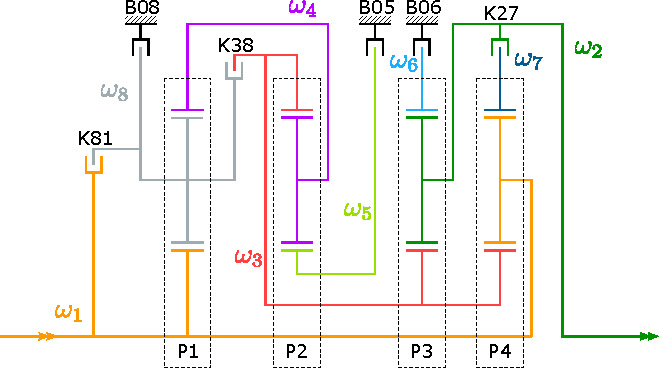
\includegraphics[scale=1]{figures/02_Modellierung/gearbox_schematic_color_with_labels.pdf}
	\caption{Schematischer Aufbau des Getriebes.}
	\label{fig:gearbox} % always use \label AFTER \caption
\end{figure}

\subsection{Anwendung des Newton-Euler-Formalismus}\label{ssec:AnwNE}
Die Wellen und Planeten rotieren alle nur um eine Achse bzw. bewegen sich nur auf einer Kreisbahn. Daher werden die Orientierungen und Ortsvektoren des einzelnen Körper als skalare angegeben. Die Ortsvektoren werden als Zylinderkoordinaten geschrieben. Somit ergibt sich der Vektor der Orientierungen der einzelnen Wellen und der Planeten zu 
\begin{equation}
\pmb{s} = \begin{bmatrix} s_{1}\quad s_{2}\quad \dots \quad s_{12} \end{bmatrix}^T = \begin{bmatrix} \phi_{1}\quad \phi_{2}\quad \dots \quad \phi_{12} \end{bmatrix}^T.
\end{equation} 
Die Ortsvektoren der Wellen 1-8 können aufgrund der nicht vorhanden translatorischen Bewegung gleich Null gesetzt werden. Lediglich die Planeten haben durch die Bewegung auf den Planetenträgern um die Drehachse einen translatorischen Anteil. Die Position der Planeten ergibt sich somit aus den entsprechenden Radien der Planetenträgern $r_{T,j}$ und der Orientierung der Planetenträgern. Damit kann der Orstvektor des Systems geschrieben werden als
\begin{equation}
\pmb{r} = \begin{bmatrix} r_{1}\; r_{2}\; \dots \; r_{12} \end{bmatrix}^T = \begin{bmatrix} 0\; \dots \; 0 \quad r_{T,1}\,\phi_8 \quad r_{T,2}\,\phi_4 \quad r_{T,3}\,\phi_2 \quad r_{T,4}\,\phi_1 \end{bmatrix}^T
\end{equation}
Da das MKS $f=4$ FHG hat lässt sich nach \cite{Schiehlen.2017} dieses durch verallgemeinerte Koordinaten $\pmb{y}\in \mathbb{R}^f$ beschreiben. Dabei liegt es nahe, die zu den am Getriebe gemessenen Winkelgeschwindigkeiten gehörigen Winkel $\phi_{1}$, $\phi_{2}$ und $\phi_{8}$ zu verwenden. Zudem wird $\phi_{3}$ als weiterer FHG gewählt. Dadurch ergibt sich der Vektor der verallgemeinerten Koordinaten zu
\begin{equation}
\pmb{y} = \begin{bmatrix} \phi_{1}\quad \phi_{2}\quad \phi_{3}\quad \phi_{8} \end{bmatrix}^T.
\end{equation}
Die Zusammenhänge in (\ref{eq:zwangsbedingungen}) gelten auch für die zugehörigen Winkel. Damit können $\pmb{s}$ und $\pmb{r}$ in Abhängigkeit der verallgemeinerten Koordinaten angegeben werden. Die Einträge von $\pmb{s}(\pmb{y})$ ergeben sich zu 
\begin{subequations}\label{eq:zwangsbedingungen_aufgelöst}
	\begin{align}
	 	\phi_1 &= \phi_1 \\
	 	\phi_2 &= \phi_2 \\
	 	\phi_3 &= \phi_3 \\ \label{eq:s4}
		\phi_{4} &= -\frac{z_{\mathrm{S,1}} }{z_{\mathrm{H,1}} } \phi_1 +\left(\frac{z_{\mathrm{S,1}} }{z_{\mathrm{H,1}} }+1\right) \phi_8 \\
		\phi_{5} &= \left(-\frac{z_\mathrm{S,1} }{z_\mathrm{H,1} }-\frac{z_\mathrm{H,2} z_\mathrm{S,1}}{z_\mathrm{H,1} z_\mathrm{S,2}} \right) \phi_1
			-\frac{z_\mathrm{H,2} }{z_\mathrm{S,2}} \phi_3
			+\left(\frac{z_{\mathrm{S,1}} }{z_{\mathrm{H,1}} }+\frac{z_{\mathrm{H,2}} }{z_{\mathrm{S,2}} }+\frac{z_{\mathrm{H,2}} z_{\mathrm{S,1}}}{z_{\mathrm{H,1}} z_{\mathrm{S,2}}} +1\right) \phi_8 \\
		\phi_{6} &= \left(\frac{z_{\mathrm{S,3}} }{z_{\mathrm{H,3}} }+1\right) \phi_2 - \frac{z_{\mathrm{S,3}} }{z_{\mathrm{H,3}} } \phi_3 \\
		\phi_{7} &= \left(\frac{z_{\mathrm{S,4}} }{z_{\mathrm{H,4}} }+1\right) \phi_1 - \frac{z_{\mathrm{S,4}} }{z_{\mathrm{H,4}} } \phi_3 \\
		\phi_8 &= \phi_8 \\
		\phi_{9} &= -\frac{z_{\mathrm{S,1}} }{z_\mathrm{P,1} } \phi_1 +\left(\frac{z_\mathrm{S,1} }{z_\mathrm{P,1}} +1\right) \phi_8 \\
		\phi_{10} &= \left(\frac{z_\mathrm{H,2} z_\mathrm{S,1}}{z_\mathrm{H,1} z_\mathrm{P,2}} + \frac{z_\mathrm{S,1}}{z_\mathrm{H,1}} \right) \omega_1
			+\frac{z_\mathrm{H,2}}{z_\mathrm{P,2}} \phi_3
			+\left(\frac{z_\mathrm{S,1}}{z_\mathrm{H,1}} -\frac{z_\mathrm{H,2} }{z_\mathrm{P,2} }-\frac{z_\mathrm{H,2}  z_\mathrm{S,1}}{z_\mathrm{H,1}  z_\mathrm{P,2}} + 1\right) \phi_8 \\
		\phi_{11} &= \left( \frac{z_{\mathrm{S,3}}}{z_{\mathrm{P,3}}} + 1 \right) \phi_2 -\frac{z_{\mathrm{S,3}}}{z_{\mathrm{P,3}}} \phi_3 \\
		\phi_{12} &= \left( \frac{z_{\mathrm{S,4}}}{z_{\mathrm{P,4}}} + 1 \right) \phi_1 -\frac{z_{\mathrm{S,4}}}{z_{\mathrm{P,4}}} \phi_3
	\end{align}
\end{subequations}
Die Einträge von $\pmb{r}$ sind bis auf den Zehnten bereits in Abhängigkeit von $\pmb{y}$ angegeben. Der verbleibende Eintrag kann mit (\ref{eq:s4}) wie folgt angegeben werden
\begin{equation}
r_{10}(\pmb{y}) = r_{T,2}\,\phi_4 = r_{T,2}\,\left(-\frac{z_{\mathrm{S,1}} }{z_{\mathrm{H,1}} } \phi_1 +\left(\frac{z_{\mathrm{S,1}} }{z_{\mathrm{H,1}} }+1\right) \phi_8\right).
\end{equation}
Durch die zeitliche Ableitung von $\pmb{r}(\pmb{y})$ und $\pmb{s}(\pmb{y})$ gemäß (\ref{vi}) und \ref{omegai} erhält man die Jacobi-Matrizen der Translation
\begin{equation}
\pmb{J}_\mathrm{T} = \begin{bmatrix}
J_\mathrm{T1} & J_\mathrm{T2} & \cdots & J_\mathrm{T12}
\end{bmatrix}^T
\end{equation}  
und der Rotation 
\begin{equation}
\pmb{J}_\mathrm{R} = \begin{bmatrix}
J_\mathrm{R1} & J_\mathrm{R2} & \cdots & J_\mathrm{R12}
\end{bmatrix}^T,
\end{equation} 
welche die einzelnen Jacobi-Matrizen der Körper enthalten. Die Terme $\overline{\pmb{v}}$ und $\overline{\pmb{\omega}}$ verschwinden, da es sich um skleronome Bindungen handelt und die ZB (\ref{eq:zwangsbedingungen}) nicht explizit zeitabhängig sind. Auch die lokalen Beschleunigungsvektoren $\overline{\pmb{a}}$ und $\overline{\pmb{\omega}}$ verschwinden, da $\pmb{J}_\mathrm{T}$ und $\pmb{J}_\mathrm{R}$ zeitlich konstant sind. In der allgemeinen Bewegungsgleichung für holonome MKS (\ref{Bwg}) verschwinden somit die Zentrifugalkräfte in $\pmb{k}(\pmb{y},\dot{\pmb{y}},t)$. Auch die Corioliskräfte verschwinden, da für alle Körper das Inertialsystem als Referenzsystem verwendet wird. Im Vektor der verallgemeinerten Kräfte $\pmb{q}(\pmb{y},\dot{\pmb{y}},t)$ werden die eingeprägten Kräfte $\pmb{f}^e_i$ vernachlässigt da die translatorischen Bewegungen im Getriebe sehr klein gegenüber der rotatorischen Bewegungen sind. Somit reduziert sich (\ref{Bwg}) auf
\begin{equation}
\pmb{M}(\pmb{y},t)\cdot\ddot{\pmb{y}} = \pmb{q}(\pmb{y},\dot{\pmb{y}},t)
\end{equation}
wobei die Massenmatrix mit $\pmb{J}_\mathrm{T}$ und $\pmb{J}_\mathrm{R}$ jetzt angegeben werden kann als 
  \begin{equation}
\pmb{M}(\pmb{y},t) = \pmb{J}_\mathrm{T}^T\cdot\mathrm{diag}(m_i)\cdot\pmb{J}_\mathrm{T}+\pmb{J}_\mathrm{R}^T\cdot\mathrm{diag}(I_i)\cdot\pmb{J}_\mathrm{R}
\end{equation}
und der Vektor der verallgemeinerten Kräfte als
  \begin{equation}
\pmb{q}(\pmb{y},\dot{\pmb{y}},t) = \pmb{J}_\mathrm{R}^T\cdot\mathrm{\pmb{l}}^e 
\end{equation}
Die eingeprägten Momente sind die von den Schaltelementen aufgebrachten Momente $\mathrm{T}_{\mathrm{B05}}$, $\mathrm{T}_{\mathrm{B06}}$, $\mathrm{T}_{\mathrm{B08}}$, $\mathrm{T}_{\mathrm{K81}}$, $\mathrm{T}_{\mathrm{K38}}$ und $\mathrm{T}_{\mathrm{K27}}$. Des Weitern wirken am Getriebeeingang das Moment $\mathrm{T}_{\mathrm{In}}$ und am Getriebeausgang das Moment $\mathrm{T}_{\mathrm{Out}}$. Damit ergibt sich der Vektor der eingeprägten Momente zu
\begin{equation}\label{eq:le}
\mathrm{\pmb{l}}^e = \begin{bmatrix} \mathrm{T}_{\mathrm{In}}+\mathrm{T}_{\mathrm{K81}} \\ -\mathrm{T}_{\mathrm{K27}}-\mathrm{T}_{\mathrm{Out}} \\ -\mathrm{T}_{\mathrm{K38}} \\ 0 \\ \mathrm{T}_{\mathrm{B05}} \\ \mathrm{T}_{\mathrm{B06}} \\ \mathrm{T}_{\mathrm{K27}} \\ \mathrm{T}_{\mathrm{B08}}+\mathrm{T}_{\mathrm{K38}}-\mathrm{T}_{\mathrm{K81}} \\ 0 \\ 0 \\ 0 \\ 0 \end{bmatrix}.
\end{equation}
Das Eingangsmoment $\mathrm{T}_{\mathrm{In}}$ wird vom Verbrennungsmotor und einem Elektromotor gestellt. Das Ausgangssmoment $\mathrm{T}_{\mathrm{Out}}$ wird an die Kardanwelle übertragen. Andere eingeprägte Momente, wie Schleppmomente oder Reibungen an den Lagern werden vernachlässigt. Mit Hilfe der ersten Summe von (\ref{Bwg_lang}) können die Einträge der 4x4-Massenmatrix $\pmb{M}$ berechnet werden. Diese ergeben sich zu
\begin{align*}
	\pmb{M}_{(1,1)} &=  J_1+J_7\left(\frac{z_\mathrm{S,4}}{z_\mathrm{H,4}}+1\right)^2+J_{12} \left(\frac{z_\mathrm{S,4}}{z_\mathrm{P,4}}+1\right)^2+J_{10} {\left(\frac{z_\mathrm{S,1}}{z_\mathrm{H,1}} - \sigma_{5}\right)}^2+J_{5} \left(\frac{z_\mathrm{S,1}}{z_\mathrm{H,1}}+\sigma_{4}\right)^2 \\
		&\qquad + m_\mathrm{P,4} {r_\mathrm{T,4}}^2+\frac{J_{4} {z_\mathrm{S,1}}^2}{{z_\mathrm{H,1}}^2}+\frac{J_{9} {z_\mathrm{S,1}}^2}{{z_\mathrm{P,1}}^2}+\frac{m_\mathrm{P,2} {r_\mathrm{T,2}}^2 {z_\mathrm{S,1}}^2}{{z_\mathrm{H,1}}^2}\\
	%
	\pmb{M}_{(1,3)} &= \frac{J_{5} z_\mathrm{H,2} \left(\frac{z_\mathrm{S,1}}{z_\mathrm{H,1}}+\sigma_{4}\right)}{z_\mathrm{S,2}}-\frac{J_{12} z_\mathrm{S,4} \left(\frac{z_\mathrm{S,4}}{z_\mathrm{P,4}}+1\right)}{z_\mathrm{P,4}}-\frac{J_{10} z_\mathrm{H,2} \left(\frac{z_\mathrm{S,1}}{z_\mathrm{H,1}} - \sigma_{5}\right)}{z_\mathrm{P,2}}-\frac{J_{7} z_\mathrm{S,4} \left(\frac{z_\mathrm{S,4}}{z_\mathrm{H,4}}+1\right)}{z_\mathrm{H,4}}\\
	%
	\pmb{M}_{(1,4)} &= J_{10} \left(\frac{z_\mathrm{S,1}}{z_\mathrm{H,1}}-\sigma_{5}\right) \sigma_{3} - J_{5} \left(\frac{z_\mathrm{S,1}}{z_\mathrm{H,1}}+\sigma_{4}\right) \sigma_{2} -\frac{J_{4} z_\mathrm{S,1} \left(\frac{z_\mathrm{S,1}}{z_\mathrm{H,1}}+1\right)}{z_\mathrm{H,1}}\\
		&\qquad-\frac{J_{9} z_\mathrm{S,1} \left(\frac{z_\mathrm{S,1}}{z_\mathrm{P,1}}+1\right)}{z_\mathrm{P,1}}-\frac{m_\mathrm{P,2} {r_\mathrm{T,2}}^2 z_\mathrm{S,1} \left(\frac{z_\mathrm{S,1}}{z_\mathrm{H,1}}+1\right)}{z_\mathrm{H,1}}\\
	%
	\pmb{M}_{(2,2)} &= J_2+J_6 \left(\frac{z_\mathrm{S,3}}{z_\mathrm{H,3}}+1\right)^2+J_{11} \left(\frac{z_\mathrm{S,3}}{z_\mathrm{P,3}}+1\right)^2+m_\mathrm{P,3} {r_\mathrm{T,3}}^2\\
	%
	\pmb{M}_{(2,3)} &= -\frac{J_{6} z_\mathrm{S,3} \left(\frac{z_\mathrm{S,3}}{z_\mathrm{H,3}}+1\right)}{z_\mathrm{H,3}}-\frac{J_{11} z_\mathrm{S,3} \left(\frac{z_\mathrm{S,3}}{z_\mathrm{P,3}}+1\right)}{z_\mathrm{P,3}}\\
	\pmb{M}_{(3,1)} &= \pmb{M}_{(1,3)}\\
	\pmb{M}_{(3,2)} &= \pmb{M}_{(2,3)}\\
	\pmb{M}_{(3,3)} &= J_{3}+\frac{J_{10} {z_\mathrm{H,2}}^2}{{z_\mathrm{P,2}}^2}+\frac{J_{5} {z_\mathrm{H,2}}^2}{{z_\mathrm{S,2}}^2}+\frac{J_{6} {z_\mathrm{S,3}}^2}{{z_\mathrm{H,3}}^2}+\frac{J_{7} {z_\mathrm{S,4}}^2}{{z_\mathrm{H,4}}^2}+\frac{J_{11} {z_\mathrm{S,3}}^2}{{z_\mathrm{P,3}}^2}+\frac{J_{12} {z_\mathrm{S,4}}^2}{{z_\mathrm{P,4}}^2} \\
	%
	\pmb{M}_{(3,4)} &= -\frac{J_{10} z_\mathrm{H,2} \sigma_{3}}{z_\mathrm{P,2}} - \frac{J_{5} z_\mathrm{H,2} \sigma_{2}}{z_\mathrm{S,2}}\\
	\pmb{M}_{(4,1)} &= \pmb{M}_{(1,4)}\\
	\pmb{M}_{(4,3)} &= \pmb{M}_{(3,4)}\\
	%
	\pmb{M}_{(4,4)} &= J_8+J_4 \left(\frac{z_\mathrm{S,1}}{z_\mathrm{H,1}}+1\right)^2+J_{9} \left(\frac{z_\mathrm{S,1}}{z_\mathrm{P,1}}+1\right)^2+m_\mathrm{P,1} {r_\mathrm{T,1}}^2+J_{10} \sigma_{3}^2+J_5 \sigma_{2}^2 \\
		&\qquad + m_\mathrm{P,2} {r_\mathrm{T,2}}^2 \left(\frac{z_\mathrm{S,1}}{z_\mathrm{H,1}}+1\right)^2\\
	%
	\sigma_1 &= \left(\frac{z_{\mathrm{S,4}}}{z_{\mathrm{H,4}}}+1\right) \\
	\sigma_{2} &= \left(\frac{z_\mathrm{S,1}}{z_\mathrm{H,1}}+\frac{z_\mathrm{H,2}}{z_\mathrm{S,2}}+\frac{z_\mathrm{H,2} z_\mathrm{S,1}}{z_\mathrm{H,1} z_\mathrm{S,2}}+1\right)\\
	\sigma_{3} &= \left(\frac{z_\mathrm{H,2}}{z_\mathrm{P,2}}-\frac{z_\mathrm{S,1}}{z_\mathrm{H,1}}+\frac{z_\mathrm{H,2} z_\mathrm{S,1}}{z_\mathrm{H,1} z_\mathrm{P,2}}-1\right) \\
	\sigma_{5} &= \frac{z_\mathrm{H,2} z_\mathrm{S,1}}{z_\mathrm{H,1} z_\mathrm{P,2}} \\
	\sigma_{4} &= \frac{z_\mathrm{H,2} z_\mathrm{S,1}}{z_\mathrm{H,1} z_\mathrm{S,2}}
\end{align*}
wobei $J_{1-12}$ die Massenträgheitsmomente der entsprechenden Wellen sind und $m_{\mathrm{P},1-4}$ die Gesamtasse der Planeten eines Planetensatzes. Durch einsetzten von $\pmb{M}$ und \eqref{eq:le} in \eqref{Bwg_lang} ergeben sich die vier Gleichungen der Getriebedynamik
\begin{subequations} \label{eq:bewegungs_gleichungen}
	\begin{align}
		\pmb{M}_{(1,1)} \dot{\omega}_1 + \pmb{M}_{(1,3)} \dot{\omega}_3 +\pmb{M}_{(1,4)} \dot{\omega}_8
		&= T_{\mathrm{K81}} +T_{\mathrm{in}} + \sigma_1 T_{\mathrm{K27}}-T_{\mathrm{B05}} {\left(\frac{z_{\mathrm{S,1}} }{z_{\mathrm{H,1}}}+\sigma_{4} \right)}\\
		%
		\pmb{M}_{(2,2)} \dot{\omega}_2 + \pmb{M}_{(2,3)} \dot{\omega}_3
		&= T_{\mathrm{B06}} {\left(\frac{z_{\mathrm{S,3}} }{z_{\mathrm{H,3}} }+1\right)}-T_{\mathrm{out}} -T_{\mathrm{K27}} \\
		%
		\pmb{M}_{(3,1)} \dot{\omega}_1 + \pmb{M}_{(3,2)} \dot{\omega}_2 + \pmb{M}_{(3,3)} \dot{\omega}_3 + \pmb{M}_{(3,4)} \dot{\omega}_8
		&= -T_{\mathrm{K38}} -\frac{ z_{\mathrm{H,2}} }{z_{\mathrm{S,2}} }T_{\mathrm{B05}}-\frac{z_{\mathrm{S,3}}}{z_{\mathrm{H,3}}}T_{\mathrm{B06}}-\frac{z_{\mathrm{S,4}} }{z_{\mathrm{H,4}}}T_{\mathrm{K27}}\\
		%
		\pmb{M}_{(4,1)} \dot{\omega}_1 + \pmb{M}_{(4,3)} \dot{\omega}_3 + \pmb{M}_{(4,4)} \dot{\omega}_8
		&= T_{\mathrm{B08}} +T_{\mathrm{K38}} -T_{\mathrm{K81}} +\sigma_{2} T_{\mathrm{B05}}.
	\end{align}
\end{subequations}
Mit Hilfe der Definition des Eingangsvektors
\begin{equation}\label{eq:u}
\pmb{u} = \begin{bmatrix} \mathrm{T}_{\mathrm{In}} \quad \mathrm{T}_{\mathrm{Out}} \quad \mathrm{T}_{\mathrm{K81}} \quad \mathrm{T}_{\mathrm{K38}} \quad \mathrm{T}_{\mathrm{B08}} \quad \mathrm{T}_{\mathrm{B05}} \quad \mathrm{T}_{\mathrm{B06}} \quad \mathrm{T}_{\mathrm{K27}} \end{bmatrix}^T
\end{equation}
lassen sich die Gleichungen \eqref{eq:bewegungs_gleichungen} zusammenfassen zu
\begin{equation}
\pmb{M}\,\ddot{\pmb{y}} = \tilde{\pmb{B}}\,\pmb{u}.
\end{equation}
Dieses Differentialgleichungssystem kann mit der Definition des Zustands
\begin{equation}
\pmb{x} = \dot{\pmb{y}} = \begin{bmatrix} \omega_1 \\ \omega_2 \\ \omega_3 \\ \omega_8\end{bmatrix}
\end{equation}
und der Invertierung von $\pmb{M}$ in die Zustandsraumdarstellung 
\begin{equation}
\dot{\pmb{x}} = \pmb{M}^{-1}\tilde{\pmb{B}}\,\pmb{u} = \pmb{B}\,\pmb{u}
\end{equation}
transformiert werden. In dieser Darstellung ist leicht ersichtlich, dass das System aufgrund der fehlenden Systemmatrix nicht zustandsabhängig ist.

\subsection{Erweiterung um elastische Seitenwellen}
Aufgrund der relativ elastischen Seitenwellen kann es im Antriebsstrang zu erheblichen Schwingungen kommen. Um diese bei der Simulation eines Schaltvorgang mit berücksichtigen zu können, soll das in \ref{ssec:AnwNE} hergeleitete Zustandsraummodell um die Elastizitäten erweitert werden. Die Seitenwellen werden dabei als Feder-Dämpfer-Systeme modelliert. Die Kardanwelle wird hingegen als starrer Körper betrachtet. Ein schematischen Aufbau des Antriebsstrangs zeigt Abbildung ???. Zunächst wird der Zustandsvektor um die Verdrehung der Seitenwellen~$\psi$ und die Raddrehzahl~$\omega_\mathrm{C}$ ergänzt, sodass sich der erweiterte Zustandsvektor
\begin{equation}
\pmb{x}_\mathrm{ex} = \begin{bmatrix} \omega_1 \\ \omega_2 \\ \omega_3 \\ \omega_8 \\ \phi \\ \omega_\mathrm{C} \end{bmatrix}
\end{equation}
ergibt. Wie in Abbildung \ref{fig:final_drive} veranschaulicht, ergibt sich die Verdrehung $\phi$ aus der Differenz der Verdrehung am linken Schnittufer der Seitenwellen $\phi_\mathrm{ss,p}$ und der des Rades $\phi_\mathrm{C}$, am rechten Schnittufer. Unter Berücksichtigung der starren Kardanwelle berechnet sich somit für die Verdrehung der Seitenwellen zu
\begin{equation}
\phi = \frac{\phi_2}{i_{\mathrm{D}}} - \phi_\mathrm{C},
\end{equation}  
wobei $i_{\mathrm{D}}$ die Übersetzungen des Differentials angibt. Entsprechend gilt der Zusammenhang auch für die Winkelgeschwindigkeiten
\begin{equation}\label{eq:dynphi}
\dot{\phi} = \frac{\omega_2}{i_{\mathrm{D}}} - \omega_\mathrm{C}.
\end{equation}
Des Weiteren kann am Rad das Momentengleichgewicht
\begin{equation}\label{eq:MggRad}
I^\mathrm{eff}_\mathrm{C}\,\dot{\omega}_\mathrm{C} = 2\,T_\mathrm{ss} - T_\mathrm{res},
\end{equation}
aufgestellt werden. Das effektive Massenträgheitsmomentes des Rads $I^\mathrm{eff}_\mathrm{C}$ setzt sich wie folgt zusammen
\begin{equation}
I^\mathrm{eff}_\mathrm{C} = I_\mathrm{ss} + m_\mathrm{C}\,r_\mathrm{dyn}.
\end{equation}
Dabei ist $I_\mathrm{ss}$ das Massenträgheitsmoment einer Seitenwelle, $m_\mathrm{C}$ die Masse des Rads und $r_\mathrm{dyn}$ der dynamische Radradius. Das Moment $T_\mathrm{ss}$ ist das von den Seitenwellen übertragene Moment und kann mit dem Steifigkeitskoeffizient $k_\mathrm{ss}$ und dem Dämpfungskoeffizient $d_\mathrm{ss}$ berechnet werden zu
\begin{equation}\label{eq:Tss}
T_\mathrm{ss} = k_\mathrm{ss}\left(\frac{\phi_2}{i_{\mathrm{D}}} - \phi_\mathrm{C}\right) + d_\mathrm{ss}\left(\frac{\omega_2}{i_{\mathrm{D}}} - \omega_\mathrm{C}\right) = k_\mathrm{ss} \phi + d_\mathrm{ss} \dot{\phi}.
\end{equation}
Das Fahrwiderstandsmoment $T_\mathrm{res}$ berechnet sich als Summe der berücksichtigten äußeren Fahrwiderstände zu
\begin{equation}\label{eq:Tres}
T_\mathrm{res} = r_\mathrm{dyn}\left(F_\mathrm{r}(v) + F_\mathrm{ad}(v) + F_\mathrm{g}\right). 
\end{equation}
Die berücksichtigten Widerstände sind der Rollwiderstand $F_\mathrm{r}(v)$, der Luftwiderstand $F_\mathrm{ad}(v)$ und die Hangabtriebskraft $F_\mathrm{g}$ und werden wie folgt berechnet
\begin{subequations}\label{eq:Fr_Fas_Fg}
\begin{align}
F_\mathrm{r}(v) &= v \cdot f_\mathrm{Roll}(v)\cdot \cos\left(\zeta\right)\cdot m_\mathrm{veh}\cdot g, \\
F_\mathrm{ad}(v) &= \frac{1}{2}\cdot v^2\cdot\rho_\mathrm{Air}\cdot c_\mathrm{W}\cdot A_\mathrm{front},\\
F_\mathrm{g} &= \sin\left(\zeta \right)\cdot m_\mathrm{veh}\cdot g.
\end{align}
\end{subequations}
Dabei ist $v = \omega_\mathrm{C}\,r_\mathrm{dyn}$ die Fahrzeuggeschwindigkeit, $f_\mathrm{Roll}(v)$ der von der Geschwindigkeit abhängige Faktor
des Rollwiderstands, $\zeta$ die Steigung der Straße in rad, $g$ die Erdbeschleunigung, $\rho_\mathrm{Air}$ die Luftdichte, $c_\mathrm{W}$ der Widerstandsbeiwert des Fahrzeugs, $A_\mathrm{front}$ die Frontfläche des
Fahrzeugs und $m_\mathrm{veh}$ die Gesamtmasse des Fahrzeugs \cite[S.~3ff]{Naunheimer.2007}.
Das Einsetzten von \eqref{eq:Tss} und \eqref{eq:Tres} in \eqref{eq:MggRad} und anschließender Auflösung nach $\dot{\omega}_\mathrm{C}$ führt auf die Dynamik des Rades
\begin{equation}\label{eq:dynwc}
\dot{\omega}_\mathrm{C} = \left[ 2\,\left(k_\mathrm{ss}\left(\frac{\phi_2}{i_{\mathrm{D}}} - \phi_\mathrm{C}\right) + d_\mathrm{ss}\left(\frac{\omega_2}{i_{\mathrm{D}}} - \omega_\mathrm{C}\right)\right) - r_\mathrm{dyn}\left(F_\mathrm{r}(v) + F_\mathrm{ad}(v) + F_\mathrm{g}\right)\right]/I^\mathrm{eff}_\mathrm{C}.
\end{equation}
Aufgrund der angenommenen starren Verbindung von Welle 2, der Kardanwelle und des Differentials, werden die Massenträgheitsmomente dieser Bauteile zusammengefasst zu
\begin{equation}
J^\mathrm{eff}_2 = J_2 + J^\mathrm{eff}_\mathrm{cs} + \frac{J^\mathrm{eff}_\mathrm{ss}}{i_\mathrm{D}^2},
\end{equation}
wobei in das effektive Massenträgheitsmoment der Kardanwelle $J^\mathrm{eff}_\mathrm{cs} = J_\mathrm{cs} + 0,5\,J_\mathrm{D}$ die eine Hälfte des Massenträgheitsmoments des Differentials miteinbezogen wird. Die andere Hälfte wird aufgrund der Drehzahldifferenz nach dem Differential mit dem Massenträgheitsmoment der zweiten Seitenwelle $J^\mathrm{eff}_\mathrm{ss} =  0,5\,J_\mathrm{D} + J_\mathrm{ss}$ zusammen gefasst. Für das erweiterte System wird $J_2$ in $\pmb{M}(2,2)$ dann durch $J^\mathrm{eff}_2$ ersetzt. Des Weiteren wird in Abbildung \ref{fig:final_drive} ersichtlich, dass für das Ausgangsmoment 
\begin{equation}\label{eq:Tout}
T_\mathrm{out} = \frac{2\,T_\mathrm{ss}}{i_\mathrm{D}} = \frac{2}{i_\mathrm{D}}\,\left[ k_\mathrm{ss}\left(\frac{\phi_2}{i_{\mathrm{D}}} - \phi_\mathrm{C}\right) + d_\mathrm{ss}\left(\frac{\omega_2}{i_{\mathrm{D}}} - \omega_\mathrm{C}\right)\right]
\end{equation}
gilt und dieses in \eqref{eq:le} dementsprechend ersetzt werden kann.

Zu beachten ist hier, dass $v(\omega_\mathrm{C})$ zustandsabhängig ist und sowohl in $F_\mathrm{r}(v)$ als auch in $F_\mathrm{ad}(v)$ nichtlinear eingeht, wodurch das Gesamtsystem nichtlinear wird. Auch die Störgröße $\zeta(t)$ geht nichtlinear in die Widerstände ein. Damit lässt sich das erweiterte Modell mit 
den Gleichungen \eqref{eq:dynphi} und \eqref{eq:dynwc} in der Form 
\begin{equation}\label{eq:sys_nl}
\dot{\pmb{x}}_\mathrm{ex} = \pmb{f}(\pmb{x}_\mathrm{ex}) + \pmb{B}_\mathrm{ex,nl}\,\pmb{u}_\mathrm{ex,nl}
\end{equation}
schreiben.


Da in den weiteren Betrachtungen die Dynamik des Getriebes während eines Gangwechsels analysiert wird, kann das Modell auf zwei Gänge reduziert werden. In dieser Arbeit sind dies die Gänge Zwei und Drei. Wie Tabelle \ref{tbl:clutches} entnommen werden kann, sind die Schaltelemete B08 und K27 während beiden Gängen geöffnet daher gilt  
\begin{subequations}
\begin{align*}
T_\mathrm{K27} &= 0 \\
T_\mathrm{B08} &= 0.
\end{align*}
\end{subequations}
Des Weiteren sind in beiden Gängen die Schaltelemente K81 und B06 geschlossen. Daher gelten für beide Gänge die zusätzlichen Zwangsbedingungen
\begin{subequations}
\begin{align}
\omega_6 &= 0\\
\omega_1 &= \omega_8.
\end{align}
\end{subequations}
Damit ergeben sich der reduzierte Zustand und der reduzierte Eingang zu
\begin{equation}
\pmb{x}_\mathrm{ex,nl,23} = \begin{bmatrix} \omega_1 & \omega_2 & \phi & \omega_\mathrm{C}\end{bmatrix}^T
\end{equation}
und
\begin{equation}\label{eq:u_exnl23}
\pmb{u}_\mathrm{ex,nl,23} = \begin{bmatrix} \mathrm{T}_{\mathrm{In}} & \mathrm{T}_{\mathrm{K38}} & \mathrm{T}_{\mathrm{B05}} \end{bmatrix}^T.
\end{equation}
Durch Einsetzten der Zwangsbedingungen in \eqref{eq:zwangsbedingungen_aufgelöst} und der Berücksichtigung des reduzierten Zustands- und  Eingangsvektors ist das nichtlineare reduzierte System
\begin{equation}\label{eq:sys_nl23}
\dot{\pmb{x}}_\mathrm{ex,23} = \pmb{f}_{23}(\pmb{x}_\mathrm{ex,23}) + \pmb{B}_\mathrm{ex,nl23}\,\pmb{u}_\mathrm{ex,nl23}.
\end{equation}

\begin{figure}
   \centering
   \def\svgwidth{\columnwidth}
   \import{figures/02_Modellierung/}{final_drive_with_forces.pdf_tex}
   \caption{Schematische Darstellung des Abtriebsstrangs}
   \label{fig:final_drive}
\end{figure}


\section{Modellierung der Reibung an Kupplungen und Bremsen} \label{sec:mod_reib}
Die im Abschnitt \ref{ssec:AnwNE} eingeführten Momente der Schaltelemente werden über Lamellenkupplungen beziehungsweise -bremsen an den Wellen angebracht. Dabei werden die Lamellenpakete über einen hydraulischen Druck zusammengepresst, sodass zwischen den Flächen Reibkräfte wirken. Solang die aus dem Druck resultierende Normalkraft an Lamellenpaketen nicht ausreicht um die Scheiben gegeneinander abzustützen, wirkt die Reibkraft entgegen der Differnzdrehzahl $\Delta \omega$ der drehenden Scheiben. Ist die Normalkraft groß genug entsteht eine kraftschlüssige Verbindung zwischen Innen- und Außenlamellen. In diesem Fall ist $\Delta \omega = 0$ und der Betrag der Reibkraft entspricht dem der Reaktionskraft und wirkt dieser entgegen.   

Zur Ermittlung der auf die Wellen wirkenden Reaktionsmomente bedarf es eines Reibmodells. Im Wesentlichen können diese in statische und dynamische Reibmodelle eingeteilt werden. Dynamische Reibmodelle unterscheiden sich dadurch, dass sie über mindestens einen weiteren Zustand verfügen. Dies ermöglicht die Simulation von weiteren Reibeffekten wie Hysteresen, variierende Losbrechkräfte oder nicht-gleitende Auslenkungen \cite{Schroeder.2015}. Im folgenden werden statische und dynamische Reibmodelle erläutert.

\subsection{Statische Reibmodelle}
Die einfachste Art der Reibungsmodellierung ist die Coulombsche Reibung. Dabei ist die Reibkraft proportional zur Normalkraft $F_\mathrm{N}$ und einem konstanten Reibungskoeffizienten $\mu_\mathrm{C}$. Nach \cite{Schroeder.2015} ist diese definiert als
\begin{equation}
F_\mathrm{C} = F_\mathrm{N}\,\mu_\mathrm{C}\;\mathrm{sign}(\Delta \omega)=F_\mathrm{N}\,\mu_\mathrm{C}\begin{cases}1&\quad,\Delta \omega>0\\0&\quad,\Delta \omega=0\\-1&\quad,\Delta \omega<0 \end{cases}
\end{equation}
Durch die Erweiterung um einen Haftreibungsbeiwert $\mu_\mathrm{S}$, wird eine benötigte Losbrechkraft mit berücksichtigt. Der Haftreibungsbeiwert $\mu_\mathrm{S}$ ist im Normalfall größer als $\mu_\mathrm{C}$, sodass eine größere Kraft notwendig ist um einen reibungsbehafteten Körper aus der ruhe zu bringen. Für die Haftreibung gilt
\begin{equation}
F_\mathrm{S} = \begin{cases}F_\mathrm{A}&,\vert F_\mathrm{A}\vert < F_\mathrm{N}\,\mu_\mathrm{S} (\wedge\Delta \omega = 0)
\\ F_\mathrm{N}\,\mu_\mathrm{S}\,\mathrm{sign}(F_\mathrm{A})&,\vert F_\mathrm{A}\vert \geq F_\mathrm{N}\,\mu_\mathrm{S} (\wedge\Delta \omega = 0) \end{cases}
\end{equation}
wobei $F_\mathrm{A}$ die Summe der äußeren Kräfte ist. Sind die Reibflächen geschmiert, ist eine Änderung der Reibkennlinie über  die $\Delta \omega$ zu beobachten. Dieses Phänomen berücksichtigt die viskose Reibung. Diese ist definiert als
\begin{equation}
F_\mathrm{V}=\nu\vert\Delta\omega\vert^{\delta_\mathrm{V}}\mathrm{sign}(\Delta\omega)
\end{equation}
mit dem viskosen Reibungsexponenten $\delta_\mathrm{V}$ und dem Reibkoeffizienten $\nu$. Des weiteren lässt sich $F_\mathrm{C}$ durch die Stribeck-Funktion erweitern. Damit wird das rapide Abfallen der Reibkraft bei kleinen Geschwindigkeiten berücksichtigt. Dieser Effekt entsteht durch das Aufbrechen von Kontaktstellen und der anschließenden Bildung eines Schmierfilms \cite{Stribeck.1903}. Eine übliche Modellierung der Stribeck-Funktion ist
\begin{equation}
F_\mathrm{Stribeck} = F_\mathrm{C} + F_\mathrm{N}(\mu_\mathrm{S}-\mu_\mathrm{C})\mathrm{exp}\left[-\left(\frac{\vert\Delta \omega \vert}{\omega_\mathrm{S}}\right)^{\delta_\mathrm{S}}\right]
\end{equation} 
mit der Stribeck-Geschwindigkeit $\omega_\mathrm{S}$ und dem Stribeck-Exponent $\delta_\mathrm{S}$. Die verschiedene statischen Reibmodelle lassen sich zum "Kinetischen Reibmodell" 
\begin{equation}
F_\mathrm{Kin} = \begin{cases}F_\mathrm{A} &,\Delta \omega=0 \\
 F_\mathrm{Stribeck}\; \mathrm{sign}(\Delta \omega)+F_\mathrm{V} &, \Delta \omega \neq 0\end{cases}
\end{equation}
zusammenfassen \cite{Altpeter.1999}.

Eine Schwäche dieses Modells ist der unstetige Verlauf der Reibkennlinie bei $\Delta \omega=0$. Diese Schwäche kann durch die Annäherung der Reibkennlinie über eine stetige atan-Funktion behoben werden. Dennoch bedarf es weiterhin der Unterscheidung zwischen Haft- und Gleitbereich. Hierfür ist entweder eine variable Zeitschrittweite des Solvers notwendig oder die Definition eines Geschwindigkeitbandes um $\Delta\omega=0$. Des weiteren ist die Reibkraft im Haftbereich von den äußeren Kräften abhängig, welche hier nicht bekannt sind und durch das Modell berechnet werden sollen. Aus diesen Gründen werden im Folgenden dynamische Reibmodelle betrachtet, welche diese Schwächen nicht aufweisen. 

\subsection{Dynamische Reibmodelle}
Um die dynamischen Reibeffekte vorallem um $\Delta\omega=0$ mit berücksichtigen zu können werden dynamische Reibmodelle benötigt. Einen ersten Ansatz dazu liefert das Reibmodell von Dahl. Dieses beschreibt die dynamischen Reibeffekte für kleine Auslenkungen mit kleinen Federn in den Kontaktbereichen von Körpern und geht anschließend in die Coulombschen-Reibung über \cite{Schroeder.2015}. Die Reibdynamik des Dahlschen-Modells wird definiert durch die Differentialgleichung
\begin{equation}
F_\mathrm{R,Dahl} = \left[\sigma_0\ \vert 1-\frac{F_\mathrm{R,Dahl}}{F_\mathrm{C}}\mathrm{sign}(\Delta\omega)\vert^\beta\ \mathrm{sign}\left( 1-\frac{F_\mathrm{R,Dahl}}{F_\mathrm{C}}\mathrm{sign}(\Delta\omega)\right)\right]\Delta\omega
\end{equation}
mit der zuvor definierten Coulomschen-Reibkraft $F_\mathrm{C}$, der Federsteifigkeit $\sigma_0$ und dem Formparameter der Hysterese $\beta$. Das Lund-Grenoble (LuGre) Reibmodell erweitert das Modell von Dahl um einen Dämpfungsanteil und ersetzt die Coulombsche-Kraft durch einen beliebige Reibkraftkennlinie $F_\mathrm{SS}$. Die Kontaktstellen der Reibflächen werden dabei als "Borsten"  modelliert, welche die Borstensteifigkeit $\sigma_0$ und die Borstendämpfung $\sigma_1$ besitzen. Mit der Borstenauslenkung $z$ lässt sich die LuGre-Reibkraft angeben als
\begin{equation}
F_\mathrm{R,LuGre} = \sigma_0\, z + \sigma_1 \dot{z} + \sigma_2\, \Delta \omega\quad \mathrm{mit}\  \dot{z}=\Delta\omega\left(1-\frac{\sigma_0 z}{F_\mathrm{SS}}\right)
\end{equation} 
wobei $\sigma_2$ der Steigungskoeffizienten der viskosen Reibung ist und $z_\mathrm{SS} = F_\mathrm{SS}/\sigma_0$ die maximale Borstenauslenkung[Quelle aus Mahl ???]. Jedoch wird in \cite{Dupont.2002} gezeigt, dass dieses Modell kein elasto-plastisches Presliding abbilden kann. Daher führt jede nichtkonstante Reibkraft zu einem sogenannten plastischen Presliding von $z$ wodurch es besonders bei periodischen Kräften zu einem physikalisch nicht existierenden Drift kommt. Das Elasto-Plastische Modell erweitert das LuGre-Modell um einen elastischen Bereich für kleine $z$. Nach \cite{Dupont.2000} ergibt sich die Dynamik der Auslenkung zu 
\begin{equation}
\dot{z} = \Delta \omega \left(1-\alpha(z,\Delta \omega)\frac{\sigma_0\,z}{F_\mathrm{SS}}\right)^i,\quad i\in \mathbb{Z}
\end{equation}
wobei $i=1$ gesetzt wird und die Funktion $\alpha(z)\in\left[0,1\right]$ ein elastische Bereich für kleine $z$ erzeugt. 

Aufgrund der erläuterten Vorteile wird das Elasto-Plastische-Modell für das Simulationsmodell verwendet. Dabei wird der viskose Reibungsanteil vernachlässigt ($\sigma_2 = 0$). Mit dem mittleren Radius $r_\mathrm{m}$ der Kupplungs- und Bremsscheiben und der Anzahl der Scheiben pro Schaltelement $N_\mathrm{disc}$  lassen sich die oben beschrieben Kräfte in Momente umrechnen. Letztendlich ergibt sich das an der Welle angreifende Reibmoment des Schaltelements $k$ zu
\begin{align}\label{eq:T_Cl}
T_{\mathrm{Cl},k} = \sigma_0\,z + \sigma_1\,\dot{z}
\end{align}
mit
\begin{align}
\dot{z} &= \Delta \omega \left(1-\alpha\frac{\sigma_0\,z}{T_\mathrm{Cl,ss}}\right)\\
T_\mathrm{Cl,SS} &= k_\mathrm{sign}(\Delta \omega,z)\,2\,N_{\mathrm{Disc},k}\,r_{\mathrm{m},k}\,\mu(p_\mathrm{N},T_\mathrm{Oil},\Delta \omega)F_\mathrm{N}.\label{eq:T_ClSS}
\end{align}
Der Reibwert $\mu(p_\mathrm{N},T_\mathrm{Oil},\Delta \omega)$ wird aus einem Kennfeld in Abhängigkeit der des Drucks an den Scheiben $p_\mathrm{N}$, der Öltemperatur $T_\mathrm{Oil}$ und $\Delta \omega$ gewonnen. Die Größe $k_\mathrm{sign}(\Delta \omega,z)$ definiert das Vorzeichen der Reibkraft. Zur Optimierung des numerischen Verhaltens des Simulationsmodells bei geschlossener Kupplung d.h. $\Delta \omega = 0$ wird dieser definiert zu 
\begin{equation}
k_\mathrm{sign}(\Delta \omega,z)=\begin{cases} \mathrm{sign}(z)\quad &,z\neq 0\\\mathrm{sign}(\Delta \omega)\quad &,z = 0\end{cases}.
\end{equation}
Die Normalkraft $F_\mathrm{N}$ ergibt sich aus $p_\mathrm{N}$ und der Fläche der Scheiben $A_\mathrm{Disc}$ und wird im Simulationsmodell vorgegeben. 

Mit $z_\mathrm{SS} = T_\mathrm{Cl,SS}/\sigma_0$ und $\lim_{z \rightarrow z_\mathrm{SS}}\alpha(z)=1$ konvergiert \eqref{eq:T_Cl} im Gleitbereich ($\Delta \omega \neq 0$) gegen $T_\mathrm{Cl,SS}$. 

\section{Beschreibung eines Gangwechsels}\label{sec:Gangwechsel}
Bei einem Gangwechsel wird durch die Betätigung von Schaltelementen die Übersetzung des Getriebes geändert. Dies soll zum einen in jedem Fall möglichst ohne für den Fahrer spürbare unerwünschte Beschleunigungen am Getriebeabtrieb passieren. Zum anderen soll der Gangwechsel aber auch so schnell wie möglich und ohne Momentenunterbrechung vollzogen werden. Es besteht also eine Zielkonflikt zwischen den Komfortansprüchen des Fahrers und der Dauer eines Schaltvorgangs. 

Grundsätzlich wird ein Gangwechsel auf zwei Ebenen unterschieden. Zum einen die Richtung der Übersetzung $i_\mathrm{Gang}$. Bei einer Hochschaltung wird $i_\mathrm{Gang}$ kleiner und entsprechend bei einer Rückschaltung größer. Zum anderen die Richtung des Antriebsmoments am Getriebeeingang. Ist dieses positiv spricht man von einer Zugschaltung bei negativem Antriebsmoment von einer Schubschaltung \cite{Fischer.2016}.
In dieser Arbeit werden die Betrachtungen auf eine Zug-Hoch-Schaltung zwischen dem zweitem und dem dritten Gang reduziert. Dies hat zum einen den Grund, dass in diesen Gängen der Drehmomentenwandler überbrückt und die Trennkupplung geschlossen ist, sodass deren Dynamik vernachlässigt werden kann. Zum anderen ist dies eine häufige Schaltung im Fahrzeugbetrieb. Die Erkenntnisse können jedoch auch auf andere Gangwechsel übertragen werden.

Bei dem in dieser Arbeit betrachteten Getriebe wird ein Gangwechsel mittels der Schließung und der simultanen Öffnung einer Bremse bzw. Kupplung realisiert. Bei der Schaltung zwischen dem zweiten und dritten Gang sind dies die Bremse $B_\mathrm{05}$ und die Kupplung $K_\mathrm{38}$. Der Gangwechsel wird in die vier Phasen 2. Gang, Momentenübergabe, Drehzahlsynchronisation und 3. Gang eingeteilt. Die Abbildungen \ref{fig:Gang23_Geschw}-\ref{fig:Gang23_Tandw} zeigen die vier Phasen des Gangwechsels der zur Auswertung der Sensitivitäten im Folgenden verwendet wird.

Im 2. Gang ist die Kupplung $K_\mathrm{38}$ geschlossen und überträgt das volle Antriebsmoment. Die Differenzdrehzahl $\Delta \omega_{38}$ der Wellen 3 und 8 ist somit gleich Null. Die Bremse $B_\mathrm{05}$ ist geöffnet und überträgt kein Drehmoment. Vor dem Gangwechsel wird die Kupplung $K_\mathrm{38}$ durch eine Reduzierung des anliegenden Drucks ins Schleifen gebracht, sodass sich an der Kupplung eine minimale Drehzahldifferenz ergibt. Dadurch wirkt an den Scheiben der Kupplung die Gleitreibung, welche somit der Reaktionskraft an den Kupplungen entspricht. Der Betrag der Geleitreibung kann, wie in \ref{sec:mod_reib} beschrieben, mit dem Reibungskoeffizient und der Normalkraft berechnet werden.

Somit kann während der Momentenübergabe das Drehmoment an $K_\mathrm{38}$ abgesenkt werden, während gleichzeitig $B_\mathrm{05}$ mit Hilfe einer Vorsteuerung derart geschlossenen wird, dass stets das volle Antriebsmoment übertragen wird und $K_\mathrm{38}$ im Schleifen gehalten wird. Die Herleitung einer derartigen Vorsteuerung kann \cite{Weber.2018} entnommen werden.    
  
Wenn $K_\mathrm{38}$ vollständig geöffnet ist d.h. kein Drehmoment mehr übertragen wird beginnt die Drehzahlsynchronisation. Diese kann auf zwei Arten vollzogen werden. Zum einen kann das Drehmoment an $B_\mathrm{05}$ überhöht werden, wodurch die Differenzdrehzahl $\Delta \omega_{05}$ auf Null gebracht wird und die Antriebsdrehzahl abgesenkt wird. Eine weitere Möglichkeit, die sich besonders bei Hybridgetrieben anbietet, ist die Drehzahlsynchronisation mittels einer Absenkung des Antriebsmomentes herzustellen. Mit einer E-Maschine kann die Absetzung dabei schneller und genauer vollzogen werden, als mit einem Verbrennungsmotor. Bei dem in dieser Arbeit betrachteten Gangwechsel werden beide Möglichkeiten gleichzeitig genutzt.

Am Ende der Drehzahlsynchronisation ist $\Delta \omega_{05}=0$ und die Getriebeübersetzung $i_\textrm{Gang}$ in \ref{fig:Gang23_Geschw} liegt auf dem Niveau des dritten Gangs.

\begin{figure}[h]
\centering
\newlength\fheight 
\setlength\fheight{8cm}
\newlength\fwidth 
\setlength\fwidth{13cm}
% This file was created by matlab2tikz.
%
%The latest updates can be retrieved from
%  http://www.mathworks.com/matlabcentral/fileexchange/22022-matlab2tikz-matlab2tikz
%where you can also make suggestions and rate matlab2tikz.
%
\definecolor{mycolor1}{rgb}{0.00000,0.44700,0.74100}%
\definecolor{mycolor2}{rgb}{0.85000,0.32500,0.09800}%
%
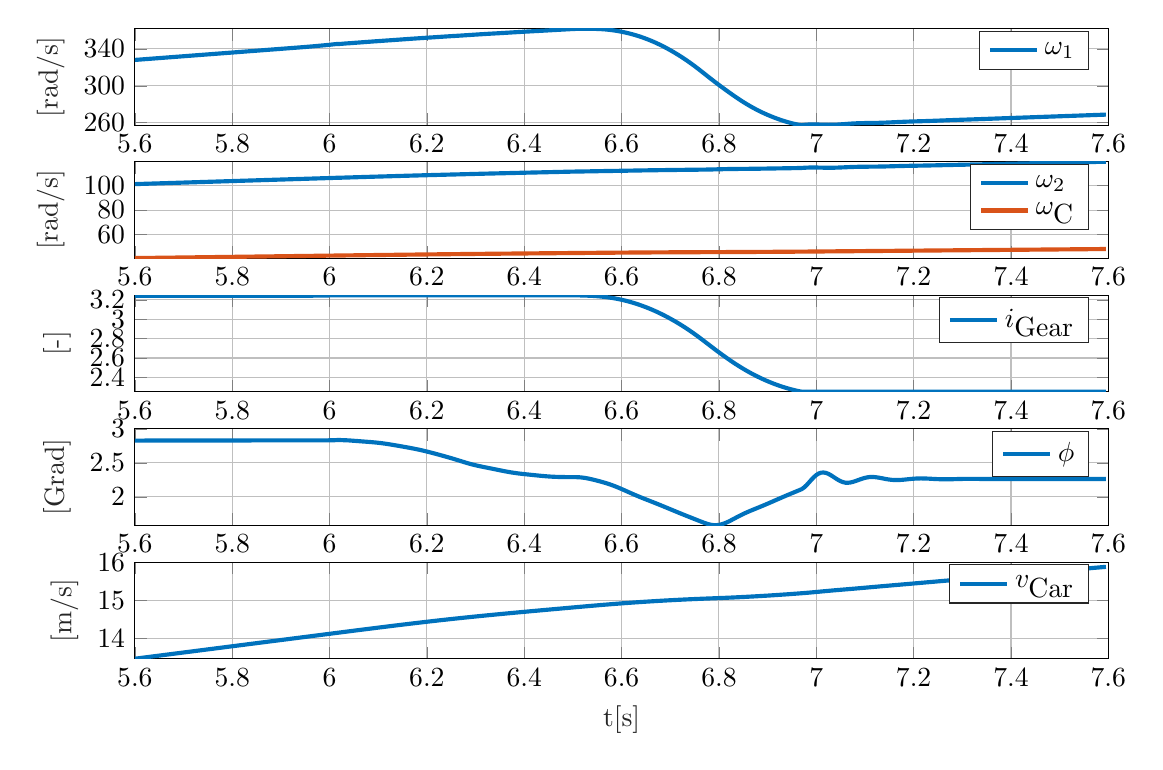
\begin{tikzpicture}

\begin{axis}[%
width=0.951\fwidth,
height=0.153\fheight,
at={(0\fwidth,0.847\fheight)},
scale only axis,
xmin=5.6,
xmax=7.6,
ymin=257.354045623529,
ymax=361.679637623739,
ytick={260,300,340,380},
ylabel style={font=\color{white!15!black}},
ylabel={[rad/s]},
axis background/.style={fill=white},
xmajorgrids,
ymajorgrids,
legend style={legend cell align=left, align=left, draw=white!15!black}
]
\addplot [color=mycolor1, line width=1.5pt]
  table[row sep=crcr]{%
5.6	327.973015972613\\
5.605	328.173196503571\\
5.61	328.373377189262\\
5.615	328.573558029248\\
5.62	328.77373902354\\
5.625	328.9739201717\\
5.63	329.17410147374\\
5.635	329.374282929225\\
5.64	329.574464538165\\
5.645	329.774646300127\\
5.65	329.974828215121\\
5.655	330.175010282715\\
5.66	330.37519250292\\
5.665	330.575374875305\\
5.67	330.775557399881\\
5.675	330.975740076218\\
5.68	331.175922904329\\
5.685	331.376105883782\\
5.69	331.576289014591\\
5.695	331.776472296327\\
5.7	331.976655729004\\
5.705	332.176839398926\\
5.71	332.377023359994\\
5.715	332.577207607051\\
5.72	332.777392092824\\
5.725	332.977576746185\\
5.73	333.177761520152\\
5.735	333.377946401713\\
5.74	333.578131405322\\
5.745	333.778316564264\\
5.75	333.978501911663\\
5.755	334.17868746763\\
5.76	334.378873242654\\
5.765	334.579059229031\\
5.77	334.779245419121\\
5.775	334.97943179968\\
5.78	335.179618366812\\
5.785	335.379805119474\\
5.79	335.579992066947\\
5.795	335.780179219412\\
5.8	335.980366594676\\
5.805	336.180554205209\\
5.81	336.380742070454\\
5.815	336.580930200169\\
5.82	336.781118613834\\
5.825	336.981307319995\\
5.83	337.181496341677\\
5.835	337.381685690897\\
5.84	337.581875399766\\
5.845	337.782065488441\\
5.85	337.982256003904\\
5.855	338.182446978476\\
5.86	338.382638480555\\
5.865	338.582830559391\\
5.87	338.783023314165\\
5.875	338.983216818814\\
5.88	339.183411218523\\
5.885	339.383606625394\\
5.89	339.583803255845\\
5.895	339.784001283118\\
5.9	339.984203437222\\
5.905	340.184423444781\\
5.91	340.384662688598\\
5.915	340.584920777348\\
5.92	340.785202123771\\
5.925	340.985519815592\\
5.93	341.186206389999\\
5.935	341.388354006297\\
5.94	341.592946524018\\
5.945	341.800935890059\\
5.95	342.013107812181\\
5.955	342.229420441504\\
5.96	342.449734053744\\
5.965	342.674934505967\\
5.97	342.905023399682\\
5.975	343.139630633068\\
5.98	343.378425455854\\
5.985	343.621540477615\\
5.99	343.867954470477\\
5.995	344.118352535604\\
6	344.372703897788\\
6.005	344.654072003652\\
6.01	344.966516209916\\
6.015	345.202428225592\\
6.02	345.262347786843\\
6.025	345.405345487616\\
6.03	345.663139985069\\
6.035	345.86931042348\\
6.04	346.023858169042\\
6.045	346.205383312853\\
6.05	346.420380257031\\
6.055	346.623722846069\\
6.06	346.813413472045\\
6.065	347.009737278534\\
6.07	347.213800688502\\
6.075	347.412748145835\\
6.08	347.605348430062\\
6.085	347.796908163182\\
6.09	347.988008802936\\
6.095	348.176093307189\\
6.1	348.360735466807\\
6.105	348.544353852605\\
6.11	348.728266935928\\
6.115	348.912424161481\\
6.12	349.096930333147\\
6.125	349.282631262076\\
6.13	349.469861139519\\
6.135	349.658283107268\\
6.14	349.847220090027\\
6.145	350.036168282051\\
6.15	350.224615339315\\
6.155	350.41184132042\\
6.16	350.597177640185\\
6.165	350.780237527707\\
6.17	350.960903795869\\
6.175	351.139232579521\\
6.18	351.315460282546\\
6.185	351.490023667203\\
6.19	351.663470234058\\
6.195	351.83631933629\\
6.2	352.009009191331\\
6.205	352.181857759664\\
6.21	352.355009170299\\
6.215	352.528398682487\\
6.22	352.701780572469\\
6.225	352.874775957789\\
6.23	353.046923886319\\
6.235	353.217736410717\\
6.24	353.386777509949\\
6.245	353.553718558233\\
6.25	353.718374705874\\
6.255	353.880429491596\\
6.26	354.041002086847\\
6.265	354.202305376821\\
6.27	354.366540001818\\
6.275	354.534641723053\\
6.28	354.705821095555\\
6.285	354.879307220587\\
6.29	355.054412681542\\
6.295	355.229925058381\\
6.3	355.403911945543\\
6.305	355.574658469269\\
6.31	355.741904114917\\
6.315	355.90488633502\\
6.32	356.063719047758\\
6.325	356.218735720006\\
6.33	356.370610140126\\
6.335	356.520388348996\\
6.34	356.669447911039\\
6.345	356.818940320103\\
6.35	356.969749937719\\
6.355	357.122493541639\\
6.36	357.277434235377\\
6.365	357.434356927307\\
6.37	357.592635532387\\
6.375	357.751435122682\\
6.38	357.909824855547\\
6.385	358.06685108315\\
6.39	358.221706286484\\
6.395	358.373874955784\\
6.4	358.523179234926\\
6.405	358.669778566807\\
6.41	358.814130628351\\
6.415	358.956942510867\\
6.42	359.099051843604\\
6.425	359.241298818347\\
6.43	359.384404482048\\
6.435	359.528896021368\\
6.44	359.675029853693\\
6.445	359.822774231398\\
6.45	359.971826637323\\
6.455	360.121680758037\\
6.46	360.271707493666\\
6.465	360.421251790185\\
6.47	360.569731678366\\
6.475	360.716723821903\\
6.48	360.862017644565\\
6.485	361.005639606492\\
6.49	361.14784167151\\
6.495	361.289059269372\\
6.5	361.429841566652\\
6.505	361.541963908227\\
6.51	361.609776061552\\
6.515	361.648421634541\\
6.52	361.669859428241\\
6.525	361.679637623739\\
6.53	361.679557373908\\
6.535	361.667668276279\\
6.54	361.63951111462\\
6.545	361.589004233596\\
6.55	361.51100234488\\
6.555	361.4002673758\\
6.56	361.251659202263\\
6.565	361.061522138762\\
6.57	360.827447907499\\
6.575	360.548123458717\\
6.58	360.22323881264\\
6.585	359.853096907383\\
6.59	359.438356285236\\
6.595	358.979737076568\\
6.6	358.477805196846\\
6.605	357.932795002571\\
6.61	357.344525811013\\
6.615	356.712407266668\\
6.62	356.035492617687\\
6.625	355.312594680318\\
6.63	354.542420530599\\
6.635	353.723715194602\\
6.64	352.855392726343\\
6.645	351.936635720995\\
6.65	350.966954412869\\
6.655	349.946200322662\\
6.66	348.874546816889\\
6.665	347.752423751474\\
6.67	346.580441473408\\
6.675	345.359291968297\\
6.68	344.089657474189\\
6.685	342.7721306054\\
6.69	341.4071534845\\
6.695	339.994983491629\\
6.7	338.535685530385\\
6.705	337.029147201719\\
6.71	335.475115179975\\
6.715	333.873245388733\\
6.72	332.223155302155\\
6.725	330.524474153146\\
6.73	328.77689168388\\
6.735	326.980187747693\\
6.74	325.134248819561\\
6.745	323.239066563037\\
6.75	321.294731529412\\
6.755	319.298439369855\\
6.76	317.262759463327\\
6.765	315.195513677176\\
6.77	313.111049203975\\
6.775	311.024463046329\\
6.78	308.947973351847\\
6.785	306.892958231272\\
6.79	304.864661964201\\
6.795	302.862130393347\\
6.8	300.883847836708\\
6.805	298.927676314899\\
6.81	296.992189418147\\
6.815	295.07672570102\\
6.82	293.182041972211\\
6.825	291.310387845389\\
6.83	289.465405433905\\
6.835	287.651724793431\\
6.84	285.874546537157\\
6.845	284.139068939194\\
6.85	282.450083471727\\
6.855	280.811524975373\\
6.86	279.226308696731\\
6.865	277.696148626036\\
6.87	276.221686650797\\
6.875	274.802555770197\\
6.88	273.437704078713\\
6.885	272.12557378135\\
6.89	270.864463934088\\
6.895	269.652682042429\\
6.9	268.488819107188\\
6.905	267.371785690578\\
6.91	266.300949687745\\
6.915	265.276046067966\\
6.92	264.297202295732\\
6.925	263.364768502307\\
6.93	262.479295064637\\
6.935	261.641348353161\\
6.94	260.851503415411\\
6.945	260.110194292244\\
6.95	259.417756304875\\
6.955	258.77432782773\\
6.96	258.179942889167\\
6.965	257.634472783561\\
6.97	257.354045623529\\
6.975	257.6646046711\\
6.98	257.903029942911\\
6.985	258.064783741053\\
6.99	258.141902522297\\
6.995	258.145997000496\\
7	258.103737849351\\
7.005	258.021335486802\\
7.01	257.925505249587\\
7.015	257.835165164343\\
7.02	257.766399541142\\
7.025	257.73087162692\\
7.03	257.738248881135\\
7.035	257.793174080001\\
7.04	257.894781899613\\
7.045	258.040477496337\\
7.05	258.21755673364\\
7.055	258.41433640153\\
7.06	258.620342801915\\
7.065	258.821672656543\\
7.07	259.011795814309\\
7.075	259.176839380176\\
7.08	259.31636097511\\
7.085	259.431120391346\\
7.09	259.519689621202\\
7.095	259.587291871016\\
7.1	259.639671663221\\
7.105	259.679762592514\\
7.11	259.713571589958\\
7.115	259.74814750626\\
7.12	259.791616257467\\
7.125	259.84664746329\\
7.13	259.914453615949\\
7.135	259.996656549938\\
7.14	260.091701537962\\
7.145	260.198941643773\\
7.15	260.315505245924\\
7.155	260.438631583401\\
7.16	260.564762565458\\
7.165	260.69002824374\\
7.17	260.812210189362\\
7.175	260.928923306729\\
7.18	261.038416097178\\
7.185	261.140171785139\\
7.19	261.234353827565\\
7.195	261.32168017479\\
7.2	261.403895198407\\
7.205	261.482869309665\\
7.21	261.560083457766\\
7.215	261.637101122048\\
7.22	261.715859598331\\
7.225	261.797604011416\\
7.23	261.883237558214\\
7.235	261.973155149336\\
7.24	262.067038856012\\
7.245	262.164687254383\\
7.25	262.265118623285\\
7.255	262.36726509506\\
7.26	262.470245621921\\
7.265	262.573187511688\\
7.27	262.675383659262\\
7.275	262.776133623499\\
7.28	262.874967284262\\
7.285	262.971583336586\\
7.29	263.066080777457\\
7.295	263.15879538407\\
7.3	263.249938851468\\
7.305	263.339978157013\\
7.31	263.42944027341\\
7.315	263.518876463882\\
7.32	263.60864789009\\
7.325	263.699278212111\\
7.33	263.790892127959\\
7.335	263.883521679553\\
7.34	263.977241506976\\
7.345	264.07189149822\\
7.35	264.167375686094\\
7.355	264.263463078194\\
7.36	264.359894256678\\
7.365	264.456397986991\\
7.37	264.552755758444\\
7.375	264.648736536723\\
7.38	264.744199017935\\
7.385	264.839102168345\\
7.39	264.933369224665\\
7.395	265.027121862653\\
7.4	265.120463901962\\
7.405	265.21348092786\\
7.41	265.306313184156\\
7.415	265.399081626459\\
7.42	265.491923552198\\
7.425	265.584939621357\\
7.43	265.67820278439\\
7.435	265.771753283947\\
7.44	265.865599802397\\
7.445	265.959721790524\\
7.45	266.054075696227\\
7.455	266.148601119166\\
7.46	266.243229135219\\
7.465	266.337889275918\\
7.47	266.432515821557\\
7.475	266.527055322531\\
7.48	266.621468228581\\
7.485	266.715731309006\\
7.49	266.80983769707\\
7.495	266.903795887061\\
7.5	266.997626644955\\
7.505	267.091359964407\\
7.51	267.185030795659\\
7.515	267.278675455565\\
7.52	267.37232826575\\
7.525	267.466017705013\\
7.53	267.559765227779\\
7.535	267.653584081963\\
7.54	267.747478983114\\
7.545	267.841446671469\\
7.55	267.935477348545\\
7.555	268.029556188752\\
7.56	268.123665514973\\
7.565	268.217786660489\\
7.57	268.311901749767\\
7.575	268.405995637223\\
7.58	268.500056427535\\
7.585	268.594077211152\\
7.59	268.688054694745\\
7.595	268.781989973118\\
};
\addlegendentry{$\omega_1$}

\end{axis}

\begin{axis}[%
width=0.951\fwidth,
height=0.153\fheight,
at={(0\fwidth,0.636\fheight)},
scale only axis,
xmin=5.6,
xmax=7.6,
ymin=40.9411242903612,
ymax=119.339202965924,
ylabel style={font=\color{white!15!black}},
ylabel={[rad/s]},
axis background/.style={fill=white},
xmajorgrids,
ymajorgrids,
legend style={legend cell align=left, align=left, draw=white!15!black}
]
\addplot [color=mycolor1, line width=1.5pt]
  table[row sep=crcr]{%
5.6	101.125007147652\\
5.605	101.186729473195\\
5.61	101.248451846443\\
5.615	101.31017426726\\
5.62	101.37189673565\\
5.625	101.433619251479\\
5.63	101.495341814749\\
5.635	101.557064425326\\
5.64	101.618787083214\\
5.645	101.680509788279\\
5.65	101.742232540525\\
5.655	101.803955339817\\
5.66	101.86567818616\\
5.665	101.927401079421\\
5.67	101.989124019602\\
5.675	102.050847006571\\
5.68	102.112570040333\\
5.685	102.174293120754\\
5.69	102.236016247838\\
5.695	102.297739421453\\
5.7	102.359462641603\\
5.705	102.421185908074\\
5.71	102.482909220071\\
5.715	102.544632578056\\
5.72	102.606355982476\\
5.725	102.668079433622\\
5.73	102.729802931708\\
5.735	102.791526476543\\
5.74	102.853250067852\\
5.745	102.914973705119\\
5.75	102.97669738799\\
5.755	103.03842111609\\
5.76	103.100144889331\\
5.765	103.161868707638\\
5.77	103.223592571168\\
5.775	103.285316479997\\
5.78	103.347040434327\\
5.785	103.408764434193\\
5.79	103.470488479705\\
5.795	103.532212570776\\
5.8	103.593936707401\\
5.805	103.655660889398\\
5.81	103.717385116688\\
5.815	103.779109389052\\
5.82	103.840833706395\\
5.825	103.902558068505\\
5.83	103.964282475313\\
5.835	104.026006926642\\
5.84	104.087731422463\\
5.845	104.149455962642\\
5.85	104.211180547183\\
5.855	104.272905175977\\
5.86	104.334629849031\\
5.865	104.396354566232\\
5.87	104.458079327552\\
5.875	104.519804132832\\
5.88	104.581528981973\\
5.885	104.643253874739\\
5.89	104.704978810926\\
5.895	104.766703790199\\
5.9	104.828428789337\\
5.905	104.890153768952\\
5.91	104.95187873951\\
5.915	105.013603726045\\
5.92	105.075328734922\\
5.925	105.137053737031\\
5.93	105.198776796748\\
5.935	105.260494084285\\
5.94	105.322202949905\\
5.945	105.38390226131\\
5.95	105.44559332003\\
5.955	105.507282739061\\
5.96	105.568975336429\\
5.965	105.630673398631\\
5.97	105.692380724001\\
5.975	105.754101294427\\
5.98	105.815836390854\\
5.985	105.877585390569\\
5.99	105.939344141712\\
5.995	106.001104189957\\
6	106.062860845193\\
6.005	106.129724102794\\
6.01	106.202810983133\\
6.015	106.26554771556\\
6.02	106.304124860576\\
6.025	106.35523051389\\
6.03	106.422768108335\\
6.035	106.482963772158\\
6.04	106.536272943804\\
6.045	106.594060195641\\
6.05	106.656998434327\\
6.055	106.718547792258\\
6.06	106.778401050756\\
6.065	106.839320773136\\
6.07	106.901245990124\\
6.075	106.962177626277\\
6.08	107.021846026197\\
6.085	107.080944342386\\
6.09	107.139527533129\\
6.095	107.197258170539\\
6.1	107.254170534149\\
6.105	107.31072698077\\
6.11	107.367233040934\\
6.115	107.423804362989\\
6.12	107.480558325796\\
6.125	107.53767845392\\
6.13	107.595225256735\\
6.135	107.653125596235\\
6.14	107.711211970049\\
6.145	107.769316364396\\
6.15	107.827260194229\\
6.155	107.884825900539\\
6.16	107.941823104253\\
6.165	107.998129570897\\
6.17	108.053697064356\\
6.175	108.108541736444\\
6.18	108.162740510035\\
6.185	108.216424850021\\
6.19	108.269757872043\\
6.195	108.322899954839\\
6.2	108.375988624147\\
6.205	108.429122074188\\
6.21	108.482344928085\\
6.215	108.535639622339\\
6.22	108.588933148184\\
6.225	108.642110258357\\
6.23	108.69502976777\\
6.235	108.74754220948\\
6.24	108.799513515842\\
6.245	108.850841606493\\
6.25	108.901468159609\\
6.255	108.951375608022\\
6.26	109.001035747863\\
6.265	109.051007140532\\
6.27	109.101812941741\\
6.275	109.153705059323\\
6.28	109.206575669072\\
6.285	109.260214173136\\
6.29	109.314345058035\\
6.295	109.368578008481\\
6.3	109.422359958746\\
6.305	109.475168523129\\
6.31	109.52692868278\\
6.315	109.57739308811\\
6.32	109.626560194387\\
6.325	109.674538785646\\
6.33	109.721557141208\\
6.335	109.767932117531\\
6.34	109.814065393667\\
6.345	109.860310608902\\
6.35	109.906955643148\\
6.355	109.954194906623\\
6.36	110.002101832767\\
6.365	110.050614480975\\
6.37	110.09955153244\\
6.375	110.148659120263\\
6.38	110.197647434745\\
6.385	110.246223874464\\
6.39	110.294142529277\\
6.395	110.341242069495\\
6.4	110.387462315614\\
6.405	110.432849215471\\
6.41	110.477541974148\\
6.415	110.521755198931\\
6.42	110.565743529142\\
6.425	110.609765435687\\
6.43	110.654044191643\\
6.435	110.698743417552\\
6.44	110.743943978421\\
6.445	110.789639170895\\
6.45	110.835739077627\\
6.455	110.882090122234\\
6.46	110.92850011738\\
6.465	110.974768276795\\
6.47	111.020715345303\\
6.475	111.066209744819\\
6.48	111.111184650463\\
6.485	111.155645950741\\
6.49	111.199668919346\\
6.495	111.243385484008\\
6.5	111.286963148873\\
6.505	111.326476010501\\
6.51	111.3599364749\\
6.515	111.390154293476\\
6.52	111.419741233839\\
6.525	111.450311102238\\
6.53	111.482819532196\\
6.535	111.517448126501\\
6.54	111.553821817973\\
6.545	111.591274978874\\
6.55	111.629008619738\\
6.555	111.66634434016\\
6.56	111.702695430614\\
6.565	111.737726454786\\
6.57	111.77136417231\\
6.575	111.803764304814\\
6.58	111.835280627755\\
6.585	111.866367169053\\
6.59	111.897506753115\\
6.595	111.929134794622\\
6.6	111.961585527127\\
6.605	111.995044905989\\
6.61	112.029537502262\\
6.615	112.064935705314\\
6.62	112.100982428715\\
6.625	112.137332485927\\
6.63	112.173598099124\\
6.635	112.209396106882\\
6.64	112.244390766456\\
6.645	112.278325915668\\
6.65	112.311044339041\\
6.655	112.342492821579\\
6.66	112.372716829559\\
6.665	112.40184096554\\
6.67	112.430046083051\\
6.675	112.457539308418\\
6.68	112.484526275687\\
6.685	112.511186790495\\
6.69	112.537656214437\\
6.695	112.564014854442\\
6.7	112.59028534479\\
6.705	112.61643693141\\
6.71	112.6423961464\\
6.715	112.66806167188\\
6.72	112.693319901151\\
6.725	112.71805984268\\
6.73	112.742187753337\\
6.735	112.765636049422\\
6.74	112.788368367548\\
6.745	112.810379316502\\
6.75	112.831692773247\\
6.755	112.852423364193\\
6.76	112.873411817625\\
6.765	112.896199019225\\
6.77	112.922640853486\\
6.775	112.954375334299\\
6.78	112.992271088282\\
6.785	113.036795927066\\
6.79	113.086522659965\\
6.795	113.139059378772\\
6.8	113.192160745349\\
6.805	113.243695590131\\
6.81	113.291841553258\\
6.815	113.335258816879\\
6.82	113.373207856742\\
6.825	113.405570999167\\
6.83	113.432786581897\\
6.835	113.455735661682\\
6.84	113.475582577112\\
6.845	113.493614378466\\
6.85	113.51108386661\\
6.855	113.529084806782\\
6.86	113.548464650577\\
6.865	113.56977803994\\
6.87	113.59328597027\\
6.875	113.618982794927\\
6.88	113.646656018657\\
6.885	113.675951438021\\
6.89	113.706449751767\\
6.895	113.737729119123\\
6.9	113.769421665048\\
6.905	113.801247000694\\
6.91	113.833032493383\\
6.915	113.864712523507\\
6.92	113.896317391505\\
6.925	113.927949611462\\
6.93	113.959758215272\\
6.935	113.991909459852\\
6.94	114.024563860449\\
6.945	114.057855122089\\
6.95	114.091880039321\\
6.955	114.126691072802\\
6.96	114.162300090754\\
6.965	114.198682134972\\
6.97	114.266609097247\\
6.975	114.401900087165\\
6.98	114.507622908556\\
6.985	114.579462774693\\
6.99	114.613846427011\\
6.995	114.615897406591\\
7	114.597422027448\\
7.005	114.561160589861\\
7.01	114.518935121215\\
7.015	114.479101496988\\
7.02	114.448792203667\\
7.025	114.433172888353\\
7.03	114.4365256406\\
7.035	114.460911746963\\
7.04	114.505954627114\\
7.045	114.57051412835\\
7.05	114.648967566754\\
7.055	114.736156322101\\
7.06	114.827482859476\\
7.065	114.916746058485\\
7.07	115.000946450715\\
7.075	115.074141246801\\
7.08	115.136049335774\\
7.085	115.187003642974\\
7.09	115.226368949758\\
7.095	115.256453731438\\
7.1	115.279798546699\\
7.105	115.297699312311\\
7.11	115.3128128689\\
7.115	115.328253991684\\
7.12	115.34762648973\\
7.125	115.372105573629\\
7.13	115.402235295555\\
7.135	115.438734311803\\
7.14	115.480915961417\\
7.145	115.528495210596\\
7.15	115.5802029189\\
7.155	115.634818364004\\
7.16	115.690767821117\\
7.165	115.746337703065\\
7.17	115.800546519914\\
7.175	115.85233856845\\
7.18	115.900938094332\\
7.185	115.946115329721\\
7.19	115.987941577259\\
7.195	116.026733535567\\
7.2	116.063262328393\\
7.205	116.098355301459\\
7.21	116.132667512697\\
7.215	116.166890038329\\
7.22	116.201880464872\\
7.225	116.238190512207\\
7.23	116.276220274566\\
7.235	116.316145046464\\
7.24	116.357824805545\\
7.245	116.401170872887\\
7.25	116.445749208164\\
7.255	116.491087545986\\
7.26	116.536795988522\\
7.265	116.582488364397\\
7.27	116.627851686549\\
7.275	116.672576016059\\
7.28	116.716453104724\\
7.285	116.759349345762\\
7.29	116.801308236162\\
7.295	116.842478121671\\
7.3	116.882952452087\\
7.305	116.922937688485\\
7.31	116.962666886091\\
7.315	117.002384126038\\
7.32	117.042248323005\\
7.325	117.082493462558\\
7.33	117.123172294924\\
7.335	117.164300512469\\
7.34	117.205911430366\\
7.345	117.247933920366\\
7.35	117.290325672709\\
7.355	117.332984614103\\
7.36	117.375795975168\\
7.365	117.418639740572\\
7.37	117.461419154829\\
7.375	117.504032039408\\
7.38	117.546415789631\\
7.385	117.588552165856\\
7.39	117.630407123191\\
7.395	117.672034422968\\
7.4	117.713479957661\\
7.405	117.754781543203\\
7.41	117.796001220426\\
7.415	117.837192486132\\
7.42	117.878416030506\\
7.425	117.919716546843\\
7.43	117.961126271494\\
7.435	118.002663068984\\
7.44	118.044330828333\\
7.445	118.086120488222\\
7.45	118.128012808234\\
7.455	118.169981085287\\
7.46	118.211994835101\\
7.465	118.254022880697\\
7.47	118.296036116832\\
7.475	118.338010910015\\
7.48	118.379929741004\\
7.485	118.421782311651\\
7.49	118.463565563134\\
7.495	118.505283234351\\
7.5	118.546944496705\\
7.505	118.588562608483\\
7.51	118.630153025712\\
7.515	118.671731813984\\
7.52	118.713314139188\\
7.525	118.75491265078\\
7.53	118.796536831272\\
7.535	118.838192538558\\
7.54	118.879881884831\\
7.545	118.921603436346\\
7.55	118.96335286398\\
7.555	119.005123614811\\
7.56	119.046907871546\\
7.565	119.088697376176\\
7.57	119.130484212864\\
7.575	119.172261684971\\
7.58	119.214024524552\\
7.585	119.255769669299\\
7.59	119.297495656703\\
7.595	119.339202965924\\
};
\addlegendentry{$\omega_2$}

\addplot [color=mycolor2, line width=1.5pt]
  table[row sep=crcr]{%
5.6	40.9411242903612\\
5.605	40.9661130055681\\
5.61	40.9911017400735\\
5.615	41.0160904938306\\
5.62	41.0410792668329\\
5.625	41.0660680590339\\
5.63	41.0910568704269\\
5.635	41.1160457009657\\
5.64	41.1410345506436\\
5.645	41.1660234194145\\
5.65	41.1910123072718\\
5.655	41.2160012141695\\
5.66	41.2409901401011\\
5.665	41.2659790850206\\
5.67	41.2909680489216\\
5.675	41.3159570317583\\
5.68	41.3409460335243\\
5.685	41.3659350541739\\
5.69	41.3909240937008\\
5.695	41.4159131520595\\
5.7	41.4409022292435\\
5.705	41.4658913253713\\
5.71	41.4908804401125\\
5.715	41.5158695735735\\
5.72	41.5408587257498\\
5.725	41.5658478965957\\
5.73	41.5908370861058\\
5.735	41.6158262942373\\
5.74	41.6408155209869\\
5.745	41.6658047663126\\
5.75	41.6907940302103\\
5.755	41.7157833126364\\
5.76	41.7407726135845\\
5.765	41.7657619330088\\
5.77	41.7907512709015\\
5.775	41.8157406272159\\
5.78	41.840730001944\\
5.785	41.8657193950399\\
5.79	41.8907088064963\\
5.795	41.9156982362685\\
5.8	41.9406876843503\\
5.805	41.9656771506982\\
5.81	41.9906666353064\\
5.815	42.0156561381318\\
5.82	42.0406456591687\\
5.825	42.0656351983738\\
5.83	42.0906247557408\\
5.835	42.1156143312256\\
5.84	42.1406039248211\\
5.845	42.1655935364824\\
5.85	42.1905831662016\\
5.855	42.215572813933\\
5.86	42.2405624796678\\
5.865	42.2655521633599\\
5.87	42.2905418649998\\
5.875	42.3155315845406\\
5.88	42.3405213219719\\
5.885	42.3655110772456\\
5.89	42.3905008503493\\
5.895	42.4154906412326\\
5.9	42.4404804484467\\
5.905	42.4654702718395\\
5.91	42.4904601125349\\
5.915	42.5154499702278\\
5.92	42.5404398445983\\
5.925	42.5654297352734\\
5.93	42.59041964069\\
5.935	42.6154095491356\\
5.94	42.640399436242\\
5.945	42.6653892613233\\
5.95	42.6903789679894\\
5.955	42.7153684943565\\
5.96	42.7403577872581\\
5.965	42.765346804387\\
5.97	42.7903355188569\\
5.975	42.8153239259309\\
5.98	42.840312048524\\
5.985	42.8652999207335\\
5.99	42.8902876372471\\
5.995	42.9152752590089\\
6	42.9402628475297\\
6.005	42.9652542352751\\
6.01	42.9902689040836\\
6.015	43.0153250690856\\
6.02	43.0403820478348\\
6.025	43.0654002350553\\
6.03	43.0903922301533\\
6.035	43.1153709622979\\
6.04	43.1403189186165\\
6.045	43.1652223312713\\
6.05	43.1900859698959\\
6.055	43.2149147790135\\
6.06	43.2397051497686\\
6.065	43.2644550906679\\
6.07	43.2891665079372\\
6.075	43.3138406637853\\
6.08	43.3384754745209\\
6.085	43.3630678316204\\
6.09	43.3876145561358\\
6.095	43.412111443738\\
6.1	43.4365524762989\\
6.105	43.4609314890439\\
6.11	43.4852428664018\\
6.115	43.5094810351788\\
6.12	43.5336411012665\\
6.125	43.5577190639003\\
6.13	43.5817122533054\\
6.135	43.6056189454089\\
6.14	43.6294378866308\\
6.145	43.6531683840006\\
6.15	43.676809843469\\
6.155	43.7003613982746\\
6.16	43.7238216351673\\
6.165	43.7471883308505\\
6.17	43.7704584239108\\
6.175	43.7936280126664\\
6.18	43.816692534301\\
6.185	43.8396470099513\\
6.19	43.862486316969\\
6.195	43.8852055146739\\
6.2	43.9078000981977\\
6.205	43.9302661810867\\
6.21	43.952600578795\\
6.215	43.974800816927\\
6.22	43.9968649977123\\
6.225	44.0187916059883\\
6.23	44.0405792840095\\
6.235	44.0622265881143\\
6.24	44.0837317454525\\
6.245	44.1050924950499\\
6.25	44.1263059965551\\
6.255	44.1473541320612\\
6.26	44.1682413956052\\
6.265	44.188990988516\\
6.27	44.2095853467352\\
6.275	44.2300248505961\\
6.28	44.250314078508\\
6.285	44.2704597564578\\
6.29	44.2904697046318\\
6.295	44.3103520935165\\
6.3	44.3301093421615\\
6.305	44.3497489298223\\
6.31	44.3692960201456\\
6.315	44.3887415334117\\
6.32	44.4080873533404\\
6.325	44.4273341876994\\
6.33	44.4464814128407\\
6.335	44.4655278358783\\
6.34	44.4844721116632\\
6.345	44.503313554719\\
6.35	44.5220525646704\\
6.355	44.5406909241674\\
6.36	44.5592320672781\\
6.365	44.5776808355189\\
6.37	44.5960431949066\\
6.375	44.6143257335168\\
6.38	44.6325351727676\\
6.385	44.650677838504\\
6.39	44.6687591807301\\
6.395	44.6867834838203\\
6.4	44.7047537696405\\
6.405	44.7226718197495\\
6.41	44.740538453099\\
6.415	44.7583538607979\\
6.42	44.7761180505916\\
6.425	44.7938312785727\\
6.43	44.8114944694323\\
6.435	44.8291094460848\\
6.44	44.8466791061615\\
6.445	44.8642073614784\\
6.45	44.8816989945291\\
6.455	44.8991593567883\\
6.46	44.9165940210365\\
6.465	44.9340084126451\\
6.47	44.9514074788455\\
6.475	44.9687954380736\\
6.48	44.98617565278\\
6.485	45.0035506190236\\
6.49	45.0209220901195\\
6.495	45.0382912967647\\
6.5	45.0556592326757\\
6.505	45.0730237872153\\
6.51	45.0903700604269\\
6.515	45.1076749342648\\
6.52	45.1249163040754\\
6.525	45.1420746576751\\
6.53	45.1591333156477\\
6.535	45.1760803333087\\
6.54	45.1929074877429\\
6.545	45.209606723452\\
6.55	45.2261772135695\\
6.555	45.2426141035564\\
6.56	45.2589101678486\\
6.565	45.275057657124\\
6.57	45.2910470772889\\
6.575	45.3068675019391\\
6.58	45.3225070743761\\
6.585	45.3379539996635\\
6.59	45.3531973866107\\
6.595	45.3682280427852\\
6.6	45.3830389895028\\
6.605	45.3976259685769\\
6.61	45.4119874133372\\
6.615	45.4261242049074\\
6.62	45.4400392703979\\
6.625	45.4537369442244\\
6.63	45.46722230167\\
6.635	45.4805004879603\\
6.64	45.4935761134689\\
6.645	45.5064528047892\\
6.65	45.519132929978\\
6.655	45.5316175174647\\
6.66	45.5439063147434\\
6.665	45.555998035159\\
6.67	45.5678906499513\\
6.675	45.5795817738044\\
6.68	45.5910690225104\\
6.685	45.6023503270298\\
6.69	45.6134241742035\\
6.695	45.624289745094\\
6.7	45.6349469510514\\
6.705	45.6453963816173\\
6.71	45.6556391709919\\
6.715	45.6656768110274\\
6.72	45.6755109550731\\
6.725	45.6851432305566\\
6.73	45.6945750538637\\
6.735	45.7038075176153\\
6.74	45.7128413260738\\
6.745	45.7216767970093\\
6.75	45.7303138818124\\
6.755	45.7387369587049\\
6.76	45.746976865704\\
6.765	45.7550227321265\\
6.77	45.7628844420224\\
6.775	45.7705825241749\\
6.78	45.7781474199802\\
6.785	45.7856176179394\\
6.79	45.793058602672\\
6.795	45.800535191317\\
6.8	45.8081050697241\\
6.805	45.8158197396308\\
6.81	45.8237251377708\\
6.815	45.8318570495616\\
6.82	45.8402407673786\\
6.825	45.8488908482278\\
6.83	45.8578125190732\\
6.835	45.8670030259277\\
6.84	45.8764542076791\\
6.845	45.8861543812258\\
6.85	45.8960908906542\\
6.855	45.9062515330852\\
6.86	45.9166262523683\\
6.865	45.9272075907856\\
6.87	45.9379913019808\\
6.875	45.9489758701538\\
6.88	45.9601623288739\\
6.885	45.9715532552354\\
6.89	45.9831523078709\\
6.895	45.9949631797664\\
6.9	46.0069893040462\\
6.905	46.0192330958139\\
6.91	46.0316960413844\\
6.915	46.0443783180349\\
6.92	46.0572792377091\\
6.925	46.0703971375588\\
6.93	46.083730002421\\
6.935	46.0972754378438\\
6.94	46.1110312769479\\
6.945	46.1249954770933\\
6.95	46.1391665900231\\
6.955	46.1535435122805\\
6.96	46.1681257988004\\
6.965	46.1829132859708\\
6.97	46.1979119135764\\
6.975	46.2133046709661\\
6.98	46.2292295290931\\
6.985	46.2457367346182\\
6.99	46.2628693147068\\
6.995	46.2805301684145\\
7	46.2985213178138\\
7.005	46.3167932129136\\
7.01	46.335153149845\\
7.015	46.3534646402439\\
7.02	46.3716124058533\\
7.025	46.3895129099247\\
7.03	46.4070967355262\\
7.035	46.4243310860751\\
7.04	46.4412230279886\\
7.045	46.4577918581975\\
7.05	46.4741308174776\\
7.055	46.4903251246984\\
7.06	46.5064503265645\\
7.065	46.5226089496622\\
7.07	46.5388515958738\\
7.075	46.5552742763651\\
7.08	46.5718823517847\\
7.085	46.5886703382331\\
7.09	46.605648592878\\
7.095	46.6227791053669\\
7.1	46.6400200688761\\
7.105	46.657350043983\\
7.11	46.6747252606248\\
7.115	46.6920943873386\\
7.12	46.7093979850213\\
7.125	46.7266169047055\\
7.13	46.7437422016576\\
7.135	46.7607620386893\\
7.14	46.7776877951033\\
7.145	46.7945241559011\\
7.15	46.811292059058\\
7.155	46.828011605638\\
7.16	46.8447086797363\\
7.165	46.8614115449014\\
7.17	46.8781363995385\\
7.175	46.894900580142\\
7.18	46.9117168294387\\
7.185	46.9285889246781\\
7.19	46.9455156732095\\
7.195	46.9624918231687\\
7.2	46.9795046822432\\
7.205	46.996540667782\\
7.21	47.0135889930251\\
7.215	47.0306382048572\\
7.22	47.04767416927\\
7.225	47.0646878394685\\
7.23	47.0816726247932\\
7.235	47.0986256434948\\
7.24	47.1155492375393\\
7.245	47.132444829532\\
7.25	47.1493195908924\\
7.255	47.166181327328\\
7.26	47.1830364879446\\
7.265	47.1998913926714\\
7.27	47.2167512380131\\
7.275	47.2336210869098\\
7.28	47.2505043628191\\
7.285	47.2674032412752\\
7.29	47.2843170186298\\
7.295	47.3012432876379\\
7.3	47.3181804683423\\
7.305	47.3351251559328\\
7.31	47.3520734842045\\
7.315	47.3690214589187\\
7.32	47.3859665237685\\
7.325	47.4029046861749\\
7.33	47.4198351810921\\
7.335	47.4367577685003\\
7.34	47.4536718637671\\
7.345	47.4705786833251\\
7.35	47.4874788884416\\
7.355	47.5043741617505\\
7.36	47.5212663902731\\
7.365	47.5381575452234\\
7.37	47.5550492588191\\
7.375	47.5719431540244\\
7.38	47.5888402752424\\
7.385	47.6057409505847\\
7.39	47.6226456710918\\
7.395	47.6395536097902\\
7.4	47.6564640388938\\
7.405	47.6733762923031\\
7.41	47.690289387053\\
7.415	47.7072024023386\\
7.42	47.7241143216818\\
7.425	47.7410244376314\\
7.43	47.7579322156263\\
7.435	47.7748373621179\\
7.44	47.7917398131076\\
7.445	47.8086397187543\\
7.45	47.8255373959065\\
7.455	47.8424332850009\\
7.46	47.8593278877788\\
7.465	47.876221718052\\
7.47	47.8931152470475\\
7.475	47.910008878472\\
7.48	47.9269028937679\\
7.485	47.943797461812\\
7.49	47.9606926320692\\
7.495	47.977588342909\\
7.5	47.9944844424579\\
7.505	48.0113807124252\\
7.51	48.0282768975796\\
7.515	48.0451727335552\\
7.52	48.0620679625051\\
7.525	48.0789623908453\\
7.53	48.0958558558242\\
7.535	48.1127482608206\\
7.54	48.1296395705433\\
7.545	48.1465298090518\\
7.55	48.1634190472506\\
7.555	48.1803073934423\\
7.56	48.1971949758907\\
7.565	48.2140819309038\\
7.57	48.2309683806183\\
7.575	48.2478544502185\\
7.58	48.2647402151191\\
7.585	48.2816257339652\\
7.59	48.298511025996\\
7.595	48.315396083398\\
};
\addlegendentry{$\omega_\textrm{C}$}

\end{axis}

\begin{axis}[%
width=0.951\fwidth,
height=0.153\fheight,
at={(0\fwidth,0.424\fheight)},
scale only axis,
xmin=5.6,
xmax=7.6,
ymin=2.25222440445841,
ymax=3.24848867433114,
ylabel style={font=\color{white!15!black}},
ylabel={[-]},
axis background/.style={fill=white},
xmajorgrids,
ymajorgrids,
legend style={legend cell align=left, align=left, draw=white!15!black}
]
\addplot [color=mycolor1, line width=1.5pt]
  table[row sep=crcr]{%
5.6	3.24324343921916\\
5.605	3.24324343925461\\
5.61	3.24324343929017\\
5.615	3.24324343932583\\
5.62	3.24324343936161\\
5.625	3.24324343939748\\
5.63	3.24324343943347\\
5.635	3.24324343946955\\
5.64	3.24324343950574\\
5.645	3.24324343954203\\
5.65	3.24324343957844\\
5.655	3.24324343961493\\
5.66	3.24324343965155\\
5.665	3.24324343968826\\
5.67	3.24324343972508\\
5.675	3.243243439762\\
5.68	3.24324343979904\\
5.685	3.24324343983617\\
5.69	3.24324343987341\\
5.695	3.24324343991075\\
5.7	3.24324343994821\\
5.705	3.24324344083522\\
5.71	3.24324344312134\\
5.715	3.24324344673913\\
5.72	3.24324345121134\\
5.725	3.24324345583444\\
5.73	3.24324346014406\\
5.735	3.24324346402026\\
5.74	3.24324346761296\\
5.745	3.24324347126234\\
5.75	3.24324347530118\\
5.755	3.24324347993571\\
5.76	3.2432434852694\\
5.765	3.24324349122864\\
5.77	3.2432434977334\\
5.775	3.24324350465204\\
5.78	3.24324351193981\\
5.785	3.24324351958485\\
5.79	3.24324352767282\\
5.795	3.2432435363039\\
5.8	3.24324354564927\\
5.805	3.24324355583357\\
5.81	3.24324356704526\\
5.815	3.24324357938339\\
5.82	3.2432435930365\\
5.825	3.2432436080911\\
5.83	3.24324362476838\\
5.835	3.2432436431864\\
5.84	3.24324366365155\\
5.845	3.24324368635781\\
5.85	3.24324371175201\\
5.855	3.24324374014266\\
5.86	3.2432437721798\\
5.865	3.24324380833226\\
5.87	3.24324384954308\\
5.875	3.24324389651562\\
5.88	3.24324395063099\\
5.885	3.24324401295517\\
5.89	3.24324408554686\\
5.895	3.24324417005192\\
5.9	3.24324429321034\\
5.905	3.24324458703843\\
5.91	3.24324506408723\\
5.915	3.24324571953411\\
5.92	3.24324659486419\\
5.925	3.24324781507065\\
5.93	3.24325260025784\\
5.935	3.24327143793319\\
5.94	3.24331372641808\\
5.945	3.2433884925093\\
5.95	3.24350309049107\\
5.955	3.24365685056927\\
5.96	3.24384823251735\\
5.965	3.2440854865402\\
5.97	3.24436843082497\\
5.975	3.24469336350125\\
5.98	3.24505704597477\\
5.985	3.24546068188124\\
5.99	3.24589468866727\\
5.995	3.24636573519964\\
6	3.24687361017376\\
6.005	3.24747920450476\\
6.01	3.24818630520713\\
6.015	3.24848867433114\\
6.02	3.24787347847201\\
6.025	3.24765734434195\\
6.03	3.24801869119957\\
6.035	3.24811874285861\\
6.04	3.2479440908503\\
6.045	3.2478862581783\\
6.05	3.24798546126662\\
6.055	3.248017612841\\
6.06	3.24797346709838\\
6.065	3.24795903575031\\
6.07	3.24798647080857\\
6.075	3.24799621563135\\
6.08	3.24798498004767\\
6.085	3.24798133131063\\
6.09	3.24798901782848\\
6.095	3.247994391361\\
6.1	3.24799244385459\\
6.105	3.24799173073409\\
6.11	3.24799528737947\\
6.115	3.24799913976694\\
6.12	3.24800071539413\\
6.125	3.24800234005184\\
6.13	3.24800529303825\\
6.135	3.24800864973209\\
6.14	3.24801117442916\\
6.145	3.24801325730311\\
6.15	3.24801552694982\\
6.155	3.24801785974491\\
6.16	3.24801979026767\\
6.165	3.24802141408783\\
6.17	3.2480230971351\\
6.175	3.24802487333108\\
6.18	3.24802661827851\\
6.185	3.24802842225048\\
6.19	3.24803044862876\\
6.195	3.24803268268274\\
6.2	3.24803504595575\\
6.205	3.24803752924145\\
6.21	3.24804012490586\\
6.215	3.24804276189045\\
6.22	3.24804536104208\\
6.225	3.24804788050077\\
6.23	3.24805029853357\\
6.235	3.2480525925847\\
6.24	3.24805475769424\\
6.245	3.24805682106131\\
6.25	3.24805882495042\\
6.255	3.24805838858578\\
6.26	3.24805172407537\\
6.265	3.24804249556693\\
6.27	3.24803530250268\\
6.275	3.24803121919105\\
6.28	3.24802621932234\\
6.285	3.24801950926289\\
6.29	3.24801298944838\\
6.295	3.2480071655575\\
6.3	3.24800079325227\\
6.305	3.24799370730492\\
6.31	3.24798575467448\\
6.315	3.24797730904989\\
6.32	3.24796945572673\\
6.325	3.24796201255262\\
6.33	3.2479543621632\\
6.335	3.24794665865856\\
6.34	3.24793956614239\\
6.345	3.24793311016898\\
6.35	3.24792682909669\\
6.355	3.24792058952292\\
6.36	3.24791461510922\\
6.365	3.24790877918357\\
6.37	3.24790274397281\\
6.375	3.24789641544415\\
6.38	3.24788988864292\\
6.385	3.24788313376496\\
6.39	3.24787607094724\\
6.395	3.24786877720728\\
6.4	3.24786141210363\\
6.405	3.24785406801366\\
6.41	3.24784679507364\\
6.415	3.24783968427546\\
6.42	3.24783283123271\\
6.425	3.24782624213434\\
6.43	3.24781987958456\\
6.435	3.24781370521286\\
6.44	3.24780766272669\\
6.445	3.24780166199807\\
6.45	3.2477956084653\\
6.455	3.2477894343536\\
6.46	3.24778309552949\\
6.465	3.24777656567137\\
6.47	3.2477698468876\\
6.475	3.24776297535201\\
6.48	3.24775600926023\\
6.485	3.24774901462469\\
6.49	3.24774205877766\\
6.495	3.24773520418712\\
6.5	3.24772849703115\\
6.505	3.24758293682201\\
6.51	3.24721607705888\\
6.515	3.24668211412758\\
6.52	3.24601238006106\\
6.525	3.2452097625098\\
6.53	3.24426273834468\\
6.535	3.24314871217298\\
6.54	3.24183882919512\\
6.545	3.24029817117916\\
6.55	3.23850410224784\\
6.555	3.2364296468316\\
6.56	3.23404603451722\\
6.565	3.2313304878712\\
6.57	3.22826379170999\\
6.575	3.22482991248617\\
6.58	3.22101609430076\\
6.585	3.21681221991925\\
6.59	3.21221059087835\\
6.595	3.20720550315391\\
6.6	3.20179286055206\\
6.605	3.19596992262495\\
6.61	3.18973490186725\\
6.615	3.18308670791261\\
6.62	3.17602473148787\\
6.625	3.16854866085662\\
6.63	3.1606583593521\\
6.635	3.15235379092204\\
6.64	3.14363497647309\\
6.645	3.13450198736783\\
6.65	3.12495495414841\\
6.655	3.11499408223423\\
6.66	3.10461966801109\\
6.665	3.09383210065117\\
6.67	3.08263185463245\\
6.675	3.0710194629205\\
6.68	3.05899548023932\\
6.685	3.04656043886259\\
6.69	3.03371480239431\\
6.695	3.02045892669412\\
6.7	3.00679303275298\\
6.705	2.99271719462222\\
6.71	2.97823134678315\\
6.715	2.9633353093538\\
6.72	2.94802882365667\\
6.725	2.93231159775511\\
6.73	2.91618335811607\\
6.735	2.89964389155209\\
6.74	2.88269307842129\\
6.745	2.86533090768319\\
6.75	2.84755748701833\\
6.755	2.82934499633586\\
6.76	2.81078381838891\\
6.765	2.79190545311007\\
6.77	2.77279247843866\\
6.775	2.75354064086338\\
6.78	2.73423987655282\\
6.785	2.7149828134662\\
6.79	2.69585318208859\\
6.795	2.67690161166543\\
6.8	2.65816860333298\\
6.805	2.63968492689273\\
6.81	2.62147905220988\\
6.815	2.60357393437279\\
6.82	2.58599053087282\\
6.825	2.56874847751111\\
6.83	2.55186718193611\\
6.835	2.53536520754834\\
6.84	2.51926044391877\\
6.845	2.50356877340851\\
6.85	2.48830399508512\\
6.855	2.47347651443938\\
6.86	2.45909365270587\\
6.865	2.44515885668436\\
6.87	2.43167264941248\\
6.875	2.41863242400429\\
6.88	2.40603387427277\\
6.885	2.3938710900495\\
6.89	2.3821380803412\\
6.895	2.37082878417599\\
6.9	2.35993833121219\\
6.905	2.34946270570257\\
6.91	2.33939959126737\\
6.915	2.32974764691212\\
6.92	2.32050700451747\\
6.925	2.31167829668209\\
6.93	2.30326300419845\\
6.935	2.2952624409306\\
6.94	2.28767815095227\\
6.945	2.28051100920509\\
6.95	2.27376178055326\\
6.955	2.26743039156946\\
6.96	2.26151665378084\\
6.965	2.25601966648846\\
6.97	2.25222440445841\\
6.975	2.25227556950348\\
6.98	2.25227826228538\\
6.985	2.25227782965353\\
6.99	2.25227501361879\\
6.995	2.25227043404584\\
7	2.25226478295062\\
7.005	2.25225839331831\\
7.01	2.25225204003671\\
7.015	2.25224658293746\\
7.02	2.25224220000884\\
7.025	2.25223914640885\\
7.03	2.25223762639029\\
7.035	2.25223764292478\\
7.04	2.25223904502993\\
7.045	2.25224159513906\\
7.05	2.2522449369925\\
7.055	2.25224850374175\\
7.06	2.25225125868525\\
7.065	2.25225375355495\\
7.07	2.25225794924489\\
7.075	2.25225960039376\\
7.08	2.25226036911218\\
7.085	2.25226034349726\\
7.09	2.2522595477634\\
7.095	2.25225819003495\\
7.1	2.25225646588931\\
7.105	2.25225450413464\\
7.11	2.25225250454369\\
7.115	2.25225075830066\\
7.12	2.25224934542192\\
7.125	2.2522484631041\\
7.13	2.25224799979208\\
7.135	2.25224798331277\\
7.14	2.25224834227035\\
7.145	2.25224903318838\\
7.15	2.25224994135529\\
7.155	2.25225096790114\\
7.16	2.25225199445774\\
7.165	2.25225293013168\\
7.17	2.25225370714905\\
7.175	2.25225426202823\\
7.18	2.25225455798053\\
7.185	2.25225460156663\\
7.19	2.25225441778841\\
7.195	2.2522540470786\\
7.2	2.25225355512394\\
7.205	2.25225300247108\\
7.21	2.25225243731846\\
7.215	2.25225191993795\\
7.22	2.25225150015922\\
7.225	2.25225119952226\\
7.23	2.25225103585086\\
7.235	2.25225100990657\\
7.24	2.25225109951973\\
7.245	2.25225128998636\\
7.25	2.25225154551968\\
7.255	2.25225182992208\\
7.26	2.25225211827321\\
7.265	2.25225238537519\\
7.27	2.25225261256834\\
7.275	2.25225277949918\\
7.28	2.2522528768793\\
7.285	2.25225290146009\\
7.29	2.2522528621474\\
7.295	2.25225277325971\\
7.3	2.25225264530667\\
7.305	2.25225249521717\\
7.31	2.25225234074015\\
7.315	2.25225219496392\\
7.32	2.25225208561102\\
7.325	2.25225198416568\\
7.33	2.25225194092008\\
7.335	2.25225192763789\\
7.34	2.25225194092544\\
7.345	2.25225198149398\\
7.35	2.2522520435593\\
7.355	2.25225211774277\\
7.36	2.25225219612232\\
7.365	2.2522522707748\\
7.37	2.25225233665642\\
7.375	2.25225238609655\\
7.38	2.25225241654105\\
7.385	2.25225242840644\\
7.39	2.25225242098505\\
7.395	2.25225239932559\\
7.4	2.25225236733568\\
7.405	2.25225232854392\\
7.41	2.25225228730558\\
7.415	2.25225224758892\\
7.42	2.25225221454869\\
7.425	2.25225218817292\\
7.43	2.25225217138836\\
7.435	2.25225216424631\\
7.44	2.25225216608694\\
7.445	2.25225217570807\\
7.45	2.25225219125741\\
7.455	2.25225221054303\\
7.46	2.25225223131217\\
7.465	2.25225225144872\\
7.47	2.25225226953862\\
7.475	2.25225228371634\\
7.48	2.25225229320465\\
7.485	2.25225229769882\\
7.49	2.25225229739415\\
7.495	2.2522522929146\\
7.5	2.25225228518965\\
7.505	2.25225227534128\\
7.51	2.25225226454652\\
7.515	2.25225225392783\\
7.52	2.25225224486837\\
7.525	2.25225223727412\\
7.53	2.25225223196361\\
7.535	2.25225222939268\\
7.54	2.25225222920816\\
7.545	2.25225223115019\\
7.55	2.25225223481131\\
7.555	2.25225223962873\\
7.56	2.2522522450082\\
7.565	2.25225225038147\\
7.57	2.2522522553534\\
7.575	2.2522522593953\\
7.58	2.25225226225156\\
7.585	2.25225226381897\\
7.59	2.25225226410399\\
7.595	2.25225226323881\\
};
\addlegendentry{$i_\textrm{Gear}$}

\end{axis}

\begin{axis}[%
width=0.951\fwidth,
height=0.153\fheight,
at={(0\fwidth,0.212\fheight)},
scale only axis,
xmin=5.6,
xmax=7.6,
ymin=1.58531110732429,
ymax=3,
ylabel style={font=\color{white!15!black}},
ylabel={[Grad]},
axis background/.style={fill=white},
xmajorgrids,
ymajorgrids,
legend style={legend cell align=left, align=left, draw=white!15!black}
]
\addplot [color=mycolor1, line width=1.5pt]
  table[row sep=crcr]{%
5.6	2.82688128661976\\
5.605	2.8269311920849\\
5.61	2.82698112064424\\
5.615	2.82703107227512\\
5.62	2.82708104700658\\
5.625	2.82713104481597\\
5.63	2.82718106573231\\
5.635	2.82723110973291\\
5.64	2.82728117684678\\
5.645	2.82733126705122\\
5.65	2.82738138037524\\
5.655	2.82743151679611\\
5.66	2.82748167634282\\
5.665	2.82753185899264\\
5.67	2.82758206477455\\
5.675	2.82763229366579\\
5.68	2.82768254569535\\
5.685	2.82773282084045\\
5.69	2.82778311913005\\
5.695	2.82783344054137\\
5.7	2.82788378510337\\
5.705	2.82793415296014\\
5.71	2.82798454368708\\
5.715	2.82803495740815\\
5.72	2.82808539415625\\
5.725	2.82813585396247\\
5.73	2.82818633694306\\
5.735	2.82823684316546\\
5.74	2.82828737272458\\
5.745	2.82833792562025\\
5.75	2.82838850185983\\
5.755	2.82843910136527\\
5.76	2.82848972409244\\
5.765	2.82854036994769\\
5.77	2.82859103890265\\
5.775	2.82864173090116\\
5.78	2.828692445962\\
5.785	2.82874318407423\\
5.79	2.82879394529253\\
5.795	2.82884472962862\\
5.8	2.82889553714538\\
5.805	2.82894636785091\\
5.81	2.8289972217945\\
5.815	2.82904809896521\\
5.82	2.82909899939003\\
5.825	2.82914992303645\\
5.83	2.8292008699116\\
5.835	2.82925183996779\\
5.84	2.82930283320087\\
5.845	2.82935384955805\\
5.85	2.82940488903321\\
5.855	2.82945595157663\\
5.86	2.82950703718501\\
5.865	2.82955814581362\\
5.87	2.82960927745869\\
5.875	2.82966043207387\\
5.88	2.82971160964269\\
5.885	2.82976281010268\\
5.89	2.82981403340481\\
5.895	2.82986527945026\\
5.9	2.82991654574127\\
5.905	2.82996782718412\\
5.91	2.83001911881865\\
5.915	2.83007041618863\\
5.92	2.83012171692473\\
5.925	2.83017301754359\\
5.93	2.83022422520648\\
5.935	2.83027487847604\\
5.94	2.83032418244685\\
5.945	2.83037107733388\\
5.95	2.83041452093071\\
5.955	2.83045392779097\\
5.96	2.83048949951525\\
5.965	2.83052180796589\\
5.97	2.83055178200518\\
5.975	2.83058081325293\\
5.98	2.83061064157805\\
5.985	2.83064328264485\\
5.99	2.83067981347256\\
5.995	2.83072092016332\\
6	2.830766533315\\
6.005	2.83102888855923\\
6.01	2.8322981133318\\
6.015	2.83467119921359\\
6.02	2.83537067853412\\
6.025	2.83387898449406\\
6.03	2.83227687091176\\
6.035	2.83109196008071\\
6.04	2.82921961024398\\
6.045	2.82657130536816\\
6.05	2.82385961049464\\
6.055	2.82128645044\\
6.06	2.81862108055566\\
6.065	2.81584554835182\\
6.07	2.81312605192534\\
6.075	2.81047194702894\\
6.08	2.80774010035301\\
6.085	2.80484046940505\\
6.09	2.80172918264428\\
6.095	2.79834249273456\\
6.1	2.79458889879586\\
6.105	2.79041970031987\\
6.11	2.78583163204409\\
6.115	2.78084595272148\\
6.12	2.77549822259381\\
6.125	2.76984617178432\\
6.13	2.76395929623096\\
6.135	2.75790326196901\\
6.14	2.75173986961634\\
6.145	2.74550486289986\\
6.15	2.73921484851253\\
6.155	2.7328653650343\\
6.16	2.72642727889102\\
6.165	2.71985321525862\\
6.17	2.71308692362588\\
6.175	2.70607108466422\\
6.18	2.6987553430884\\
6.185	2.69110254827221\\
6.19	2.68309463356847\\
6.195	2.67473386051782\\
6.2	2.66604162831154\\
6.205	2.65705415336644\\
6.21	2.64781700880104\\
6.215	2.63837826065462\\
6.22	2.62878110223117\\
6.225	2.61905816061673\\
6.23	2.60922808374762\\
6.235	2.59929190811542\\
6.24	2.58923492590064\\
6.245	2.57902910883754\\
6.25	2.56863777942157\\
6.255	2.55799819038071\\
6.26	2.54711416291252\\
6.265	2.53606902392399\\
6.27	2.52494166518803\\
6.275	2.51389069460991\\
6.28	2.5030831252023\\
6.285	2.49266625365958\\
6.29	2.48275106071055\\
6.295	2.47340698822001\\
6.3	2.46468568673258\\
6.305	2.4565343694193\\
6.31	2.44877411565144\\
6.315	2.44135392803033\\
6.32	2.43415714526206\\
6.325	2.42706356092888\\
6.33	2.41997684927539\\
6.335	2.41283536706945\\
6.34	2.4056136434685\\
6.345	2.39833361497097\\
6.35	2.39105540967951\\
6.355	2.38386580413258\\
6.36	2.37686835890149\\
6.365	2.37016537762936\\
6.37	2.36384292390103\\
6.375	2.3579596722363\\
6.38	2.3525418286059\\
6.385	2.34757769429305\\
6.39	2.34302289216526\\
6.395	2.33880774542132\\
6.4	2.33484873954631\\
6.405	2.33106079829052\\
6.41	2.32736929289255\\
6.415	2.32372052512884\\
6.42	2.32008725629819\\
6.425	2.31647367470024\\
6.43	2.31291175552163\\
6.435	2.30945530280361\\
6.44	2.30617216474957\\
6.445	2.30313339682237\\
6.45	2.3004030759996\\
6.455	2.29802948863795\\
6.46	2.29603898187458\\
6.465	2.29443331862352\\
6.47	2.29319038157821\\
6.475	2.29226848481932\\
6.48	2.29161326609114\\
6.485	2.29116595428468\\
6.49	2.29087200023204\\
6.495	2.29068872112638\\
6.5	2.29059023109022\\
6.505	2.29039694949884\\
6.51	2.289445815145\\
6.515	2.28717963000758\\
6.52	2.283430126409\\
6.525	2.27822802990346\\
6.53	2.2717766687526\\
6.535	2.26434776637067\\
6.54	2.25620858047311\\
6.545	2.24754629679126\\
6.55	2.23848888419603\\
6.555	2.22906512546571\\
6.56	2.21923054115109\\
6.565	2.20889001454325\\
6.57	2.19792813196293\\
6.575	2.1862364884427\\
6.58	2.1737409178464\\
6.585	2.16041793054724\\
6.59	2.14630299049169\\
6.595	2.13148800826664\\
6.6	2.11611106123257\\
6.605	2.10034430261685\\
6.61	2.0843720927185\\
6.615	2.06837282313947\\
6.62	2.05250161359333\\
6.625	2.03687722109597\\
6.63	2.02157442828547\\
6.635	2.00662077543336\\
6.64	1.99200065527206\\
6.645	1.97766257738125\\
6.65	1.96353015821771\\
6.655	1.94951438620214\\
6.66	1.93552575066057\\
6.665	1.92148495215737\\
6.67	1.90733127919101\\
6.675	1.89302743013555\\
6.68	1.87856098048007\\
6.685	1.86394266292422\\
6.69	1.84920221644368\\
6.695	1.83438225736314\\
6.7	1.81953149087807\\
6.705	1.8046980065592\\
6.71	1.78992338868693\\
6.715	1.77523857470974\\
6.72	1.76066185420987\\
6.725	1.74619733078177\\
6.73	1.73183682751342\\
6.735	1.71756239477067\\
6.74	1.70334980761936\\
6.745	1.68917234219307\\
6.75	1.67500421468179\\
6.755	1.6608260943711\\
6.76	1.64667243531639\\
6.765	1.6327136895397\\
6.77	1.61931734814433\\
6.775	1.60707298495134\\
6.78	1.59667737331083\\
6.785	1.58916568097451\\
6.79	1.58531110732429\\
6.795	1.58534178161728\\
6.8	1.58936611864043\\
6.805	1.59721432358272\\
6.81	1.6085457785513\\
6.815	1.62279952631299\\
6.82	1.639298157779\\
6.825	1.65731875984123\\
6.83	1.67616698000928\\
6.835	1.69523295340918\\
6.84	1.71403401913531\\
6.845	1.73223587431004\\
6.85	1.74965508256201\\
6.855	1.76624608522123\\
6.86	1.78207431393461\\
6.865	1.79728430322955\\
6.87	1.8120633961448\\
6.875	1.82660971541091\\
6.88	1.84110419160805\\
6.885	1.85569139815339\\
6.89	1.87046844450158\\
6.895	1.88548209375775\\
6.9	1.90073314871766\\
6.905	1.91618528305564\\
6.91	1.93177746656718\\
6.915	1.94743653625466\\
6.92	1.9630893578514\\
6.925	1.97867232862547\\
6.93	1.99413799118253\\
6.935	2.00945836866494\\
6.94	2.02462501967006\\
6.945	2.03964688453884\\
6.95	2.05454600636893\\
6.955	2.06935274023219\\
6.96	2.08410050412783\\
6.965	2.0988213711235\\
6.97	2.11407723832474\\
6.975	2.13890808969122\\
6.98	2.17272705839395\\
6.985	2.21215197198468\\
6.99	2.25277674954303\\
6.995	2.28981283253273\\
7	2.32144374530172\\
7.005	2.34359500322319\\
7.01	2.35611683966071\\
7.015	2.35856927781651\\
7.02	2.35210075777708\\
7.025	2.33818202325097\\
7.03	2.31844851001286\\
7.035	2.29535789259604\\
7.04	2.27145003070049\\
7.045	2.2492316953609\\
7.05	2.23071140369214\\
7.055	2.21694220204376\\
7.06	2.20891233557419\\
7.065	2.20806071011891\\
7.07	2.21166690305424\\
7.075	2.22020749952623\\
7.08	2.23153053177969\\
7.085	2.24431783114511\\
7.09	2.25729721049138\\
7.095	2.26927747873563\\
7.1	2.27958016466054\\
7.105	2.2873041450256\\
7.11	2.29197104076354\\
7.115	2.29320331522252\\
7.12	2.29103401919975\\
7.125	2.28664773224489\\
7.13	2.28072062945237\\
7.135	2.27389904763829\\
7.14	2.26687676706486\\
7.145	2.26030076956256\\
7.15	2.25468843136862\\
7.155	2.25048757260599\\
7.16	2.24809728513153\\
7.165	2.24741343790364\\
7.17	2.24815160013664\\
7.175	2.25021297920567\\
7.18	2.25328108680218\\
7.185	2.25692064496929\\
7.19	2.26071643279133\\
7.195	2.26426393787943\\
7.2	2.26725460674057\\
7.205	2.26955637549425\\
7.21	2.27106573761809\\
7.215	2.27162008032129\\
7.22	2.27125232405328\\
7.225	2.27015469442039\\
7.23	2.26851064927161\\
7.235	2.26655081518133\\
7.24	2.26450462518581\\
7.245	2.26259068331691\\
7.25	2.2609827050196\\
7.255	2.25977531347101\\
7.26	2.25899794374567\\
7.265	2.25870244771019\\
7.27	2.25882389223426\\
7.275	2.25933334161476\\
7.28	2.2601374181786\\
7.285	2.26112565332097\\
7.29	2.26217256758325\\
7.295	2.26318337643793\\
7.3	2.2640671015649\\
7.305	2.26475299801857\\
7.31	2.26518674665914\\
7.315	2.26536893031896\\
7.32	2.26533383663284\\
7.325	2.26506988146367\\
7.33	2.26466231007634\\
7.335	2.26416462882631\\
7.34	2.2636283218636\\
7.345	2.26310301103073\\
7.35	2.26263603573707\\
7.355	2.26226486411199\\
7.36	2.26201450581294\\
7.365	2.26189611720039\\
7.37	2.26189714192174\\
7.375	2.26201531326275\\
7.38	2.2622209136343\\
7.385	2.2624811394393\\
7.39	2.26276557464389\\
7.395	2.26304144066899\\
7.4	2.26328912169748\\
7.405	2.26348685189504\\
7.41	2.26362707755344\\
7.415	2.26369946943327\\
7.42	2.26370334024299\\
7.425	2.26365006937653\\
7.43	2.2635511821889\\
7.435	2.26342155112133\\
7.44	2.26327703858685\\
7.445	2.26313297723845\\
7.45	2.26300276166785\\
7.455	2.26289684554669\\
7.46	2.26282216093924\\
7.465	2.26278184620387\\
7.47	2.26277596923171\\
7.475	2.26280000700455\\
7.48	2.26284847002526\\
7.485	2.26291391422845\\
7.49	2.26298822292163\\
7.495	2.26306343195092\\
7.5	2.26313247988955\\
7.505	2.26318974837535\\
7.51	2.26323139443705\\
7.515	2.26325551868424\\
7.52	2.26326181992233\\
7.525	2.26325240567808\\
7.53	2.26322993537544\\
7.535	2.26319814104602\\
7.54	2.26316116618184\\
7.545	2.26312313817597\\
7.55	2.263087770584\\
7.555	2.26305807287044\\
7.56	2.26303616225243\\
7.565	2.26302316264748\\
7.57	2.26301936886625\\
7.575	2.26302381390884\\
7.58	2.26303526922492\\
7.585	2.26305175250375\\
7.59	2.26307121702558\\
7.595	2.26309153149441\\
};
\addlegendentry{$\phi$}

\end{axis}

\begin{axis}[%
width=0.951\fwidth,
height=0.153\fheight,
at={(0\fwidth,0\fheight)},
scale only axis,
xmin=5.6,
xmax=7.6,
xlabel style={font=\color{white!15!black}},
xlabel={t[s]},
ymin=13.4573475542417,
ymax=16,
ylabel style={font=\color{white!15!black}},
ylabel={[m/s]},
axis background/.style={fill=white},
xmajorgrids,
ymajorgrids,
legend style={legend cell align=left, align=left, draw=white!15!black}
]
\addplot [color=mycolor1, line width=1.5pt]
  table[row sep=crcr]{%
5.6	13.4573475542417\\
5.605	13.4655613449302\\
5.61	13.4737751419621\\
5.615	13.4819889453221\\
5.62	13.490202755008\\
5.625	13.4984165710044\\
5.63	13.5066303933093\\
5.635	13.5148442219074\\
5.64	13.5230580567966\\
5.645	13.5312718979615\\
5.65	13.5394857454002\\
5.655	13.5476995990975\\
5.66	13.5559134590512\\
5.665	13.5641273252463\\
5.67	13.5723411976805\\
5.675	13.580555076339\\
5.68	13.5887689612194\\
5.685	13.596982852307\\
5.69	13.6051967495995\\
5.695	13.6134106530819\\
5.7	13.6216245627523\\
5.705	13.6298384786496\\
5.71	13.638052400665\\
5.715	13.6462663288336\\
5.72	13.654480263154\\
5.725	13.662694203611\\
5.73	13.670908150203\\
5.735	13.6791221029158\\
5.74	13.6873360617484\\
5.745	13.695550026687\\
5.75	13.7037639977301\\
5.755	13.7119779748636\\
5.76	13.7201919580852\\
5.765	13.72840594738\\
5.77	13.7366199427453\\
5.775	13.7448339441659\\
5.78	13.753047951639\\
5.785	13.7612619651496\\
5.79	13.7694759846953\\
5.795	13.7776900102615\\
5.8	13.785904041846\\
5.805	13.7941180794345\\
5.81	13.8023321230252\\
5.815	13.8105461726039\\
5.82	13.8187602281688\\
5.825	13.8269742897055\\
5.83	13.835188357212\\
5.835	13.8434024306739\\
5.84	13.8516165100887\\
5.845	13.8598305954418\\
5.85	13.8680446867305\\
5.855	13.8762587839398\\
5.86	13.8844728870668\\
5.865	13.8926869960964\\
5.87	13.9009011110254\\
5.875	13.9091152318385\\
5.88	13.9173293585322\\
5.885	13.9255434910906\\
5.89	13.9337576295098\\
5.895	13.9419717737732\\
5.9	13.9501859234044\\
5.905	13.9584000783536\\
5.91	13.9666142389902\\
5.915	13.9748284052139\\
5.92	13.9830425769195\\
5.925	13.9912567539844\\
5.93	13.9994709358948\\
5.935	14.0076851188009\\
5.94	14.0158992946927\\
5.945	14.024113450197\\
5.95	14.0323275667781\\
5.955	14.040541624095\\
5.96	14.0487556046717\\
5.965	14.056969494602\\
5.97	14.0651832850483\\
5.975	14.0733969744535\\
5.98	14.0816105703498\\
5.985	14.0898240839451\\
5.99	14.0980375463631\\
5.995	14.1062509776362\\
6	14.114464397983\\
6.005	14.1226790671349\\
6.01	14.1309013887723\\
6.015	14.1391373502084\\
6.02	14.1473735791233\\
6.025	14.1555970572627\\
6.03	14.1638119260514\\
6.035	14.1720224353073\\
6.04	14.1802228285493\\
6.045	14.1884085802889\\
6.05	14.1965812583048\\
6.055	14.2047424878617\\
6.06	14.2128910827289\\
6.065	14.2210263883025\\
6.07	14.229149031159\\
6.075	14.2372594261862\\
6.08	14.245356888475\\
6.085	14.2534403962536\\
6.09	14.2615089046018\\
6.095	14.2695610315567\\
6.1	14.2775947989595\\
6.105	14.2856081804487\\
6.11	14.2935993301863\\
6.115	14.3015664162633\\
6.12	14.3095078299863\\
6.125	14.317422256304\\
6.13	14.3253088176615\\
6.135	14.3331669473559\\
6.14	14.3409962333356\\
6.145	14.348796447821\\
6.15	14.3565673955483\\
6.155	14.3643087916129\\
6.16	14.3720201714795\\
6.165	14.3797008043506\\
6.17	14.3873496839395\\
6.175	14.3949655277635\\
6.18	14.4025468360247\\
6.185	14.410091972171\\
6.19	14.4175992523877\\
6.195	14.4250670526733\\
6.2	14.4324938922776\\
6.205	14.4398784937232\\
6.21	14.4472198102499\\
6.215	14.4545170285239\\
6.22	14.461769524748\\
6.225	14.4689768008883\\
6.23	14.4761384106539\\
6.235	14.4832538795132\\
6.24	14.4903226247302\\
6.245	14.4973439031229\\
6.25	14.5043167810677\\
6.255	14.5112353032085\\
6.26	14.5181009467354\\
6.265	14.5249213379252\\
6.27	14.5316907034719\\
6.275	14.5384091683909\\
6.28	14.5450782376056\\
6.285	14.5517001219477\\
6.29	14.5582773919125\\
6.295	14.5648127331389\\
6.3	14.5713069407685\\
6.305	14.5777624732326\\
6.31	14.5841876018218\\
6.315	14.5905793420324\\
6.32	14.596938313043\\
6.325	14.6032647474968\\
6.33	14.6095584404007\\
6.335	14.6158189996532\\
6.34	14.6220459831037\\
6.345	14.6282391654361\\
6.35	14.6343986780071\\
6.355	14.6405251067738\\
6.36	14.6466195805143\\
6.365	14.6526836906351\\
6.37	14.6587193981658\\
6.375	14.664728868607\\
6.38	14.6707143112887\\
6.385	14.6766778055163\\
6.39	14.682621142706\\
6.395	14.6885457311317\\
6.4	14.6944525640808\\
6.405	14.7003422271517\\
6.41	14.7062149895336\\
6.415	14.7120709140443\\
6.42	14.7179100032295\\
6.425	14.7237323412668\\
6.43	14.7295382321024\\
6.435	14.7353282749281\\
6.44	14.7411034221953\\
6.445	14.746864959718\\
6.45	14.7526144595017\\
6.455	14.7583536805763\\
6.46	14.7640844547147\\
6.465	14.7698085652365\\
6.47	14.7755276382965\\
6.475	14.7812430604948\\
6.48	14.7869559370688\\
6.485	14.7926670884731\\
6.49	14.7983770910223\\
6.495	14.8040863492466\\
6.5	14.8097951897805\\
6.505	14.8155029188577\\
6.51	14.8212046388623\\
6.515	14.8268927508929\\
6.52	14.8325599891496\\
6.525	14.8381999399778\\
6.53	14.8438071208534\\
6.535	14.8493776055586\\
6.54	14.8549086912211\\
6.545	14.8603977299987\\
6.55	14.8658444501003\\
6.555	14.871247255839\\
6.56	14.8766037721718\\
6.565	14.8819114518967\\
6.57	14.8871671743049\\
6.575	14.8923673478874\\
6.58	14.8975080753474\\
6.585	14.9025854796894\\
6.59	14.9075959809789\\
6.595	14.9125365576635\\
6.6	14.9174049158496\\
6.605	14.9221996558712\\
6.61	14.9269202627639\\
6.615	14.9315670261531\\
6.62	14.9361409081798\\
6.625	14.9406433335666\\
6.63	14.9450759705589\\
6.635	14.9494405103925\\
6.64	14.9537384684972\\
6.645	14.9579710369342\\
6.65	14.9621389940838\\
6.655	14.9662426779906\\
6.66	14.9702820056562\\
6.665	14.9742565541568\\
6.67	14.978165656639\\
6.675	14.9820085290495\\
6.68	14.9857843876992\\
6.685	14.9894925524947\\
6.69	14.9931325260607\\
6.695	14.9967040392124\\
6.7	15.0002070628106\\
6.705	15.0036417906376\\
6.71	15.0070085955051\\
6.715	15.0103079677847\\
6.72	15.0135404509325\\
6.725	15.016706579884\\
6.73	15.019806820205\\
6.735	15.0228415310402\\
6.74	15.0258109438804\\
6.745	15.0287151631769\\
6.75	15.0315541729517\\
6.755	15.0343228383263\\
6.76	15.0370312957569\\
6.765	15.03967597205\\
6.77	15.0422601160928\\
6.775	15.0447904756963\\
6.78	15.0472770569475\\
6.785	15.0497325110167\\
6.79	15.0521783626983\\
6.795	15.0546359173859\\
6.8	15.0571241364183\\
6.805	15.0596599484166\\
6.81	15.0622584527853\\
6.815	15.0649314121909\\
6.82	15.0676871402374\\
6.825	15.0705304218125\\
6.83	15.0734629750194\\
6.835	15.0764838946224\\
6.84	15.0795904980641\\
6.845	15.0827789451089\\
6.85	15.086045075758\\
6.855	15.0893848789251\\
6.86	15.0927950491535\\
6.865	15.0962731350912\\
6.87	15.0998177409611\\
6.875	15.1034283685196\\
6.88	15.1071053575009\\
6.885	15.1108495549959\\
6.89	15.1146621635972\\
6.895	15.1185443971892\\
6.9	15.12249738424\\
6.905	15.126521918594\\
6.91	15.1306184888031\\
6.915	15.1347871531381\\
6.92	15.139027685435\\
6.925	15.1433395391156\\
6.93	15.1477220517958\\
6.935	15.1521744364193\\
6.94	15.1566959807328\\
6.945	15.1612860133206\\
6.95	15.1659440581406\\
6.955	15.1706697524866\\
6.96	15.1754629500657\\
6.965	15.1803235970986\\
6.97	15.1852536459926\\
6.975	15.1903132453466\\
6.98	15.1955477462129\\
6.985	15.200973664669\\
6.99	15.2066051437441\\
6.995	15.2124102663578\\
7	15.2183239571654\\
7.005	15.2243299290847\\
7.01	15.230364840354\\
7.015	15.2363838272482\\
7.02	15.242348997804\\
7.025	15.2482328934923\\
7.03	15.2540126969675\\
7.035	15.2596776279929\\
7.04	15.2652300092999\\
7.045	15.2706761837895\\
7.05	15.2760467997049\\
7.055	15.2813698684883\\
7.06	15.2866702223417\\
7.065	15.2919815617539\\
7.07	15.2973205195637\\
7.075	15.3027186546412\\
7.08	15.3081777290316\\
7.085	15.3136959401772\\
7.09	15.319276692479\\
7.095	15.3249074919341\\
7.1	15.3305745966396\\
7.105	15.3362709594572\\
7.11	15.3419821931674\\
7.115	15.3476914251182\\
7.12	15.3533791176765\\
7.125	15.3590389765767\\
7.13	15.3646680616849\\
7.135	15.3702624821172\\
7.14	15.3758259782505\\
7.145	15.3813600900447\\
7.15	15.3868716998124\\
7.155	15.3923674147732\\
7.16	15.3978557430293\\
7.165	15.4033459748091\\
7.17	15.4088434345283\\
7.175	15.4143538206927\\
7.18	15.4198813218365\\
7.185	15.4254271795417\\
7.19	15.430991001784\\
7.195	15.4365710622756\\
7.2	15.4421631890533\\
7.205	15.4477629175\\
7.21	15.4533667020073\\
7.215	15.4589707779366\\
7.22	15.464570499439\\
7.225	15.4701628928333\\
7.23	15.4757457917695\\
7.235	15.4813182490167\\
7.24	15.4868810343792\\
7.245	15.4924346154672\\
7.25	15.4979813495263\\
7.255	15.5035238022927\\
7.26	15.5090640935874\\
7.265	15.5146043007711\\
7.27	15.5201461319349\\
7.275	15.5256912512673\\
7.28	15.5312407840586\\
7.285	15.5367954454071\\
7.29	15.5423550040236\\
7.295	15.5479186686466\\
7.3	15.5534859199441\\
7.305	15.5590556387551\\
7.31	15.564626554258\\
7.315	15.5701973535466\\
7.32	15.5757671963627\\
7.325	15.5813347703457\\
7.33	15.586899824025\\
7.335	15.592462278506\\
7.34	15.5980219416202\\
7.345	15.603579213209\\
7.35	15.6091343106307\\
7.355	15.6146877869674\\
7.36	15.6202402624828\\
7.365	15.6257923851149\\
7.37	15.6313446913738\\
7.375	15.6368977147278\\
7.38	15.6424517984722\\
7.385	15.6480070504572\\
7.39	15.6535636320879\\
7.395	15.659121271538\\
7.4	15.6646797295844\\
7.405	15.67023878728\\
7.41	15.6757981215243\\
7.415	15.6813574296487\\
7.42	15.6869163775368\\
7.425	15.6924747326495\\
7.43	15.6980323192764\\
7.435	15.7035890409281\\
7.44	15.7091448765685\\
7.445	15.7146998755545\\
7.45	15.7202541420345\\
7.455	15.7258078207798\\
7.46	15.7313610767129\\
7.465	15.7369140787237\\
7.47	15.7424669817045\\
7.475	15.7480199183537\\
7.48	15.7535729811815\\
7.485	15.7591262256976\\
7.49	15.7646796681611\\
7.495	15.7702332883142\\
7.5	15.7757870362359\\
7.505	15.7813408401742\\
7.51	15.7868946162344\\
7.515	15.7924482775196\\
7.52	15.7980017392754\\
7.525	15.8035549378708\\
7.53	15.8091078198094\\
7.535	15.8146603533317\\
7.54	15.8202125268376\\
7.545	15.8257643482353\\
7.55	15.8313158408313\\
7.555	15.8368670402245\\
7.56	15.8424179885753\\
7.565	15.8479687306881\\
7.57	15.8535193067092\\
7.575	15.8590697577868\\
7.58	15.8646201087096\\
7.585	15.8701703787544\\
7.59	15.8757205742449\\
7.595	15.8812706926129\\
};
\addlegendentry{$v_\textrm{Car}$}

\end{axis}
\end{tikzpicture}%
\caption{Zeitlicher Verlauf der Drehzahlen und Verdrehung der Seitenwellen beim Gangwechsel}
\label{fig:Gang23_Geschw}
\end{figure}

\begin{figure}[h]
\centering
\newlength\aheight 
\setlength\aheight{8cm}
\newlength\awidth 
\setlength\awidth{13cm}
% This file was created by matlab2tikz.
%
%The latest updates can be retrieved from
%  http://www.mathworks.com/matlabcentral/fileexchange/22022-matlab2tikz-matlab2tikz
%where you can also make suggestions and rate matlab2tikz.
%
\definecolor{mycolor1}{rgb}{0.00000,0.44700,0.74100}%
\definecolor{mycolor2}{rgb}{0.85000,0.32500,0.09800}%
%
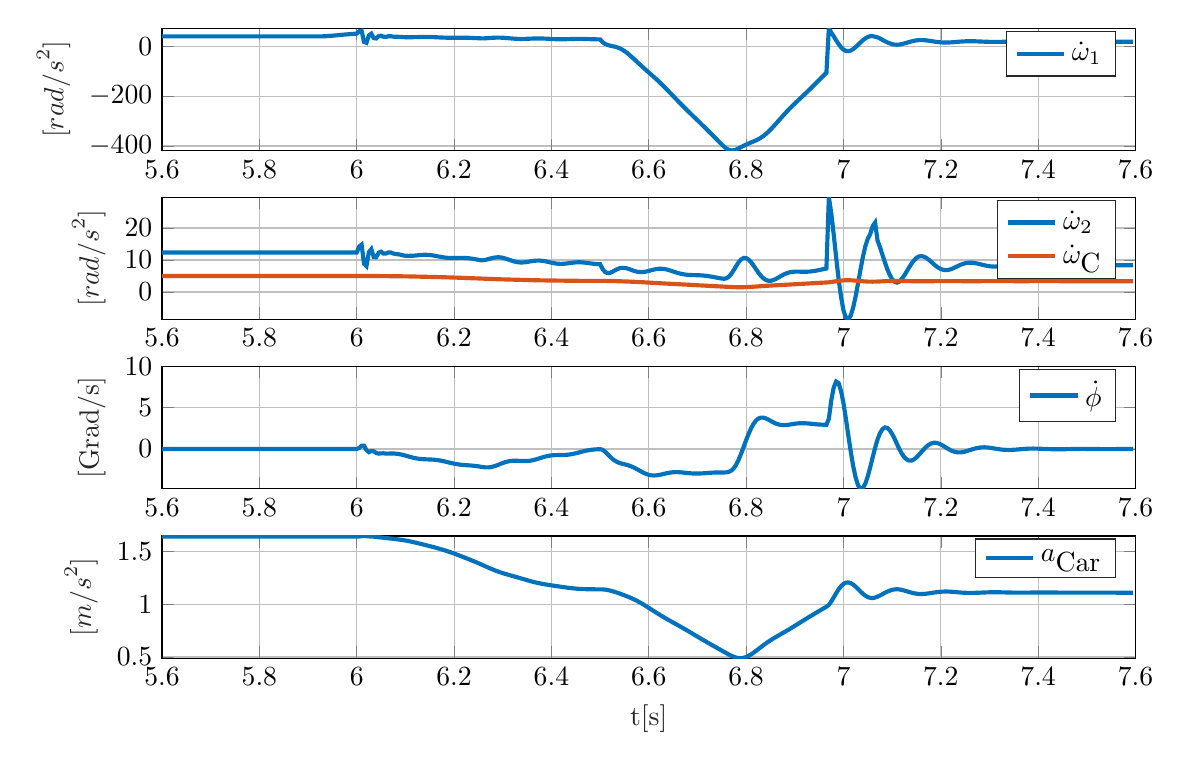
\begin{tikzpicture}

\begin{axis}[%
width=0.951\awidth,
height=0.194\aheight,
at={(0\awidth,0.806\aheight)},
scale only axis,
xmin=5.6,
xmax=7.6,
ymin=-417.664429354826,
ymax=72.7935981722241,
ylabel style={font=\color{white!15!black}},
ylabel={$\text{[rad/s}^\text{2}\text{]}$},
axis background/.style={fill=white},
xmajorgrids,
ymajorgrids,
legend style={legend cell align=left, align=left, draw=white!15!black}
]
\addplot [color=mycolor1, line width=1.5pt]
  table[row sep=crcr]{%
5.6	40.0360858533288\\
5.605	40.0361167967789\\
5.61	40.0361477133084\\
5.615	40.03617857401\\
5.62	40.0362094052232\\
5.625	40.0362401793584\\
5.63	40.0362709254895\\
5.635	40.0363016146811\\
5.64	40.0363322760286\\
5.645	40.0363628819075\\
5.65	40.0363934574151\\
5.655	40.0364239789503\\
5.66	40.0364544702514\\
5.665	40.0364849090093\\
5.67	40.0365153177049\\
5.675	40.0365456699484\\
5.68	40.0365759949108\\
5.685	40.0366062649342\\
5.69	40.0366365051229\\
5.695	40.0366666932176\\
5.7	40.0366968502741\\
5.705	40.0367725377863\\
5.71	40.0368389815492\\
5.715	40.0368886915464\\
5.72	40.0369193437496\\
5.725	40.0369377436488\\
5.73	40.0369543093394\\
5.735	40.036976489991\\
5.74	40.0370079553001\\
5.745	40.037047946015\\
5.75	40.0370926799768\\
5.755	40.0371385365792\\
5.76	40.0371821969765\\
5.765	40.0372226340834\\
5.77	40.0372601222993\\
5.775	40.0372961629141\\
5.78	40.0373325359807\\
5.785	40.0373708980486\\
5.79	40.0374122057864\\
5.795	40.0374570921719\\
5.8	40.0375053228833\\
5.805	40.0375568897206\\
5.81	40.0376112023581\\
5.815	40.0376683843832\\
5.82	40.0377282321123\\
5.825	40.0377914265074\\
5.83	40.0378583497105\\
5.835	40.0379302821816\\
5.84	40.0380080800697\\
5.845	40.0380935843313\\
5.85	40.038188058351\\
5.855	40.0382939944229\\
5.86	40.0384132169747\\
5.865	40.0385492177053\\
5.87	40.0387048051699\\
5.875	40.0388851210481\\
5.88	40.0390947114709\\
5.885	40.0393414483438\\
5.89	40.0396328332936\\
5.895	40.0399812167225\\
5.9	40.0419891033533\\
5.905	40.0459799738722\\
5.91	40.0496862898839\\
5.915	40.0536638093024\\
5.92	40.0592679568223\\
5.925	40.0685653831155\\
5.93	40.232866151909\\
5.935	40.6353960123335\\
5.94	41.2281492874086\\
5.945	41.9938412863546\\
5.95	42.8921612973889\\
5.955	43.6199502756565\\
5.96	44.5416408480299\\
5.965	45.5368451993716\\
5.97	46.4829310754561\\
5.975	47.3429215077385\\
5.98	48.1735020725965\\
5.985	48.9403023026508\\
5.99	49.5943567930395\\
5.995	50.4968568911064\\
6	51.2419538044049\\
6.005	60.3548929307732\\
6.01	62.6430650601239\\
6.015	18.1040280415948\\
6.02	14.3207707231346\\
6.025	44.09814406618\\
6.03	50.9879267682384\\
6.035	33.0794596566776\\
6.04	31.7251417269782\\
6.045	40.831678793929\\
6.05	42.9097522193509\\
6.055	38.5510416260345\\
6.06	38.0764487106552\\
6.065	40.4692599804846\\
6.07	40.6097100777422\\
6.075	38.938438145849\\
6.08	38.2665563727247\\
6.085	38.3469495379708\\
6.09	38.0198773761417\\
6.095	37.1887431247787\\
6.1	36.7279010615086\\
6.105	36.7323304976569\\
6.11	36.8232294671168\\
6.115	36.8416603227803\\
6.12	36.99004465219\\
6.125	37.2957784027737\\
6.13	37.5899689829282\\
6.135	37.7581516608303\\
6.14	37.8086532555277\\
6.145	37.7644903631247\\
6.15	37.5949025159786\\
6.155	37.2752736600746\\
6.16	36.8463522011887\\
6.165	36.3727497932095\\
6.17	35.8951811947805\\
6.175	35.443555279128\\
6.18	35.0613112954622\\
6.185	34.7826396534103\\
6.19	34.6134263180862\\
6.195	34.5409618504778\\
6.2	34.5459773316727\\
6.205	34.5988357823936\\
6.21	34.6595867212722\\
6.215	34.6880700183987\\
6.22	34.6524726989589\\
6.225	34.5308311427872\\
6.23	34.311798451696\\
6.235	33.998351279928\\
6.24	33.606822538989\\
6.245	33.1631580430518\\
6.25	32.6982601079238\\
6.255	32.2219357723467\\
6.26	32.0996475444554\\
6.265	32.475898056796\\
6.27	33.2433752879054\\
6.275	33.9623832864166\\
6.28	34.4852943926882\\
6.285	34.8975650980135\\
6.29	35.1264544107583\\
6.295	35.0319798230813\\
6.3	34.5763711157459\\
6.305	33.868350298903\\
6.31	33.024719619115\\
6.315	32.1722262435617\\
6.32	31.3671831407275\\
6.325	30.649947515688\\
6.33	30.1130854580637\\
6.335	29.8355419155659\\
6.34	29.8203075831594\\
6.345	30.0069257611115\\
6.35	30.3400355033562\\
6.355	30.7674791733117\\
6.36	31.2019947410255\\
6.365	31.5457554109754\\
6.37	31.7382124307706\\
6.375	31.7512524943599\\
6.38	31.572075906294\\
6.385	31.2107842812372\\
6.39	30.7135585698787\\
6.395	30.1470536770896\\
6.4	29.5794433203569\\
6.405	29.0745378604326\\
6.41	28.6893151528192\\
6.415	28.4630285978042\\
6.42	28.4091285415751\\
6.425	28.5141566900316\\
6.43	28.7465228196674\\
6.435	29.0590015339313\\
6.44	29.3939089648807\\
6.445	29.6936890451346\\
6.45	29.9102206775099\\
6.455	30.0101718597564\\
6.46	29.9783423290311\\
6.465	29.8196131926887\\
6.47	29.5579629080018\\
6.475	29.2316371226142\\
6.48	28.886690462414\\
6.485	28.5704180052266\\
6.49	28.3247489381814\\
6.495	28.1802495018807\\
6.5	28.1483029334591\\
6.505	17.5089482304227\\
6.51	10.1809140219622\\
6.515	5.72760532039593\\
6.52	2.97464603943853\\
6.525	0.988400792000554\\
6.53	-1.07678086005585\\
6.535	-3.81385455884178\\
6.54	-7.58445316186751\\
6.545	-12.5500704588089\\
6.55	-18.6503604950521\\
6.555	-25.7897830894559\\
6.56	-33.7760151701105\\
6.565	-42.3651991174332\\
6.57	-51.3176811741372\\
6.575	-60.422510448769\\
6.58	-69.521006628096\\
6.585	-78.5129843848206\\
6.59	-87.3583181207979\\
6.595	-96.0687468223414\\
6.6	-104.695106841566\\
6.605	-113.314657289094\\
6.61	-122.012267370453\\
6.615	-130.866702664061\\
6.62	-139.938773974937\\
6.625	-149.263745096454\\
6.63	-158.84823564019\\
6.635	-168.670571506867\\
6.64	-178.685968677258\\
6.645	-188.833451432688\\
6.65	-199.044484763492\\
6.655	-209.25152549\\
6.66	-219.395781753006\\
6.665	-229.432868692206\\
6.67	-239.336670853\\
6.675	-249.100094184509\\
6.68	-258.733668638872\\
6.685	-268.262170673927\\
6.69	-277.719992440156\\
6.695	-287.145771714393\\
6.7	-296.577226883947\\
6.705	-306.046656127542\\
6.71	-315.577579989834\\
6.715	-325.183051566266\\
6.72	-334.86557558142\\
6.725	-344.617360755384\\
6.73	-354.423074826757\\
6.735	-364.262551881089\\
6.74	-374.1138859636\\
6.745	-383.956266528427\\
6.75	-393.772425804402\\
6.755	-403.123231549089\\
6.76	-410.800481912981\\
6.765	-415.751950579352\\
6.77	-417.664429354826\\
6.775	-416.777017183334\\
6.78	-413.66710297143\\
6.785	-409.047512448918\\
6.79	-403.89660669851\\
6.795	-398.827568654643\\
6.8	-394.101514661699\\
6.805	-389.769483302399\\
6.81	-385.717587676769\\
6.815	-381.712185595134\\
6.82	-377.453348804041\\
6.825	-372.641609107635\\
6.83	-367.019324904296\\
6.835	-360.415252910424\\
6.84	-352.753570030764\\
6.845	-344.064978655367\\
6.85	-334.46553345199\\
6.855	-324.142091420937\\
6.86	-313.316897657585\\
6.865	-302.224534872852\\
6.87	-291.080195016906\\
6.875	-280.063803774385\\
6.88	-269.3028967871\\
6.885	-258.871403800544\\
6.89	-248.788136160247\\
6.895	-239.028698382228\\
6.9	-229.533284382815\\
6.905	-220.224737068881\\
6.91	-211.017188005327\\
6.915	-201.832744044196\\
6.92	-192.604832083184\\
6.925	-183.289008086685\\
6.93	-173.859179979382\\
6.935	-164.31208397128\\
6.94	-154.65826646365\\
6.945	-144.922696006766\\
6.95	-135.134027199155\\
6.955	-125.324677451451\\
6.96	-115.521426023419\\
6.965	-105.747386552451\\
6.97	72.7935981722241\\
6.975	55.4490355286459\\
6.98	40.3570579372353\\
6.985	24.2915230077808\\
6.99	9.11408473507417\\
6.995	-3.42662584658651\\
7	-13.0239592951734\\
7.005	-18.1872441341329\\
7.01	-19.3404925384138\\
7.015	-16.6889527009767\\
7.02	-11.0105208144504\\
7.025	-3.11424705176506\\
7.03	6.16826053337161\\
7.035	15.7868979706506\\
7.04	24.7814786364631\\
7.045	32.2320760275818\\
7.05	37.6297770458922\\
7.055	40.820264080916\\
7.06	41.1003733350938\\
7.065	38.6224766006298\\
7.07	36.3589383896286\\
7.075	31.6231175099223\\
7.08	26.3440358639844\\
7.085	21.0085465382988\\
7.09	16.1380069003845\\
7.095	12.0808811153089\\
7.1	8.98184173512114\\
7.105	7.12468202868895\\
7.11	6.570887215061\\
7.115	7.30649642987423\\
7.12	9.18947793882977\\
7.125	11.6844788889662\\
7.13	14.5015608044958\\
7.135	17.3660884339009\\
7.14	20.0452529890494\\
7.145	22.3027628559804\\
7.15	23.9988607268995\\
7.155	25.0182774083109\\
7.16	25.2800916870647\\
7.165	24.908770080892\\
7.17	24.047335752355\\
7.175	22.7926186412323\\
7.18	21.2994658683349\\
7.185	19.7453832864745\\
7.19	18.2866230370118\\
7.195	17.0638693081657\\
7.2	16.1596419223441\\
7.205	15.5866686300489\\
7.21	15.3541465873902\\
7.215	15.4927795470353\\
7.22	15.9493759444849\\
7.225	16.6247882334145\\
7.23	17.4305507466018\\
7.235	18.2694993052992\\
7.24	19.0598426359936\\
7.245	19.7227029140721\\
7.25	20.2105493199646\\
7.255	20.5094778051407\\
7.26	20.6258603028903\\
7.265	20.5588528465663\\
7.27	20.3456201130802\\
7.275	20.0134490611162\\
7.28	19.6074093382443\\
7.285	19.1760056778217\\
7.29	18.7655090159797\\
7.295	18.4053853975552\\
7.3	18.1262643595601\\
7.305	17.9456802877935\\
7.31	17.8738179413238\\
7.315	17.8971908869612\\
7.32	17.9976064794883\\
7.325	18.1709601378841\\
7.33	18.3802663883963\\
7.335	18.6004949816797\\
7.34	18.8130589256284\\
7.345	19.0027360176271\\
7.35	19.1527671815719\\
7.355	19.253572122846\\
7.36	19.300857531026\\
7.365	19.2962946978867\\
7.37	19.2481357620555\\
7.375	19.1629406436358\\
7.38	19.0547511583149\\
7.385	18.936991237992\\
7.39	18.822901784833\\
7.395	18.7226011257744\\
7.4	18.6415171781358\\
7.405	18.5862060385378\\
7.41	18.5567338275052\\
7.415	18.5545577016108\\
7.42	18.5772426668011\\
7.425	18.6180595837293\\
7.43	18.6713560392215\\
7.435	18.7304984658882\\
7.44	18.789212925478\\
7.445	18.8420475645623\\
7.45	18.8847491838125\\
7.455	18.9145409240724\\
7.46	18.9301745007437\\
7.465	18.9318667103923\\
7.47	18.9210288489207\\
7.475	18.9003926657898\\
7.48	18.8729044860584\\
7.485	18.8419085545726\\
7.49	18.8106628173421\\
7.495	18.7820526054459\\
7.5	18.7583641781635\\
7.505	18.7411401537771\\
7.51	18.7311399972217\\
7.515	18.7283477126188\\
7.52	18.7322717407003\\
7.525	18.7412421016728\\
7.53	18.7540427779343\\
7.535	18.7689298997312\\
7.54	18.7841732475995\\
7.545	18.7982669270957\\
7.55	18.8099898515226\\
7.555	18.8184878094577\\
7.56	18.8233100219747\\
7.565	18.8244024405326\\
7.57	18.8220401929987\\
7.575	18.8168807852129\\
7.58	18.809644979756\\
7.585	18.8012411545069\\
7.59	18.7925202258166\\
7.595	18.7842792731393\\
};
\addlegendentry{$\dot{\omega}_1$}

\end{axis}

\begin{axis}[%
width=0.951\awidth,
height=0.194\aheight,
at={(0\awidth,0.538\aheight)},
scale only axis,
xmin=5.6,
xmax=7.6,
ymin=-8.5245297968645,
ymax=29.6692322538102,
ylabel style={font=\color{white!15!black}},
ylabel={$\text{[rad/s}^\text{2}\text{]}$},
axis background/.style={fill=white},
xmajorgrids,
ymajorgrids,
legend style={legend cell align=left, align=left, draw=white!15!black}
]
\addplot [color=mycolor1, line width=1.5pt]
  table[row sep=crcr]{%
5.6	12.3444588354187\\
5.605	12.3444683767812\\
5.61	12.3444779079146\\
5.615	12.3444874224415\\
5.62	12.3444969272841\\
5.625	12.344506415765\\
5.63	12.3445158941058\\
5.635	12.3445253565951\\
5.64	12.3445348090881\\
5.645	12.3445442450884\\
5.65	12.3445536715308\\
5.655	12.3445630817832\\
5.66	12.3445724822413\\
5.665	12.344581866344\\
5.67	12.3445912408806\\
5.675	12.3446005995129\\
5.68	12.3446099481989\\
5.685	12.3446192807314\\
5.69	12.3446286041335\\
5.695	12.344637911011\\
5.7	12.3446472086207\\
5.705	12.3446543387417\\
5.71	12.3446628475904\\
5.715	12.3446726798875\\
5.72	12.3446831894189\\
5.725	12.3446936725295\\
5.73	12.3447036253528\\
5.735	12.3447128954458\\
5.74	12.3447216500326\\
5.745	12.34473016027\\
5.75	12.3447387057213\\
5.755	12.3447474622026\\
5.76	12.3447564499493\\
5.765	12.3447656387661\\
5.77	12.3447748977787\\
5.775	12.3447841475872\\
5.78	12.3447933013786\\
5.785	12.3448023457959\\
5.79	12.3448112709584\\
5.795	12.3448201235533\\
5.8	12.3448289077278\\
5.805	12.344837683605\\
5.81	12.3448464160001\\
5.815	12.3448551611837\\
5.82	12.3448638376203\\
5.825	12.344872506259\\
5.83	12.3448810540604\\
5.835	12.3448895637202\\
5.84	12.3448978957367\\
5.845	12.3449061665133\\
5.85	12.3449141936326\\
5.855	12.3449221385972\\
5.86	12.34492974358\\
5.865	12.3449372290052\\
5.87	12.3449442178817\\
5.875	12.3449510132168\\
5.88	12.3449570555795\\
5.885	12.3449627696727\\
5.89	12.3449673185223\\
5.895	12.3449713083546\\
5.9	12.3449980614541\\
5.905	12.3449940346036\\
5.91	12.3449950609765\\
5.915	12.3449998648175\\
5.92	12.3450028418229\\
5.925	12.3449956584336\\
5.93	12.3442033394522\\
5.935	12.3427046475599\\
5.94	12.3408099046856\\
5.945	12.3389536315308\\
5.95	12.3375953442664\\
5.955	12.3381881296618\\
5.96	12.3389396264756\\
5.965	12.3403753866623\\
5.97	12.3428967070286\\
5.975	12.34546044325\\
5.98	12.3483961178699\\
5.985	12.3494930806846\\
5.99	12.3487623763267\\
5.995	12.3523653839411\\
6	12.3500959337398\\
6.005	14.1829961148815\\
6.01	14.8048461703502\\
6.015	8.8613618363288\\
6.02	8.10737840965794\\
6.025	12.4661903562728\\
6.03	13.3903772475223\\
6.035	10.9127039291207\\
6.04	10.8590356972772\\
6.045	12.2497623763502\\
6.05	12.5975677383449\\
6.055	12.0364211581391\\
6.06	12.0111451566081\\
6.065	12.3511702828064\\
6.07	12.3334891947288\\
6.075	12.0317617925393\\
6.08	11.8575348822242\\
6.085	11.779912850584\\
6.09	11.643602697206\\
6.095	11.4480747450771\\
6.1	11.3277245654908\\
6.105	11.2982907081869\\
6.11	11.3058848713163\\
6.115	11.325951052886\\
6.12	11.3816045713693\\
6.125	11.4674283715794\\
6.13	11.5500470870547\\
6.135	11.6051833466754\\
6.14	11.626532219123\\
6.145	11.6130209008161\\
6.15	11.5587473257056\\
6.155	11.4618781672189\\
6.16	11.3329120727631\\
6.165	11.1877133529169\\
6.17	11.0396656468656\\
6.175	10.9006126319537\\
6.18	10.7830643711704\\
6.185	10.6961736130106\\
6.19	10.6424328604062\\
6.195	10.6190452740238\\
6.2	10.6198073249943\\
6.205	10.6352263857289\\
6.21	10.6533441844658\\
6.215	10.6621207474586\\
6.22	10.6515785970951\\
6.225	10.6147185386772\\
6.23	10.5480223057002\\
6.235	10.4523885315057\\
6.24	10.3326340068152\\
6.245	10.1965713985874\\
6.25	10.0536816108024\\
6.255	9.9394237897468\\
6.26	9.93999491671912\\
6.265	10.0599507177844\\
6.27	10.2692538141096\\
6.275	10.4827591320868\\
6.28	10.6589150579725\\
6.285	10.7911836712155\\
6.29	10.8554914525525\\
6.295	10.8249600591776\\
6.3	10.6909234959626\\
6.305	10.4769902517946\\
6.31	10.2250859099536\\
6.315	9.96125615002302\\
6.32	9.70793888091475\\
6.325	9.48715378686711\\
6.33	9.32407605769367\\
6.335	9.23660105894578\\
6.34	9.22663514882743\\
6.345	9.28142592350923\\
6.35	9.38399056148728\\
6.355	9.51446349703019\\
6.36	9.64636180980688\\
6.365	9.75258198283609\\
6.37	9.81391532233602\\
6.375	9.8196584328989\\
6.38	9.76571605443132\\
6.385	9.65646314613832\\
6.39	9.50543543033882\\
6.395	9.33206615277322\\
6.4	9.15741097341606\\
6.405	9.00169484425714\\
6.41	8.88237866115696\\
6.415	8.81127918955008\\
6.42	8.79282303441005\\
6.425	8.82351850884106\\
6.43	8.89369495117353\\
6.435	8.98880357013422\\
6.44	9.09133340474682\\
6.445	9.18372925804988\\
6.45	9.2510597551136\\
6.455	9.28286342275078\\
6.46	9.27433797177764\\
6.465	9.22684012213131\\
6.47	9.14751766899917\\
6.475	9.04793981137345\\
6.48	8.94219260609998\\
6.485	8.84481298940864\\
6.49	8.76871579272256\\
6.495	8.72338032138578\\
6.5	8.71424852556947\\
6.505	7.21850891292888\\
6.51	6.2697045073578\\
6.515	5.90558780000902\\
6.52	5.96550103331992\\
6.525	6.29169538754059\\
6.53	6.71957381954871\\
6.535	7.12119050471028\\
6.54	7.4109245185341\\
6.545	7.54706683078621\\
6.55	7.53211260974285\\
6.555	7.38445004645882\\
6.56	7.14452337599232\\
6.565	6.86416984393691\\
6.57	6.59417780503418\\
6.575	6.37773307889938\\
6.58	6.24409142288823\\
6.585	6.2069021622392\\
6.59	6.26389551672401\\
6.595	6.39930174327583\\
6.6	6.58755705307522\\
6.605	6.79711070465373\\
6.61	6.99582082947791\\
6.615	7.15489559346952\\
6.62	7.25228647627955\\
6.625	7.27474851280658\\
6.63	7.21857111135523\\
6.635	7.08929136446886\\
6.64	6.8999365506379\\
6.645	6.66879076312352\\
6.65	6.41666103563739\\
6.655	6.16419848306214\\
6.66	5.92948392771814\\
6.665	5.72626796174336\\
6.67	5.56277561143725\\
6.675	5.44145848760354\\
6.68	5.35940688170058\\
6.685	5.30936326546589\\
6.69	5.28111589360469\\
6.695	5.26311638848983\\
6.7	5.24403527138156\\
6.705	5.2141193059897\\
6.71	5.16620486221655\\
6.715	5.09623472995281\\
6.72	5.00328873551007\\
6.725	4.88952282903574\\
6.73	4.75935577352902\\
6.735	4.61867125015397\\
6.74	4.47390233151236\\
6.745	4.33119267979555\\
6.75	4.19567152622949\\
6.755	4.13235974844974\\
6.76	4.3077500482068\\
6.765	4.85220678592214\\
6.77	5.7654401157979\\
6.775	6.94149274281699\\
6.78	8.21678725450056\\
6.785	9.37608590325453\\
6.79	10.2074714488926\\
6.795	10.6181687403769\\
6.8	10.5818953127932\\
6.805	10.1325545340223\\
6.81	9.34417434728584\\
6.815	8.32636232975119\\
6.82	7.20387863460337\\
6.825	6.09866937432525\\
6.83	5.11637136931404\\
6.835	4.33496904161711\\
6.84	3.80073398238164\\
6.845	3.52632627127605\\
6.85	3.49566677148096\\
6.855	3.6691973141028\\
6.86	3.993262679292\\
6.865	4.40772274689698\\
6.87	4.85472110295905\\
6.875	5.28427445595798\\
6.88	5.65913871022212\\
6.885	5.95626441087461\\
6.89	6.1672128856485\\
6.895	6.29585985196354\\
6.9	6.35593587255835\\
6.905	6.3668858001447\\
6.91	6.35085115329957\\
6.915	6.3287777762871\\
6.92	6.31863537082199\\
6.925	6.33306440958313\\
6.93	6.37948731638926\\
6.935	6.45948011390556\\
6.94	6.57038233959429\\
6.945	6.7057614869027\\
6.95	6.85760819362486\\
6.955	7.01699843293409\\
6.96	7.17601999477392\\
6.965	7.32795805653541\\
6.97	29.6692322538102\\
6.975	24.5528073362093\\
6.98	17.9109918879772\\
6.985	10.8026592285232\\
6.99	4.08266603754282\\
6.995	-1.46569734414061\\
7	-5.71970214842713\\
7.005	-8.00838738765106\\
7.01	-8.5245297968645\\
7.015	-7.36400038753845\\
7.02	-4.85308975885573\\
7.025	-1.35835041081191\\
7.03	2.74639739664053\\
7.035	7.00672489733824\\
7.04	10.9884304861698\\
7.045	14.318142390197\\
7.05	16.6642355437953\\
7.055	18.1001931741162\\
7.06	20.5777464011639\\
7.065	21.6655312753091\\
7.07	16.1200928717917\\
7.075	14.0263373527714\\
7.08	11.6911712284732\\
7.085	9.33081959175706\\
7.09	7.17565299014541\\
7.095	5.37990180292763\\
7.1	4.00726697109303\\
7.105	3.18410446235339\\
7.11	2.93742952012008\\
7.115	3.24717871414532\\
7.12	4.12953322045405\\
7.125	5.19650380090934\\
7.13	6.43493815767988\\
7.135	7.70538620777506\\
7.14	8.89522055801172\\
7.145	9.89365592759805\\
7.15	10.6457826045248\\
7.155	11.0987866647356\\
7.16	11.2155369806887\\
7.165	11.0432573093481\\
7.17	10.6698416920908\\
7.175	10.1152719980673\\
7.18	9.45493281626887\\
7.185	8.76745842307128\\
7.19	8.12196137520959\\
7.195	7.58070041178416\\
7.2	7.18030646763236\\
7.205	6.92634427326902\\
7.21	6.82297433391113\\
7.215	6.88329728651979\\
7.22	7.08429820438414\\
7.225	7.38326319371708\\
7.23	7.73964247535696\\
7.235	8.1102117055857\\
7.24	8.46105848971592\\
7.245	8.75474021696073\\
7.25	8.97074542082964\\
7.255	9.10366193822529\\
7.26	9.15524363006398\\
7.265	9.12422733785797\\
7.27	9.03131148452167\\
7.275	8.88450663073263\\
7.28	8.70494989577674\\
7.285	8.51412910217641\\
7.29	8.33249134242897\\
7.295	8.17310124372352\\
7.3	8.04950902381688\\
7.305	7.96950362517646\\
7.31	7.93756549922909\\
7.315	7.95590906922962\\
7.32	7.98855629589252\\
7.325	8.07947308613029\\
7.33	8.16277155623493\\
7.335	8.25615847869267\\
7.34	8.35247779343399\\
7.345	8.4368578114063\\
7.35	8.50304376057466\\
7.355	8.54786997565134\\
7.36	8.56886856008668\\
7.365	8.56644253926652\\
7.37	8.54554356885183\\
7.375	8.50789666870196\\
7.38	8.46005645008654\\
7.385	8.4079684443991\\
7.39	8.35749194242908\\
7.395	8.31310315857672\\
7.4	8.27720029149714\\
7.405	8.25270007861582\\
7.41	8.23962418096289\\
7.415	8.23868010082106\\
7.42	8.24804540357718\\
7.425	8.26659650314559\\
7.43	8.29017168870996\\
7.435	8.31627656807541\\
7.44	8.34230142362048\\
7.445	8.36572118157437\\
7.45	8.38465221826755\\
7.455	8.39787297024895\\
7.46	8.40482685407051\\
7.465	8.40575098520958\\
7.47	8.4007673030078\\
7.475	8.39164006131796\\
7.48	8.37948687177686\\
7.485	8.36577748017407\\
7.49	8.35195354346843\\
7.495	8.33929192553387\\
7.5	8.32880484599673\\
7.505	8.32117577626195\\
7.51	8.31674157418547\\
7.515	8.31549629623805\\
7.52	8.3168413384642\\
7.525	8.3210289975118\\
7.53	8.32688865089403\\
7.535	8.33340254158065\\
7.54	8.34013727326146\\
7.545	8.34639568288821\\
7.55	8.35159227266558\\
7.555	8.35535993904296\\
7.56	8.35750327783217\\
7.565	8.35803028306054\\
7.57	8.35693809393933\\
7.575	8.35465589452906\\
7.58	8.35145661180104\\
7.585	8.34773904679787\\
7.59	8.34388033050072\\
7.595	8.34023293779182\\
};
\addlegendentry{$\dot{\omega}_2$}

\addplot [color=mycolor2, line width=1.5pt]
  table[row sep=crcr]{%
5.6	4.99774050300873\\
5.605	4.99774436418014\\
5.61	4.99774822005694\\
5.615	4.99775207056964\\
5.62	4.99775591580554\\
5.625	4.99775975569511\\
5.63	4.9977635903256\\
5.635	4.9977674196274\\
5.64	4.99777124368777\\
5.645	4.99777506243702\\
5.65	4.99777887596238\\
5.655	4.99778268419413\\
5.66	4.99778648721948\\
5.665	4.99779028496863\\
5.67	4.99779407752882\\
5.675	4.99779786483016\\
5.68	4.99780164695987\\
5.685	4.99780542384805\\
5.69	4.99780919558184\\
5.695	4.9978129620913\\
5.7	4.99781672346361\\
5.705	4.99782047993657\\
5.71	4.99782423033098\\
5.715	4.99782797505723\\
5.72	4.99783171435639\\
5.725	4.99783544844636\\
5.73	4.99783917772615\\
5.735	4.99784290235644\\
5.74	4.99784662251659\\
5.745	4.99785033807247\\
5.75	4.99785404893247\\
5.755	4.99785775479194\\
5.76	4.99786145550339\\
5.765	4.99786515081759\\
5.77	4.99786884071231\\
5.775	4.9978725250923\\
5.78	4.9978762040824\\
5.785	4.99787987770012\\
5.79	4.99788354613933\\
5.795	4.99788720944145\\
5.8	4.99789086778475\\
5.805	4.99789452116845\\
5.81	4.99789816970918\\
5.815	4.99790181333974\\
5.82	4.99790545210924\\
5.825	4.99790908589318\\
5.83	4.99791271469319\\
5.835	4.9979163383548\\
5.84	4.99791995686182\\
5.845	4.99792357005976\\
5.85	4.99792717793828\\
5.855	4.99793078036022\\
5.86	4.99793437732552\\
5.865	4.99793796870897\\
5.87	4.9979415544989\\
5.875	4.99794513455144\\
5.88	4.99794870879685\\
5.885	4.99795227702232\\
5.89	4.9979558390345\\
5.895	4.99795939448818\\
5.9	4.9979629300282\\
5.905	4.99796641874142\\
5.91	4.99796984923823\\
5.915	4.99797321741982\\
5.92	4.99797651898027\\
5.925	4.99797973502694\\
5.93	4.99798197887247\\
5.935	4.99798072592283\\
5.94	4.99797291168771\\
5.945	4.99795523614734\\
5.95	4.99792525100562\\
5.955	4.9978835142187\\
5.96	4.997832196419\\
5.965	4.99777367393949\\
5.97	4.99771180023199\\
5.975	4.99765176528473\\
5.98	4.99759883465355\\
5.985	4.9975584187722\\
5.99	4.99753210740251\\
5.995	4.9975190274204\\
6	4.99751741287588\\
6.005	4.99977639561069\\
6.01	5.00685362198219\\
6.015	5.01362702794096\\
6.02	5.0078761661919\\
6.025	5.00009133597546\\
6.03	4.99735133800362\\
6.035	4.99340664937259\\
6.04	4.9853283058232\\
6.045	4.97656793500899\\
6.05	4.96933390220487\\
6.055	4.96206481411845\\
6.06	4.95401823297508\\
6.065	4.94604207957095\\
6.07	4.93858006904639\\
6.075	4.93100859316804\\
6.08	4.92284131954094\\
6.085	4.91405376092315\\
6.09	4.90454356255745\\
6.095	4.89402624023015\\
6.1	4.88226174835254\\
6.105	4.86926884551148\\
6.11	4.85514208425963\\
6.115	4.83998298062429\\
6.12	4.82393308117649\\
6.125	4.80721671158169\\
6.13	4.79005012241079\\
6.135	4.77259471116174\\
6.14	4.75497005519955\\
6.145	4.73722220332332\\
6.15	4.71934014624177\\
6.155	4.70124149559751\\
6.16	4.68278408969681\\
6.165	4.66379749509135\\
6.17	4.64411113485623\\
6.175	4.62357301589524\\
6.18	4.60207088734504\\
6.185	4.57954748309131\\
6.19	4.55600932394165\\
6.195	4.53151877609335\\
6.2	4.50618398657522\\
6.205	4.48014129895679\\
6.21	4.45353528556462\\
6.215	4.42649673918224\\
6.22	4.39912435874352\\
6.225	4.37147326103143\\
6.23	4.34355090285911\\
6.235	4.31531284393891\\
6.24	4.28667585307695\\
6.245	4.2575302021046\\
6.25	4.22775663027701\\
6.255	4.1971884920865\\
6.26	4.16598596625721\\
6.265	4.13454475113008\\
6.27	4.10326955843197\\
6.275	4.07268563693346\\
6.28	4.04322161896892\\
6.285	4.01521588091507\\
6.29	3.98888323227646\\
6.295	3.96428471230602\\
6.3	3.94138340386602\\
6.305	3.91985603372114\\
6.31	3.89915729959542\\
6.315	3.87907156362929\\
6.32	3.85927037326069\\
6.325	3.83945211119474\\
6.33	3.81942183611667\\
6.335	3.79911085808592\\
6.34	3.77857935219684\\
6.345	3.75800402125431\\
6.35	3.73764621501273\\
6.355	3.71781039763425\\
6.36	3.6988074023068\\
6.365	3.68089947525348\\
6.37	3.66426377095242\\
6.375	3.64897675965497\\
6.38	3.63501228870667\\
6.385	3.6222375573656\\
6.39	3.61044418719348\\
6.395	3.59938139891513\\
6.4	3.58879353988988\\
6.405	3.57845603097584\\
6.41	3.56820456863425\\
6.415	3.5579583927722\\
6.42	3.54772391972407\\
6.425	3.537596544927\\
6.43	3.52773745177536\\
6.435	3.51834881859275\\
6.44	3.50964439598866\\
6.445	3.50181767096956\\
6.45	3.49501489513242\\
6.455	3.48931701720363\\
6.46	3.48473088828519\\
6.465	3.48119189849735\\
6.47	3.47857599213195\\
6.475	3.47672041967086\\
6.48	3.47544866761355\\
6.485	3.47459618355126\\
6.49	3.47403334611672\\
6.495	3.47368254546691\\
6.5	3.47352490849553\\
6.505	3.4717855642655\\
6.51	3.46597618545572\\
6.515	3.455468199411\\
6.52	3.44065623214126\\
6.525	3.42216574862908\\
6.53	3.40088928818346\\
6.535	3.37765574465768\\
6.54	3.35309785277773\\
6.545	3.32752986525616\\
6.55	3.30105122203202\\
6.555	3.27352621726011\\
6.56	3.24464582091836\\
6.565	3.21404128413653\\
6.57	3.18137356541213\\
6.575	3.14639869701559\\
6.58	3.10903354168806\\
6.585	3.06936924607156\\
6.59	3.02767053100919\\
6.595	2.98434330336112\\
6.6	2.93988802528569\\
6.605	2.89485018873535\\
6.61	2.84975489419771\\
6.615	2.80505917627652\\
6.62	2.76111128077592\\
6.625	2.71812797875858\\
6.63	2.67618857556491\\
6.635	2.63524162892292\\
6.64	2.59513078591181\\
6.645	2.55562590966536\\
6.65	2.51646033752059\\
6.655	2.47736690568093\\
6.66	2.4381101136566\\
6.665	2.39850955064197\\
6.67	2.35845567152161\\
6.675	2.3179132489012\\
6.68	2.27691617906193\\
6.685	2.23555451795476\\
6.69	2.19395663064224\\
6.695	2.15226848666149\\
6.7	2.1106337863747\\
6.705	2.06917663352773\\
6.71	2.02798862740612\\
6.715	1.98712224919342\\
6.72	1.94659047139259\\
6.725	1.9063674421966\\
6.73	1.86639871571268\\
6.735	1.82661125197817\\
6.74	1.78692489772278\\
6.745	1.74726287101909\\
6.75	1.70756081470081\\
6.755	1.66781445576045\\
6.76	1.62836814201842\\
6.765	1.59020766590382\\
6.77	1.55495562345558\\
6.775	1.5247767193652\\
6.78	1.50187791663144\\
6.785	1.48927646563348\\
6.79	1.48861980656842\\
6.795	1.4997176694874\\
6.8	1.52209813620012\\
6.805	1.55455287343866\\
6.81	1.59550027968291\\
6.815	1.64290701917578\\
6.82	1.69461720077496\\
6.825	1.74855808940493\\
6.83	1.80292484502514\\
6.835	1.85629915573517\\
6.84	1.90771494142812\\
6.845	1.95666391228893\\
6.85	2.00304958990867\\
6.855	2.04710931433761\\
6.86	2.08930931777422\\
6.865	2.13024004572175\\
6.87	2.17051383479636\\
6.875	2.21068444477467\\
6.88	2.25118834165616\\
6.885	2.2923130244665\\
6.89	2.33419118298582\\
6.895	2.37681378051216\\
6.9	2.42006090195833\\
6.905	2.4637379552978\\
6.91	2.50761694497598\\
6.915	2.55147171311129\\
6.92	2.59510801036282\\
6.925	2.63838248067999\\
6.93	2.68121232555464\\
6.935	2.72357515155301\\
6.94	2.76550118040468\\
6.945	2.80706046867573\\
6.95	2.84834727712483\\
6.955	2.88946445798955\\
6.96	2.93050972854744\\
6.965	2.97156486406472\\
6.97	3.02418384111007\\
6.975	3.12513824709721\\
6.98	3.24121673916359\\
6.985	3.36151475356012\\
6.99	3.47250920090417\\
6.995	3.56254235662688\\
7	3.63052296574211\\
7.005	3.66597951538666\\
7.01	3.67248522535902\\
7.015	3.65163099149097\\
7.02	3.60903811192541\\
7.025	3.55056578412548\\
7.03	3.48223588418768\\
7.035	3.41162069950523\\
7.04	3.34569911465573\\
7.045	3.29109974525714\\
7.05	3.25154258345566\\
7.055	3.2282311932586\\
7.06	3.22237772033957\\
7.065	3.23591309871437\\
7.07	3.26021099205686\\
7.075	3.29459875499386\\
7.08	3.33295938771922\\
7.085	3.37171698507129\\
7.09	3.40709731328294\\
7.095	3.43654716800074\\
7.1	3.45902637618643\\
7.105	3.47245138177278\\
7.11	3.47638121487997\\
7.115	3.47081179650203\\
7.12	3.45705317272751\\
7.125	3.43881678804104\\
7.13	3.41817844211513\\
7.135	3.39718944511834\\
7.14	3.37755903431342\\
7.145	3.36100124837129\\
7.15	3.34853497197067\\
7.155	3.34100085337289\\
7.16	3.33898396148756\\
7.165	3.34161398081509\\
7.17	3.34776343285465\\
7.175	3.35679927072179\\
7.18	3.36757387459566\\
7.185	3.37879167088034\\
7.19	3.3893149295533\\
7.195	3.3981188022177\\
7.2	3.40460043004209\\
7.205	3.40866975644353\\
7.21	3.41025846000335\\
7.215	3.40914506102021\\
7.22	3.40571140674779\\
7.225	3.40068172448694\\
7.23	3.3947045169197\\
7.235	3.38848431906217\\
7.24	3.38261577592996\\
7.245	3.37768063707495\\
7.25	3.37401832390186\\
7.255	3.37173403135153\\
7.26	3.37077837777156\\
7.265	3.37116601977747\\
7.27	3.37260949508052\\
7.275	3.37492316316901\\
7.28	3.37777539424334\\
7.285	3.38081196787804\\
7.29	3.38369646347143\\
7.295	3.38621375123364\\
7.3	3.38814086773256\\
7.305	3.38934961474969\\
7.31	3.38976675867709\\
7.315	3.38947636930948\\
7.32	3.38862802525639\\
7.325	3.38726847417007\\
7.33	3.38565397879967\\
7.335	3.38393954235875\\
7.34	3.3822805072778\\
7.345	3.3807916547748\\
7.35	3.37959118058613\\
7.355	3.37874943920619\\
7.36	3.37829763954948\\
7.365	3.37822645699167\\
7.37	3.37846803859457\\
7.375	3.37898157044269\\
7.38	3.37966273849398\\
7.385	3.38041357028267\\
7.39	3.38113751304896\\
7.395	3.3817609641463\\
7.4	3.38224451793701\\
7.405	3.38254008186518\\
7.41	3.38264744821368\\
7.415	3.38255581999517\\
7.42	3.38228379122669\\
7.425	3.38187827866218\\
7.43	3.38138242511405\\
7.435	3.38084388007251\\
7.44	3.38030834212185\\
7.445	3.37981565169834\\
7.45	3.37939678821506\\
7.455	3.37907198034638\\
7.46	3.37885032627345\\
7.465	3.37873007441848\\
7.47	3.37870158844862\\
7.475	3.37874421647922\\
7.48	3.37883668535739\\
7.485	3.3789546872587\\
7.49	3.37907447814287\\
7.495	3.37917503662714\\
7.5	3.37923970318919\\
7.505	3.37925723614578\\
7.51	3.37922210463508\\
7.515	3.37913442135041\\
7.52	3.3789984736617\\
7.525	3.37882442022357\\
7.53	3.37862291127029\\
7.535	3.378406368577\\
7.54	3.37818710007768\\
7.545	3.37797616993643\\
7.55	3.37778250686347\\
7.555	3.37761231753484\\
7.56	3.3774688855642\\
7.565	3.3773525656776\\
7.57	3.37726151516498\\
7.575	3.37719075384055\\
7.58	3.37713507353881\\
7.585	3.3770878863407\\
7.59	3.37704297512759\\
7.595	3.37699453811944\\
};
\addlegendentry{$\dot{\omega}_\textrm{C}$}

\end{axis}

\begin{axis}[%
width=0.951\awidth,
height=0.194\aheight,
at={(0\awidth,0.269\aheight)},
scale only axis,
xmin=5.6,
xmax=7.6,
ymin=-4.80602648435305,
ymax=10,
ylabel style={font=\color{white!15!black}},
ylabel={[Grad/s]},
axis background/.style={fill=white},
xmajorgrids,
ymajorgrids,
legend style={legend cell align=left, align=left, draw=white!15!black}
]
\addplot [color=mycolor1, line width=1.5pt]
  table[row sep=crcr]{%
5.6	0.00997805907192193\\
5.605	0.00998267479221076\\
5.61	0.00998729137638912\\
5.615	0.00999190837826337\\
5.62	0.00999652624036316\\
5.625	0.0100011445160877\\
5.63	0.0100057636491881\\
5.635	0.0100103831918421\\
5.64	0.010015003589022\\
5.645	0.010019624393313\\
5.65	0.0100242460480589\\
5.655	0.0100288681078802\\
5.66	0.0100334910161208\\
5.665	0.0100381143257729\\
5.67	0.0100427384826229\\
5.675	0.0100473630376276\\
5.68	0.0100519884369804\\
5.685	0.0100566142332664\\
5.69	0.0100612408698296\\
5.695	0.0100658679004762\\
5.7	0.0100704957701786\\
5.705	0.0100751127179071\\
5.71	0.0100797192578429\\
5.715	0.0100843199874905\\
5.72	0.0100889255633874\\
5.725	0.0100935453389089\\
5.73	0.0100981845918419\\
5.735	0.0101028413139079\\
5.74	0.0101075093504028\\
5.745	0.010112179144803\\
5.75	0.0101168426876067\\
5.755	0.0101214938045684\\
5.76	0.0101261307915216\\
5.765	0.0101307545567309\\
5.77	0.0101353691900334\\
5.775	0.0101399791093976\\
5.78	0.0101445894932754\\
5.785	0.0101492037670989\\
5.79	0.0101538248673595\\
5.795	0.01015845340106\\
5.8	0.0101630895408152\\
5.805	0.0101677316068852\\
5.81	0.010172378088074\\
5.815	0.0101770263585157\\
5.82	0.0101816745426498\\
5.825	0.0101863202336361\\
5.83	0.0101909621360476\\
5.835	0.010195598735024\\
5.84	0.0102002297134259\\
5.845	0.010204854578242\\
5.85	0.0102094738249263\\
5.855	0.0102140875845686\\
5.86	0.0102186965203526\\
5.865	0.0102233006216935\\
5.87	0.0102278998120544\\
5.875	0.0102324930769148\\
5.88	0.0102370787243212\\
5.885	0.010241654033958\\
5.89	0.0102462149957819\\
5.895	0.0102507566902635\\
5.9	0.0102548235150054\\
5.905	0.0102575104948252\\
5.91	0.0102589960314622\\
5.915	0.0102598782849655\\
5.92	0.0102603232316397\\
5.925	0.0102596770170226\\
5.93	0.0102131291422773\\
5.935	0.0100325123322707\\
5.94	0.00965775773767991\\
5.945	0.00906493094012458\\
5.95	0.00828745398048707\\
5.955	0.00748227209672486\\
5.96	0.00676419363011078\\
5.965	0.00618868173519425\\
5.97	0.0058453855776593\\
5.975	0.00582694315423883\\
5.98	0.00616175513564854\\
5.985	0.00683342306397022\\
5.99	0.00774021238387407\\
5.995	0.00868251904197424\\
6	0.0095480237296792\\
6.005	0.128652028333608\\
6.01	0.390789460740816\\
6.015	0.410460351487334\\
6.02	-0.130337403657198\\
6.025	-0.378292871956385\\
6.03	-0.24358129562627\\
6.035	-0.278418163535254\\
6.04	-0.471235405863656\\
6.045	-0.557623927445629\\
6.05	-0.522247813245464\\
6.055	-0.517093526430907\\
6.06	-0.549080745685414\\
6.065	-0.554013092087065\\
6.07	-0.533414068609328\\
6.075	-0.533727891561406\\
6.08	-0.561090281999428\\
6.085	-0.599244303506264\\
6.09	-0.646732966477252\\
6.095	-0.711142584574544\\
6.1	-0.791333173394636\\
6.105	-0.876226378107225\\
6.11	-0.958413158706575\\
6.115	-1.03489153792473\\
6.12	-1.10265830508462\\
6.125	-1.15722707414395\\
6.13	-1.19704126217929\\
6.135	-1.22369864541988\\
6.14	-1.24101289657318\\
6.145	-1.25284167187481\\
6.15	-1.26329351354253\\
6.155	-1.277365404789\\
6.16	-1.29939253318601\\
6.165	-1.33208294621614\\
6.17	-1.37638015517611\\
6.175	-1.43168594182696\\
6.18	-1.49595452133987\\
6.185	-1.56585107795317\\
6.19	-1.63729836552945\\
6.195	-1.70629305096146\\
6.2	-1.76938688490024\\
6.205	-1.82407941084081\\
6.21	-1.8691530597685\\
6.215	-1.90487347404034\\
6.22	-1.93282547973806\\
6.225	-1.95559561743318\\
6.23	-1.97638111820834\\
6.235	-1.99856640191276\\
6.24	-2.02515981495647\\
6.245	-2.05839973770648\\
6.25	-2.09947630222683\\
6.255	-2.14775892874594\\
6.26	-2.19256100661448\\
6.265	-2.22225510849218\\
6.27	-2.22369941662016\\
6.275	-2.19107229912621\\
6.28	-2.12713724226603\\
6.285	-2.03716478598189\\
6.29	-1.92799398970364\\
6.295	-1.80914700353327\\
6.3	-1.69359171298278\\
6.305	-1.59387425752341\\
6.31	-1.51317659557245\\
6.315	-1.45671618476708\\
6.32	-1.42463678689134\\
6.325	-1.41445552656215\\
6.33	-1.42084135079885\\
6.335	-1.43637589703596\\
6.34	-1.45166447675184\\
6.345	-1.45846456051942\\
6.35	-1.45012118934326\\
6.355	-1.42222683144932\\
6.36	-1.37327483310181\\
6.365	-1.30497940859928\\
6.37	-1.22188837842286\\
6.375	-1.13026807862893\\
6.38	-1.03722623859728\\
6.385	-0.94991268175271\\
6.39	-0.874343967209421\\
6.395	-0.814507883383882\\
6.4	-0.771973534672659\\
6.405	-0.74577715994564\\
6.41	-0.732736587086461\\
6.415	-0.727884591035896\\
6.42	-0.725314830769992\\
6.425	-0.719046314538945\\
6.43	-0.703952830896461\\
6.435	-0.676343373161175\\
6.44	-0.634508164320508\\
6.445	-0.578826830480031\\
6.45	-0.511659171469951\\
6.455	-0.436874265213457\\
6.46	-0.359249515101095\\
6.465	-0.283753345184468\\
6.47	-0.214827334476\\
6.475	-0.155765355209652\\
6.48	-0.108310176403463\\
6.485	-0.0724682179813087\\
6.49	-0.0465938383522673\\
6.495	-0.027697266955889\\
6.5	-0.0119499008815756\\
6.505	-0.0902987034024683\\
6.51	-0.307995535484971\\
6.515	-0.598538949346855\\
6.52	-0.900078125354767\\
6.525	-1.17406016371771\\
6.53	-1.39736188704198\\
6.535	-1.56508633501725\\
6.54	-1.68546267961621\\
6.545	-1.77346972301702\\
6.55	-1.84759398573192\\
6.555	-1.92329395472023\\
6.56	-2.0137653440416\\
6.565	-2.12634515635942\\
6.57	-2.26218835288642\\
6.575	-2.41705667328517\\
6.58	-2.58206436557465\\
6.585	-2.74600369300936\\
6.59	-2.89705071699352\\
6.595	-3.02457857843903\\
6.6	-3.12043432216184\\
6.605	-3.18006042661084\\
6.61	-3.20279716146241\\
6.615	-3.1916551533919\\
6.62	-3.15276566301097\\
6.625	-3.09438421290144\\
6.63	-3.02579675035619\\
6.635	-2.9561861448989\\
6.64	-2.89360466578828\\
6.645	-2.8442022114674\\
6.65	-2.81176133747476\\
6.655	-2.79757537924836\\
6.66	-2.80057520298706\\
6.665	-2.81779672408199\\
6.67	-2.84492850315334\\
6.675	-2.87702923029166\\
6.68	-2.90919227489502\\
6.685	-2.93712819745124\\
6.69	-2.95761036175546\\
6.695	-2.96872899271852\\
6.7	-2.96995397106463\\
6.705	-2.96203246717098\\
6.71	-2.94673367670739\\
6.715	-2.92649331414794\\
6.72	-2.90404140672994\\
6.725	-2.88204583337051\\
6.73	-2.86276227560866\\
6.735	-2.84782105295932\\
6.74	-2.83810602620616\\
6.745	-2.83376046043866\\
6.75	-2.83422770446011\\
6.755	-2.83595374512069\\
6.76	-2.82120337248369\\
6.765	-2.75361032270931\\
6.77	-2.59069056658719\\
6.775	-2.2956238459457\\
6.78	-1.85000507773462\\
6.785	-1.24518781768041\\
6.79	-0.518030132182188\\
6.795	0.272269920479622\\
6.8	1.0703228125395\\
6.805	1.82374167070824\\
6.81	2.48762183031218\\
6.815	3.02883362293378\\
6.82	3.42877340078312\\
6.825	3.6838774711281\\
6.83	3.80401432774147\\
6.835	3.80977934684604\\
6.84	3.72864890589217\\
6.845	3.5911476803001\\
6.85	3.42706161113956\\
6.855	3.26246158518006\\
6.86	3.11758183398102\\
6.865	3.00571550050506\\
6.87	2.93316010769444\\
6.875	2.89987152122345\\
6.88	2.90086133922803\\
6.885	2.92776556419871\\
6.89	2.97064817831644\\
6.895	3.01951228712604\\
6.9	3.06562771044299\\
6.905	3.10235198499964\\
6.91	3.12559544755572\\
6.915	3.13382578440813\\
6.92	3.12778528759871\\
6.925	3.10994721693386\\
6.93	3.08388407666877\\
6.935	3.05358966592844\\
6.94	3.02291155726865\\
6.945	2.99506829700147\\
6.95	2.97238817546672\\
6.955	2.95615132876706\\
6.96	2.94665856049367\\
6.965	2.94334029760872\\
6.97	3.65966169218054\\
6.975	5.91602235846493\\
6.98	7.45601279516172\\
6.985	8.1766653888356\\
6.99	7.99262715800486\\
6.995	7.02831067827909\\
7	5.56892644150393\\
7.005	3.68087929943239\\
7.01	1.64944206048156\\
7.015	-0.323736566444773\\
7.02	-2.06660167516203\\
7.025	-3.45454114175947\\
7.03	-4.38424744269714\\
7.035	-4.80602648435305\\
7.04	-4.72901855293459\\
7.045	-4.1807770292758\\
7.05	-3.29707177011146\\
7.055	-2.20244827767777\\
7.06	-1.00788256808443\\
7.065	0.136905662928806\\
7.07	1.1594394565715\\
7.075	1.91636484335472\\
7.08	2.40085384184045\\
7.085	2.62094341618513\\
7.09	2.56130518596717\\
7.095	2.27766592830057\\
7.1	1.8313535039068\\
7.105	1.2536572572937\\
7.11	0.608714888530917\\
7.115	-0.028280107514011\\
7.12	-0.570325744688409\\
7.125	-0.989063893534218\\
7.13	-1.27136185882929\\
7.135	-1.39987098533529\\
7.14	-1.39117150800851\\
7.145	-1.25214369316502\\
7.15	-1.0134270327806\\
7.155	-0.704489928202159\\
7.16	-0.363320606433029\\
7.165	-0.0312879688891392\\
7.17	0.267912584206545\\
7.175	0.508798943879421\\
7.18	0.672646086737277\\
7.185	0.753907743182969\\
7.19	0.754306231050538\\
7.195	0.681488813973599\\
7.2	0.554070212480165\\
7.205	0.392020322316774\\
7.21	0.211152343277127\\
7.215	0.0281531588438702\\
7.22	-0.136274258916251\\
7.225	-0.268813501797483\\
7.23	-0.359806098206851\\
7.235	-0.405020686703819\\
7.24	-0.407839504719784\\
7.245	-0.370401117383495\\
7.25	-0.30318470778919\\
7.255	-0.217592495341654\\
7.26	-0.12303831860145\\
7.265	-0.0288421735166104\\
7.27	0.0574379439456937\\
7.275	0.128322397296035\\
7.28	0.178784371599282\\
7.285	0.205599985284508\\
7.29	0.209818539781227\\
7.295	0.195019087683528\\
7.3	0.163459878202701\\
7.305	0.120125202377476\\
7.31	0.0706426830377966\\
7.315	0.0209030431607193\\
7.32	-0.0252609600200841\\
7.325	-0.0621928821277183\\
7.33	-0.0886252595980717\\
7.335	-0.104180329638013\\
7.34	-0.1080517941387\\
7.345	-0.101959288201336\\
7.35	-0.0869221452977494\\
7.355	-0.0654045338627601\\
7.36	-0.0401768399559746\\
7.365	-0.0141359620710127\\
7.37	0.0103801753781521\\
7.375	0.0309083814953469\\
7.38	0.0459365962108611\\
7.385	0.0550229211539843\\
7.39	0.0573494936034331\\
7.395	0.0542107795676441\\
7.4	0.0467130308254802\\
7.405	0.0357716158597016\\
7.41	0.0228819952193415\\
7.415	0.00933787490418154\\
7.42	-0.00339469486594426\\
7.425	-0.0142384444224819\\
7.43	-0.0224149696039793\\
7.435	-0.0274930538169023\\
7.44	-0.0293788178787526\\
7.445	-0.0282910576953981\\
7.45	-0.0246942410135635\\
7.455	-0.0192330255878362\\
7.46	-0.0126432929453119\\
7.465	-0.00567768447890844\\
7.47	0.000961655712830593\\
7.475	0.00670337863059841\\
7.48	0.0111249706591998\\
7.485	0.0139778731674726\\
7.49	0.0151882974712281\\
7.495	0.0148465047908978\\
7.5	0.0131739428276011\\
7.505	0.0104906668410007\\
7.51	0.00716982892443167\\
7.515	0.00359924438446519\\
7.52	0.000145484886643072\\
7.525	-0.00288693269238004\\
7.53	-0.00526872071752363\\
7.535	-0.00685845950862028\\
7.54	-0.00760513119031848\\
7.545	-0.00754337239718282\\
7.55	-0.00677766689494312\\
7.555	-0.00546622594760716\\
7.56	-0.00379773369506227\\
7.565	-0.001971558367984\\
7.57	-0.000178318917975055\\
7.575	0.00141947233693703\\
7.58	0.00269529571331311\\
7.585	0.00357475570277926\\
7.59	0.00402282465449793\\
7.595	0.00405106517059632\\
};
\addlegendentry{$\dot{\phi}$}

\end{axis}

\begin{axis}[%
width=0.951\awidth,
height=0.194\aheight,
at={(0\awidth,0\aheight)},
scale only axis,
xmin=5.6,
xmax=7.6,
xlabel style={font=\color{white!15!black}},
xlabel={t[s]},
ymin=0.48930933041904,
ymax=1.64797920408419,
ylabel style={font=\color{white!15!black}},
ylabel={$\text{[m/s}^\text{2}\text{]}$},
axis background/.style={fill=white},
xmajorgrids,
ymajorgrids,
legend style={legend cell align=left, align=left, draw=white!15!black}
]
\addplot [color=mycolor1, line width=1.5pt]
  table[row sep=crcr]{%
5.6	1.64275730333897\\
5.605	1.64275857250601\\
5.61	1.64275983993272\\
5.615	1.64276110559624\\
5.62	1.64276236952528\\
5.625	1.64276363169698\\
5.63	1.64276489214003\\
5.635	1.64276615083153\\
5.64	1.64276740780017\\
5.645	1.64276866302305\\
5.65	1.64276991652883\\
5.655	1.64277116829461\\
5.66	1.64277241834904\\
5.665	1.64277366666919\\
5.67	1.64277491328372\\
5.675	1.64277615816967\\
5.68	1.64277740135571\\
5.685	1.64277864281885\\
5.69	1.64277988258775\\
5.695	1.64278112063941\\
5.7	1.64278235700249\\
5.705	1.64278359175515\\
5.71	1.64278482450979\\
5.715	1.64278605540131\\
5.72	1.64278728450894\\
5.725	1.64278851190432\\
5.73	1.64278973771859\\
5.735	1.64279096200456\\
5.74	1.6427921848212\\
5.745	1.64279340612442\\
5.75	1.6427946258841\\
5.755	1.64279584400011\\
5.76	1.64279706042397\\
5.765	1.64279827507374\\
5.77	1.64279948794214\\
5.775	1.64280069899784\\
5.78	1.64280190828189\\
5.785	1.64280311580003\\
5.79	1.642804321616\\
5.795	1.6428055257434\\
5.8	1.64280672824085\\
5.805	1.64280792910807\\
5.81	1.64280912838341\\
5.815	1.64281032604477\\
5.82	1.64281152210831\\
5.825	1.64281271653309\\
5.83	1.64281390931965\\
5.835	1.64281510041722\\
5.84	1.64281628982048\\
5.845	1.64281747747864\\
5.85	1.64281866338831\\
5.855	1.64281984750441\\
5.86	1.6428210298269\\
5.865	1.64282221031464\\
5.87	1.64282338896379\\
5.875	1.64282456572706\\
5.88	1.64282574058152\\
5.885	1.64282691345724\\
5.89	1.64282808429064\\
5.895	1.64282925296826\\
5.9	1.64283041510027\\
5.905	1.6428315618403\\
5.91	1.64283268944461\\
5.915	1.6428337965659\\
5.92	1.64283488178882\\
5.925	1.64283593890336\\
5.93	1.64283667645538\\
5.935	1.64283626461083\\
5.94	1.64283369607175\\
5.945	1.64282788612163\\
5.95	1.64281803000555\\
5.955	1.64280431112369\\
5.96	1.64278744296293\\
5.965	1.64276820662391\\
5.97	1.64274786873626\\
5.975	1.64272813524909\\
5.98	1.64271073695062\\
5.985	1.64269745225042\\
5.99	1.6426888037032\\
5.995	1.64268450431309\\
6	1.6426839736123\\
6.005	1.64342650123723\\
6.01	1.64575278554555\\
6.015	1.64797920408419\\
6.02	1.64608889582728\\
6.025	1.64353002213513\\
6.03	1.64262938480179\\
6.035	1.64133276564877\\
6.04	1.63867741412409\\
6.045	1.63579788023746\\
6.05	1.63342005365474\\
6.055	1.63103070440073\\
6.06	1.62838579317891\\
6.065	1.62576403155497\\
6.07	1.62331126869555\\
6.075	1.62082252457433\\
6.08	1.61813794173311\\
6.085	1.61524947121544\\
6.09	1.61212346901263\\
6.095	1.60866642516365\\
6.1	1.60479943668348\\
6.105	1.60052866951962\\
6.11	1.59588520309614\\
6.115	1.5909024057312\\
6.12	1.58562680378271\\
6.125	1.5801321330969\\
6.13	1.57448947523643\\
6.135	1.56875188155886\\
6.14	1.56295865714409\\
6.145	1.55712493823238\\
6.15	1.55124710606967\\
6.155	1.5452980796029\\
6.16	1.53923113028334\\
6.165	1.53299023663653\\
6.17	1.52651933002724\\
6.175	1.51976845032477\\
6.18	1.51270070067031\\
6.185	1.50529725769211\\
6.19	1.49756026477962\\
6.195	1.48951022170189\\
6.2	1.48118267638727\\
6.205	1.4726224449671\\
6.21	1.46387704836509\\
6.215	1.4549894781692\\
6.22	1.445992176719\\
6.225	1.43690326090103\\
6.23	1.42772518176979\\
6.235	1.41844333180272\\
6.24	1.40903035290639\\
6.245	1.39945017743178\\
6.25	1.38966360437205\\
6.255	1.37961585734883\\
6.26	1.36935958710874\\
6.265	1.35902485969646\\
6.27	1.34874470385659\\
6.275	1.33869176886003\\
6.28	1.32900694615508\\
6.285	1.31980146005678\\
6.29	1.31114591844927\\
6.295	1.30306038493499\\
6.3	1.29553272485076\\
6.305	1.28845667828414\\
6.31	1.28165300437702\\
6.315	1.27505082296495\\
6.32	1.26854217169079\\
6.325	1.26202790894971\\
6.33	1.25544395753155\\
6.335	1.24876773905284\\
6.34	1.2420190330671\\
6.345	1.23525592178629\\
6.35	1.22856431087468\\
6.355	1.22204427770238\\
6.36	1.21579799313824\\
6.365	1.20991165751582\\
6.37	1.20444350151206\\
6.375	1.19941866089859\\
6.38	1.19482853929788\\
6.385	1.19062948510607\\
6.39	1.1867530043305\\
6.395	1.1831166658234\\
6.4	1.1796364365618\\
6.405	1.17623849738176\\
6.41	1.17286884171008\\
6.415	1.16950092370422\\
6.42	1.1661368524133\\
6.425	1.1628079843175\\
6.43	1.15956730039856\\
6.435	1.15648125667144\\
6.44	1.15362011296147\\
6.445	1.15104746844769\\
6.45	1.14881139603003\\
6.455	1.14693850355483\\
6.46	1.14543104297934\\
6.465	1.14426777703608\\
6.47	1.14340792861377\\
6.475	1.14279800194581\\
6.48	1.14237997704457\\
6.485	1.1420997655333\\
6.49	1.14191476086857\\
6.495	1.14179945269497\\
6.5	1.14174763742248\\
6.505	1.14117591497407\\
6.51	1.13926637215929\\
6.515	1.1358123971464\\
6.52	1.13094370350483\\
6.525	1.12486588157438\\
6.53	1.1178723090259\\
6.535	1.11023544326898\\
6.54	1.10216326420804\\
6.545	1.0937590667097\\
6.55	1.08505553668192\\
6.555	1.0760080676134\\
6.56	1.06651508133587\\
6.565	1.05645537009568\\
6.57	1.04571749095097\\
6.575	1.03422125170902\\
6.58	1.02193932515287\\
6.585	1.00890167118372\\
6.59	0.99519530354272\\
6.595	0.9809536438148\\
6.6	0.966341193911406\\
6.605	0.951537257037311\\
6.61	0.936714433722787\\
6.615	0.922022951242092\\
6.62	0.907577277991046\\
6.625	0.893448666617946\\
6.63	0.879663184788185\\
6.635	0.866203923426963\\
6.64	0.853019489329213\\
6.645	0.840034236507003\\
6.65	0.827160512943018\\
6.655	0.81431050189732\\
6.66	0.801406794358925\\
6.665	0.788390089296016\\
6.67	0.775224379229153\\
6.675	0.761898084913826\\
6.68	0.748422348057657\\
6.685	0.734826770051729\\
6.69	0.721153544492104\\
6.695	0.707450651565631\\
6.7	0.693765325581363\\
6.705	0.680138359440564\\
6.71	0.666599861828393\\
6.715	0.653167083309876\\
6.72	0.639844287946744\\
6.725	0.626622978250022\\
6.73	0.613485257854757\\
6.735	0.600407118525223\\
6.74	0.587362213881478\\
6.745	0.574325305703976\\
6.75	0.561275239792157\\
6.755	0.548210611608459\\
6.76	0.535244608281456\\
6.765	0.522701259782585\\
6.77	0.51111391342985\\
6.775	0.501194107655343\\
6.78	0.493667271196755\\
6.785	0.489525174253725\\
6.79	0.48930933041904\\
6.795	0.492957197960507\\
6.8	0.500313657368978\\
6.805	0.510981529499286\\
6.81	0.524440941931771\\
6.815	0.540023537203078\\
6.82	0.55702067389473\\
6.825	0.574751043987402\\
6.83	0.592621396559763\\
6.835	0.610165532490151\\
6.84	0.627065901247424\\
6.845	0.643155427969371\\
6.85	0.65840240020298\\
6.855	0.672884831622771\\
6.86	0.686755972752387\\
6.865	0.700209903028738\\
6.87	0.713447897497563\\
6.875	0.726651976997433\\
6.88	0.739965607902381\\
6.885	0.753483291142138\\
6.89	0.767248641847441\\
6.895	0.781258689654346\\
6.9	0.795474018473703\\
6.905	0.809830665906386\\
6.91	0.824253689813604\\
6.915	0.838668752099683\\
6.92	0.85301200300626\\
6.925	0.867236321399513\\
6.93	0.881314491409809\\
6.935	0.895239152315473\\
6.94	0.909020237999018\\
6.945	0.922680776053714\\
6.95	0.93625174999093\\
6.955	0.949766967341165\\
6.96	0.963258547773545\\
6.965	0.976753370818073\\
6.97	0.99404922857288\\
6.975	1.02723294182085\\
6.98	1.06538794216307\\
6.985	1.10492989949521\\
6.99	1.1414137743372\\
6.995	1.17100767262326\\
7	1.19335289883943\\
7.005	1.20500746670759\\
7.01	1.20714589357551\\
7.015	1.20029110690308\\
7.02	1.18629082738988\\
7.025	1.16707097324204\\
7.03	1.14461093513249\\
7.035	1.12139972392737\\
7.04	1.09973129898734\\
7.045	1.08178448626602\\
7.05	1.06878204718187\\
7.055	1.0611195932241\\
7.06	1.05919555667562\\
7.065	1.06364463554741\\
7.07	1.07163135308909\\
7.075	1.08293461076648\\
7.08	1.09554375074331\\
7.085	1.10828337299293\\
7.09	1.1199128868761\\
7.095	1.12959305412184\\
7.1	1.13698196985248\\
7.105	1.14139476918871\\
7.11	1.14268650533105\\
7.115	1.14085583751022\\
7.12	1.13633337787553\\
7.125	1.13033907822909\\
7.13	1.12355525392324\\
7.135	1.1166561706104\\
7.14	1.11020365457882\\
7.145	1.10476111033964\\
7.15	1.10066344528676\\
7.155	1.09818698050367\\
7.16	1.09752402814096\\
7.165	1.09838851549392\\
7.17	1.10040984037932\\
7.175	1.10337992028625\\
7.18	1.10692153257959\\
7.185	1.11060882221837\\
7.19	1.11406781734417\\
7.195	1.11696165028896\\
7.2	1.11909216135484\\
7.205	1.12042974894299\\
7.21	1.1209519558031\\
7.215	1.12058598155734\\
7.22	1.119457339398\\
7.225	1.11780408283886\\
7.23	1.11583937471151\\
7.235	1.11379479567574\\
7.24	1.11186580554818\\
7.245	1.11024362540654\\
7.25	1.10903982306654\\
7.255	1.10828897610525\\
7.26	1.10797485277351\\
7.265	1.10810227070085\\
7.27	1.10857674103297\\
7.275	1.10933724373365\\
7.28	1.11027477208779\\
7.285	1.11127289384151\\
7.29	1.11222102754306\\
7.295	1.1130484600305\\
7.3	1.11368190322369\\
7.305	1.11407921836822\\
7.31	1.11421633357716\\
7.315	1.11412088259203\\
7.32	1.11384203190178\\
7.325	1.1133951474597\\
7.33	1.11286446283145\\
7.335	1.11230092757332\\
7.34	1.11175560274221\\
7.345	1.11126621692448\\
7.35	1.11087162105866\\
7.355	1.11059494066707\\
7.36	1.11044643411991\\
7.365	1.11042303641316\\
7.37	1.11050244428603\\
7.375	1.11067124220451\\
7.38	1.11089514214297\\
7.385	1.11114194055191\\
7.39	1.11137990053919\\
7.395	1.11158482891489\\
7.4	1.11174377304589\\
7.405	1.11184092490909\\
7.41	1.11187621622784\\
7.415	1.11184609803241\\
7.42	1.11175668217621\\
7.425	1.11162339019626\\
7.43	1.11146040313499\\
7.435	1.11128338337984\\
7.44	1.11110735205545\\
7.445	1.11094540471324\\
7.45	1.11080772428629\\
7.455	1.11070095993986\\
7.46	1.11062810224608\\
7.465	1.11058857546135\\
7.47	1.11057921212306\\
7.475	1.11059322395672\\
7.48	1.11062361847697\\
7.485	1.11066240570193\\
7.49	1.11070178096556\\
7.495	1.11073483453934\\
7.5	1.11075609043829\\
7.505	1.11076185352112\\
7.51	1.11075030579355\\
7.515	1.11072148429788\\
7.52	1.1106767982926\\
7.525	1.11061958692749\\
7.53	1.11055335093454\\
7.535	1.11048217335126\\
7.54	1.11041009979553\\
7.545	1.1103407670581\\
7.55	1.11027711000602\\
7.555	1.1102211687737\\
7.56	1.11017402268495\\
7.565	1.11013578833823\\
7.57	1.11010586003473\\
7.575	1.11008260078739\\
7.58	1.11006429867221\\
7.585	1.11004878824019\\
7.59	1.11003402592444\\
7.595	1.11001810467986\\
};
\addlegendentry{$a_\textrm{Car}$}

\end{axis}
\end{tikzpicture}%
\caption{Zeitlicher Verlauf der Beschleunigungen und Verdrehungsgeschwindigkeit der Seitenwellen  beim Gangwechsel}
\label{fig:Gang23_Besch}
\end{figure}

\begin{figure}[h]
\centering
\newlength\bheight 
\setlength\bheight{16cm}
\newlength\bwidth 
\setlength\bwidth{13cm}
% This file was created by matlab2tikz.
%
%The latest updates can be retrieved from
%  http://www.mathworks.com/matlabcentral/fileexchange/22022-matlab2tikz-matlab2tikz
%where you can also make suggestions and rate matlab2tikz.
%
\definecolor{mycolor1}{rgb}{0.00000,0.44700,0.74100}%
\definecolor{mycolor2}{rgb}{0.85000,0.32500,0.09800}%
%
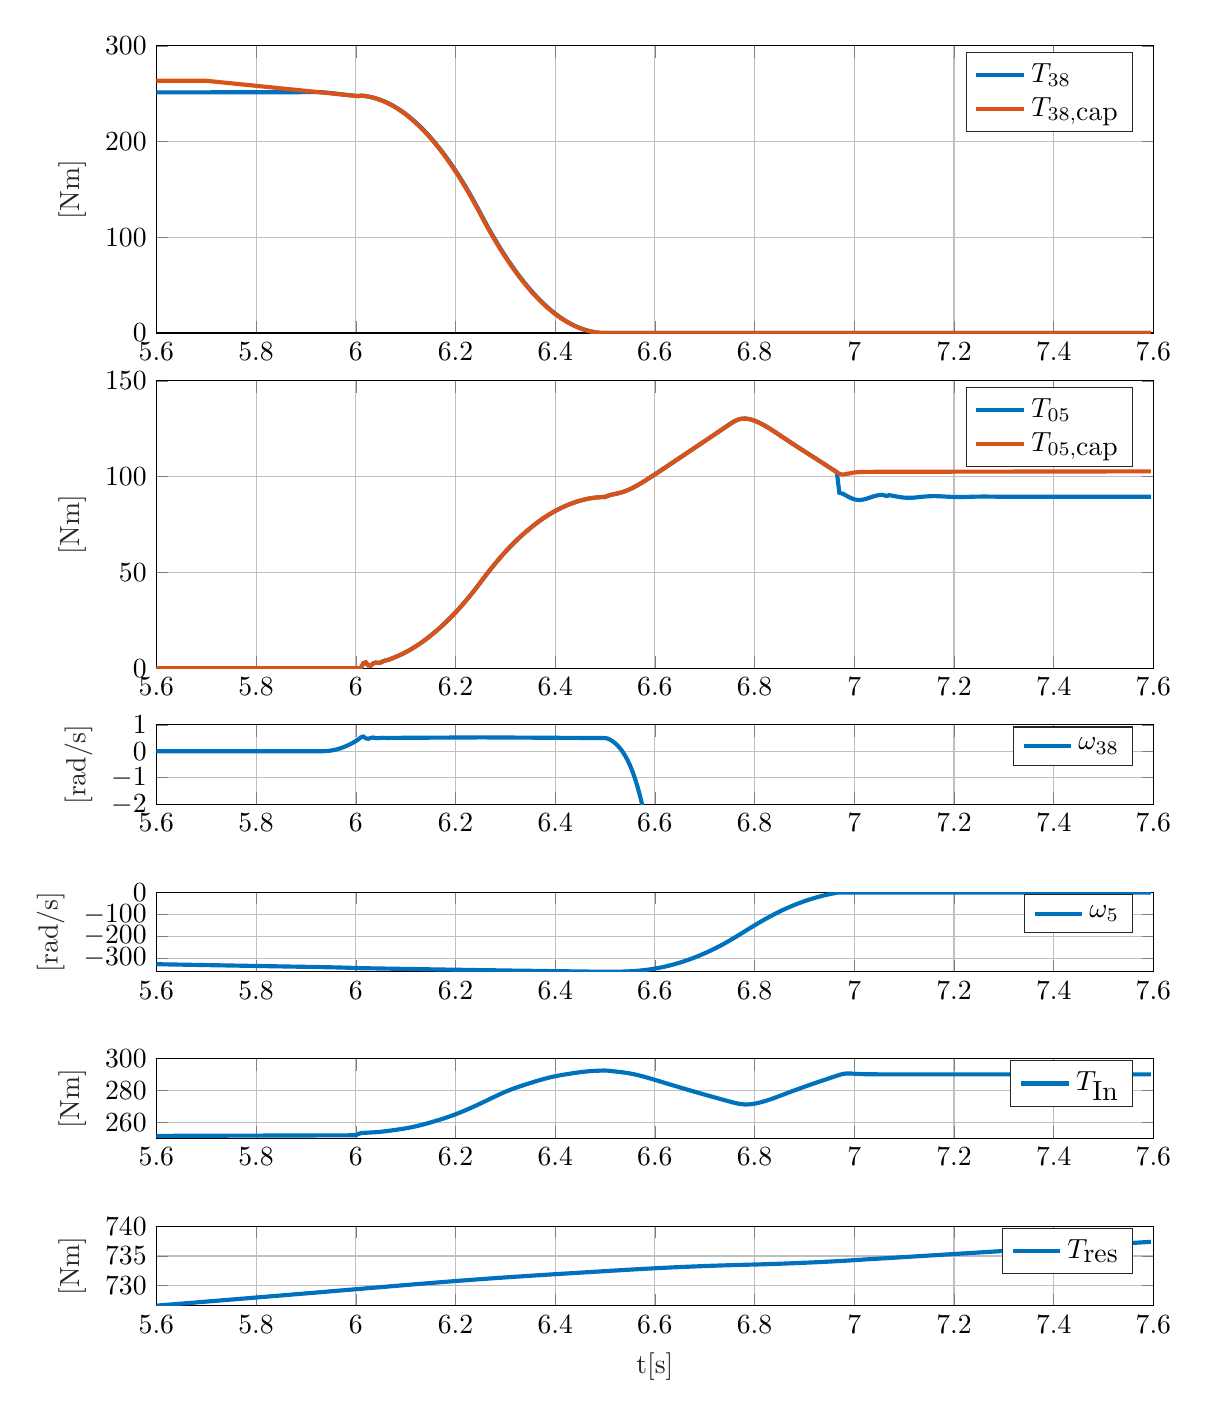
\begin{tikzpicture}

\begin{axis}[%
width=0.974\bwidth,
height=0.228\bheight,
at={(0\bwidth,0.772\bheight)},
scale only axis,
xmin=5.6,
xmax=7.6,
ymin=0,
ymax=300,
ylabel style={font=\color{white!15!black}},
ylabel={[Nm]},
axis background/.style={fill=white},
xmajorgrids,
ymajorgrids,
legend style={legend cell align=left, align=left, draw=white!15!black}
]
\addplot [color=mycolor1, line width=1.5pt]
  table[row sep=crcr]{%
5.6	251.324196937571\\
5.605	251.328551978443\\
5.61	251.33290902851\\
5.615	251.337268082622\\
5.62	251.341629146506\\
5.625	251.345992215012\\
5.63	251.350357293865\\
5.635	251.354724377912\\
5.64	251.359093472863\\
5.645	251.363464573576\\
5.65	251.367837685763\\
5.655	251.372212804266\\
5.66	251.376589934811\\
5.665	251.38096907223\\
5.67	251.385350222247\\
5.675	251.389733379721\\
5.68	251.394118550343\\
5.685	251.398505728966\\
5.69	251.402894921311\\
5.695	251.407286122193\\
5.7	251.411679337349\\
5.705	251.416062910737\\
5.71	251.420448640354\\
5.715	251.424839501019\\
5.72	251.429237905621\\
5.725	251.433642936822\\
5.73	251.43805188699\\
5.735	251.44246224286\\
5.74	251.446872226069\\
5.745	251.451281418915\\
5.75	251.455690607773\\
5.755	251.460100739669\\
5.76	251.464513084839\\
5.765	251.46892813986\\
5.77	251.473346189598\\
5.775	251.477766875941\\
5.78	251.482189783152\\
5.785	251.486614294736\\
5.79	251.491040084976\\
5.795	251.495466751604\\
5.8	251.499894367646\\
5.805	251.504322740688\\
5.81	251.508752176545\\
5.815	251.513182465594\\
5.82	251.517613896696\\
5.825	251.522046067573\\
5.83	251.526479142127\\
5.835	251.530912463331\\
5.84	251.535346091906\\
5.845	251.539779094508\\
5.85	251.54421148146\\
5.855	251.54864197792\\
5.86	251.553070556517\\
5.865	251.557495442153\\
5.87	251.561916518511\\
5.875	251.566331224249\\
5.88	251.570739232882\\
5.885	251.575136730134\\
5.89	251.579522967702\\
5.895	251.583892124382\\
5.9	251.587597690766\\
5.905	251.590655911881\\
5.91	251.593827451309\\
5.915	251.596912102685\\
5.92	251.599424356877\\
5.925	251.600626352389\\
5.93	251.546773355117\\
5.935	251.407267763264\\
5.94	251.200277998441\\
5.945	250.932248443384\\
5.95	250.617986110781\\
5.955	250.366732540807\\
5.96	250.046928719455\\
5.965	249.701923339615\\
5.97	249.375011920781\\
5.975	249.081076198104\\
5.98	248.796192446428\\
5.985	248.536640639005\\
5.99	248.320516814436\\
5.995	247.994706011143\\
6	247.738789781753\\
6.005	247.472310914202\\
6.01	247.861288594238\\
6.015	247.814492592787\\
6.02	247.493158181057\\
6.025	247.069550794376\\
6.03	246.546149568244\\
6.035	245.923855168622\\
6.04	245.202094174683\\
6.045	244.38086110607\\
6.05	243.460147884481\\
6.055	242.441088965125\\
6.06	241.322198550205\\
6.065	240.104022659404\\
6.07	238.786565847269\\
6.075	237.369828186045\\
6.08	235.853809679764\\
6.085	234.238510328337\\
6.09	232.523930131708\\
6.095	230.710069089877\\
6.1	228.796927202845\\
6.105	226.784504470611\\
6.11	224.672800893176\\
6.115	222.46181647054\\
6.12	220.151551202701\\
6.125	217.742005089662\\
6.13	215.233178131421\\
6.135	212.625070327978\\
6.14	209.917681679333\\
6.145	207.111012185487\\
6.15	204.20506184644\\
6.155	201.199830662191\\
6.16	198.095318632741\\
6.165	194.891525758089\\
6.17	191.588452038236\\
6.175	188.186097473181\\
6.18	184.684462062925\\
6.185	181.083545807466\\
6.19	177.383348706807\\
6.195	173.583870760946\\
6.2	169.685111969884\\
6.205	165.68707233362\\
6.21	161.589751852154\\
6.215	157.393150525487\\
6.22	153.097268353619\\
6.225	148.702105336548\\
6.23	144.207661474276\\
6.235	139.613936766803\\
6.24	134.920931214129\\
6.245	130.128644816253\\
6.25	125.237077573175\\
6.255	120.313741733389\\
6.26	115.475705221927\\
6.265	110.734669253283\\
6.27	106.095236064131\\
6.275	101.555121242504\\
6.28	97.1142889599688\\
6.285	92.772737596481\\
6.29	88.5304670810432\\
6.295	84.3874774107753\\
6.3	80.3458706637968\\
6.305	76.4015589709578\\
6.31	72.554050065605\\
6.315	68.8083413910594\\
6.32	65.1617452255521\\
6.325	61.6144367407819\\
6.33	58.1664134304146\\
6.335	54.8176704779849\\
6.34	51.568208412268\\
6.345	48.4180271943729\\
6.35	45.367126821173\\
6.355	42.4155072933716\\
6.36	39.5631686107236\\
6.365	36.8101107732855\\
6.37	34.1563337810477\\
6.375	31.6018376340116\\
6.38	29.1466223321769\\
6.385	26.7906878755438\\
6.39	24.5340342641117\\
6.395	22.3766614978816\\
6.4	20.318569576853\\
6.405	18.3597585010259\\
6.41	16.5002282704004\\
6.415	14.7399788849763\\
6.42	13.0790103447538\\
6.425	11.5173226497328\\
6.43	10.0549157999133\\
6.435	8.69178979529508\\
6.44	7.42794463587862\\
6.445	6.26338032166368\\
6.45	5.19809685265027\\
6.455	4.23209422883836\\
6.46	3.36537245022795\\
6.465	2.59793151681908\\
6.47	1.92977142861171\\
6.475	1.36089218560579\\
6.48	0.891293787801461\\
6.485	0.520976235198662\\
6.49	0.249939527797386\\
6.495	0.0781836655976118\\
6.5	0.00619796574077166\\
6.505	0.00377733821568384\\
6.51	0.00229111249439421\\
6.515	0.00139232751343445\\
6.52	0.000841144742537744\\
6.525	0.000510063906387214\\
6.53	0.000309602632626898\\
6.535	0.000187992886363182\\
6.54	0.000113721276075885\\
6.545	6.90721968009454e-05\\
6.55	4.18091389359936e-05\\
6.555	2.5338412082986e-05\\
6.56	1.53716289893082e-05\\
6.565	9.33263424607713e-06\\
6.57	5.67185547446161e-06\\
6.575	3.43959049472654e-06\\
6.58	2.08687647616106e-06\\
6.585	1.26586554508881e-06\\
6.59	7.68224899232963e-07\\
6.595	4.66583935628181e-07\\
6.6	2.82984645095339e-07\\
6.605	1.71655591560033e-07\\
6.61	1.04144245585539e-07\\
6.615	6.31765821085465e-08\\
6.62	3.83334318055354e-08\\
6.625	2.32627859157583e-08\\
6.63	1.41101534334219e-08\\
6.635	8.55908640195495e-09\\
6.64	5.1915622347523e-09\\
6.645	3.14917878796488e-09\\
6.65	1.9106359430392e-09\\
6.655	1.15902265733439e-09\\
6.66	7.03289725838386e-10\\
6.665	4.26584929568743e-10\\
6.67	2.58747717628157e-10\\
6.675	1.56948179008922e-10\\
6.68	9.52043017842951e-11\\
6.685	5.77466491799525e-11\\
6.69	3.50273315494778e-11\\
6.695	2.12475382682163e-11\\
6.7	1.28878545888591e-11\\
6.705	7.81735734425385e-12\\
6.71	4.74428236386198e-12\\
6.715	2.88162382163649e-12\\
6.72	1.74761807368688e-12\\
6.725	1.06002063464802e-12\\
6.73	6.42970472359502e-13\\
6.735	3.90134003928057e-13\\
6.74	2.36919721078311e-13\\
6.745	1.43755880224925e-13\\
6.75	8.72484366293792e-14\\
6.755	5.38733400988168e-14\\
6.76	3.26258553604051e-14\\
6.765	1.97225059241083e-14\\
6.77	1.1928961410259e-14\\
6.775	7.1918636208744e-15\\
6.78	4.33900587673293e-15\\
6.785	2.67376673220348e-15\\
6.79	1.67767734985315e-15\\
6.795	1.0547396760269e-15\\
6.8	6.63104728857857e-16\\
6.805	4.15877233405719e-16\\
6.81	2.60812638562521e-16\\
6.815	1.63555750292504e-16\\
6.82	1.02571661344003e-16\\
6.825	6.43227335922828e-17\\
6.83	4.03390867212266e-17\\
6.835	2.52966588788089e-17\\
6.84	1.58644395109732e-17\\
6.845	9.94859693740091e-18\\
6.85	6.23912094828646e-18\\
6.855	3.91255546817543e-18\\
6.86	2.45370346556681e-18\\
6.865	1.53871851356257e-18\\
6.87	9.64985411701006e-19\\
6.875	6.05142772604404e-19\\
6.88	3.79506675465632e-19\\
6.885	2.37988801725336e-19\\
6.89	1.49251289166214e-19\\
6.895	9.35955485395556e-20\\
6.9	5.8697115908297e-20\\
6.905	3.68089869897791e-20\\
6.91	2.30842322046219e-20\\
6.915	1.44761320848621e-20\\
6.92	9.07850016531353e-21\\
6.925	5.69313141371051e-21\\
6.93	3.57036632282255e-21\\
6.935	2.23897827843588e-21\\
6.94	1.40414335485163e-21\\
6.945	8.80538910314886e-22\\
6.95	5.52217442891262e-22\\
6.955	3.46295799314397e-22\\
6.96	2.17174480924411e-22\\
6.965	1.36190211719222e-22\\
6.97	8.51929069810571e-23\\
6.975	5.2359114364187e-23\\
6.98	3.18159293854717e-23\\
6.985	1.92960280456334e-23\\
6.99	1.19135905003199e-23\\
6.995	7.45889414681998e-24\\
7	4.51074744488547e-24\\
7.005	2.80583238375492e-24\\
7.01	1.73385087653402e-24\\
7.015	1.0715473388777e-24\\
7.02	6.55327343528648e-25\\
7.025	3.95671222636634e-25\\
7.03	2.39184287265332e-25\\
7.035	1.44360262345688e-25\\
7.04	8.69200087997607e-26\\
7.045	5.35053574122487e-26\\
7.05	3.28739529270217e-26\\
7.055	1.98810539083693e-26\\
7.06	1.19536131164434e-26\\
7.065	7.59808481066392e-27\\
7.07	4.67038506386851e-27\\
7.075	2.9593169737113e-27\\
7.08	1.86953444048416e-27\\
7.085	1.16725298659715e-27\\
7.09	7.34137088759513e-28\\
7.095	4.58071743161787e-28\\
7.1	2.76503170881651e-28\\
7.105	1.66400199194581e-28\\
7.11	1.00747166517643e-28\\
7.115	6.19690288372549e-29\\
7.12	3.94766872718641e-29\\
7.125	2.5036292991524e-29\\
7.13	1.57381097673192e-29\\
7.135	9.89584271611524e-30\\
7.14	6.14417104039723e-30\\
7.145	3.81521703463366e-30\\
7.15	2.34930155895606e-30\\
7.155	1.44624675456793e-30\\
7.16	9.08356944112569e-31\\
7.165	5.71926506980126e-31\\
7.17	3.53713187069668e-31\\
7.175	2.18349371705921e-31\\
7.18	1.35588340230326e-31\\
7.185	8.4267677823394e-32\\
7.19	5.24237729185508e-32\\
7.195	3.28955811650354e-32\\
7.2	2.06655490618733e-32\\
7.205	1.2792001057537e-32\\
7.21	7.75480585827525e-33\\
7.215	4.75209913410728e-33\\
7.22	2.95248378600685e-33\\
7.225	1.83452769735748e-33\\
7.23	1.1445807582281e-33\\
7.235	7.17907733942655e-34\\
7.24	4.4824046335537e-34\\
7.245	2.83325780056943e-34\\
7.25	1.80227228518813e-34\\
7.255	1.14180899676546e-34\\
7.26	7.1637020278124e-35\\
7.265	4.50872225217169e-35\\
7.27	2.80025129967748e-35\\
7.275	1.74032034906484e-35\\
7.28	1.08261993875402e-35\\
7.285	6.79195130209829e-36\\
7.29	4.26643019754435e-36\\
7.295	2.64869836435653e-36\\
7.3	1.64654696753994e-36\\
7.305	1.02507815997883e-36\\
7.31	6.45265988224715e-37\\
7.315	4.06704566967967e-37\\
7.32	2.52126962047223e-37\\
7.325	1.60480646703697e-37\\
7.33	1.01713474759999e-37\\
7.335	6.38636929057005e-38\\
7.34	4.01336669067741e-38\\
7.345	2.49143988238969e-38\\
7.35	1.54734190093586e-38\\
7.355	9.60929262683067e-39\\
7.36	5.97753194284246e-39\\
7.365	3.7307834160735e-39\\
7.37	2.30307946166181e-39\\
7.375	1.43751340482007e-39\\
7.38	9.01664047410467e-40\\
7.385	5.62510647854431e-40\\
7.39	3.57497972302587e-40\\
7.395	2.26334147466429e-40\\
7.4	1.41827778674988e-40\\
7.405	8.90531563365869e-41\\
7.41	5.5302164804545e-41\\
7.415	3.44430029394699e-41\\
7.42	2.16541119216108e-41\\
7.425	1.35804346660464e-41\\
7.43	8.51709965151481e-42\\
7.435	5.34095807161228e-42\\
7.44	3.34961840134291e-42\\
7.445	2.10050002890237e-42\\
7.45	1.31734295602463e-42\\
7.455	8.26087806050638e-43\\
7.46	5.18086616219751e-43\\
7.465	3.24885053037711e-43\\
7.47	2.04590705639284e-43\\
7.475	1.28361986349447e-43\\
7.48	8.05048049106732e-44\\
7.485	5.04835118138288e-44\\
7.49	3.16610808314576e-44\\
7.495	1.98542321302738e-44\\
7.5	1.24517174413782e-44\\
7.505	7.80830223116345e-45\\
7.51	4.89703013618507e-45\\
7.515	3.07086082850443e-45\\
7.52	1.93382114058301e-45\\
7.525	1.21329618603234e-45\\
7.53	7.6094313848874e-46\\
7.535	4.77177504674075e-46\\
7.54	2.99265146255151e-46\\
7.545	1.87665093111623e-46\\
7.55	1.17695446376532e-46\\
7.555	7.38052096721795e-47\\
7.56	4.62874419140202e-47\\
7.565	2.90262237054932e-47\\
7.57	1.82787590085324e-47\\
7.575	1.14682522209735e-47\\
7.58	7.21002223803319e-48\\
7.585	4.52178488311183e-48\\
7.59	2.83588069154112e-48\\
7.595	1.77834245099191e-48\\
};
\addlegendentry{$T_{38}$}

\addplot [color=mycolor2, line width=1.5pt]
  table[row sep=crcr]{%
5.6	263.484196394687\\
5.605	263.484196394687\\
5.61	263.484196394687\\
5.615	263.484196394687\\
5.62	263.484196394687\\
5.625	263.484196394687\\
5.63	263.484196394687\\
5.635	263.484196394687\\
5.64	263.484196394687\\
5.645	263.484196394687\\
5.65	263.484196394687\\
5.655	263.484196394687\\
5.66	263.484196394687\\
5.665	263.484196394687\\
5.67	263.484196394687\\
5.675	263.484196394687\\
5.68	263.484196394687\\
5.685	263.484196394687\\
5.69	263.484196394687\\
5.695	263.484196394687\\
5.7	263.484196394687\\
5.705	263.220712198292\\
5.71	262.957228001897\\
5.715	262.693743805503\\
5.72	262.430259609108\\
5.725	262.166775412713\\
5.73	261.903291216319\\
5.735	261.639807019924\\
5.74	261.376322823529\\
5.745	261.112838627135\\
5.75	260.84935443074\\
5.755	260.585870234345\\
5.76	260.322386037951\\
5.765	260.058901841556\\
5.77	259.795417645161\\
5.775	259.531933448767\\
5.78	259.268449252372\\
5.785	259.004965055977\\
5.79	258.741480859583\\
5.795	258.477996663188\\
5.8	258.214512466793\\
5.805	257.951028270399\\
5.81	257.687544074004\\
5.815	257.424059877609\\
5.82	257.160575681214\\
5.825	256.89709148482\\
5.83	256.633607288425\\
5.835	256.37012309203\\
5.84	256.106638895636\\
5.845	255.843154699241\\
5.85	255.579670502846\\
5.855	255.316186306452\\
5.86	255.052702110057\\
5.865	254.789217913662\\
5.87	254.525733717268\\
5.875	254.262249520873\\
5.88	253.998765324478\\
5.885	253.735281128084\\
5.89	253.471796931689\\
5.895	253.208312735294\\
5.9	252.944828538899\\
5.905	252.681344342505\\
5.91	252.41786014611\\
5.915	252.154375949715\\
5.92	251.890891753321\\
5.925	251.627407556926\\
5.93	251.363923360531\\
5.935	251.100439164137\\
5.94	250.836954967742\\
5.945	250.573470771347\\
5.95	250.309986574953\\
5.955	250.046502378558\\
5.96	249.783018182163\\
5.965	249.519533985769\\
5.97	249.256049789374\\
5.975	248.992565592979\\
5.98	248.729081396584\\
5.985	248.46559720019\\
5.99	248.202113003795\\
5.995	247.9386288074\\
6	247.675144611006\\
6.005	247.411660414611\\
6.01	248.003551313397\\
6.015	247.755349200395\\
6.02	247.407866242191\\
6.025	246.961102438785\\
6.03	246.415057790178\\
6.035	245.769732296369\\
6.04	245.025125957359\\
6.045	244.181238773147\\
6.05	243.238070743734\\
6.055	242.195621869119\\
6.06	241.053892149303\\
6.065	239.812881584285\\
6.07	238.472590174065\\
6.075	237.033017918645\\
6.08	235.494164818022\\
6.085	233.856030872198\\
6.09	232.118616081173\\
6.095	230.281920444946\\
6.1	228.345943963517\\
6.105	226.310686636887\\
6.11	224.176148465056\\
6.115	221.942329448023\\
6.12	219.609229585788\\
6.125	217.176848878352\\
6.13	214.645187325715\\
6.135	212.014244927876\\
6.14	209.284021684835\\
6.145	206.454517596593\\
6.15	203.525732663149\\
6.155	200.497666884504\\
6.16	197.370320260657\\
6.165	194.143692791609\\
6.17	190.817784477359\\
6.175	187.392595317908\\
6.18	183.868125313256\\
6.185	180.244374463401\\
6.19	176.521342768345\\
6.195	172.699030228088\\
6.2	168.777436842629\\
6.205	164.756562611969\\
6.21	160.636407536107\\
6.215	156.416971615044\\
6.22	152.098254848779\\
6.225	147.680257237312\\
6.23	143.162978780644\\
6.235	138.546419478774\\
6.24	133.830579331703\\
6.245	129.015458339431\\
6.25	124.101056501957\\
6.255	119.18665466448\\
6.26	114.371533672206\\
6.265	109.655693525131\\
6.27	105.03913422326\\
6.275	100.52185576659\\
6.28	96.103858155121\\
6.285	91.7851413888538\\
6.29	87.5657054677882\\
6.295	83.4455503919241\\
6.3	79.4246761612615\\
6.305	75.5030827758004\\
6.31	71.6807702355402\\
6.315	67.9577385404821\\
6.32	64.3339876906256\\
6.325	60.8095176859706\\
6.33	57.3843285265171\\
6.335	54.0584202122652\\
6.34	50.8317927432147\\
6.345	47.7044461193658\\
6.35	44.6763803407178\\
6.355	41.7475954072719\\
6.36	38.9180913190275\\
6.365	36.1878680759847\\
6.37	33.5569256781433\\
6.375	31.0252641255035\\
6.38	28.5928834180652\\
6.385	26.2597835558284\\
6.39	24.0259645387927\\
6.395	21.8914263669589\\
6.4	19.8561690403267\\
6.405	17.9201925588959\\
6.41	16.0834969226667\\
6.415	14.3460821316391\\
6.42	12.7079481858129\\
6.425	11.1690950851882\\
6.43	9.72952282976506\\
6.435	8.38923141954318\\
6.44	7.14822085452309\\
6.445	6.00649113470448\\
6.45	4.96404226008743\\
6.455	4.02087423067186\\
6.46	3.1769870464578\\
6.465	2.43238070744528\\
6.47	1.78705521363426\\
6.475	1.2410105650247\\
6.48	0.794246761616723\\
6.485	0.446763803410259\\
6.49	0.198561690405331\\
6.495	0.0496404226019115\\
6.5	0\\
6.505	0\\
6.51	0\\
6.515	0\\
6.52	0\\
6.525	0\\
6.53	0\\
6.535	0\\
6.54	0\\
6.545	0\\
6.55	0\\
6.555	0\\
6.56	0\\
6.565	0\\
6.57	0\\
6.575	0\\
6.58	0\\
6.585	0\\
6.59	0\\
6.595	0\\
6.6	0\\
6.605	0\\
6.61	0\\
6.615	0\\
6.62	0\\
6.625	0\\
6.63	0\\
6.635	0\\
6.64	0\\
6.645	0\\
6.65	0\\
6.655	0\\
6.66	0\\
6.665	0\\
6.67	0\\
6.675	0\\
6.68	0\\
6.685	0\\
6.69	0\\
6.695	0\\
6.7	0\\
6.705	0\\
6.71	0\\
6.715	0\\
6.72	0\\
6.725	0\\
6.73	0\\
6.735	0\\
6.74	0\\
6.745	0\\
6.75	0\\
6.755	0\\
6.76	0\\
6.765	0\\
6.77	0\\
6.775	0\\
6.78	0\\
6.785	0\\
6.79	0\\
6.795	0\\
6.8	0\\
6.805	0\\
6.81	0\\
6.815	0\\
6.82	0\\
6.825	0\\
6.83	0\\
6.835	0\\
6.84	0\\
6.845	0\\
6.85	0\\
6.855	0\\
6.86	0\\
6.865	0\\
6.87	0\\
6.875	0\\
6.88	0\\
6.885	0\\
6.89	0\\
6.895	0\\
6.9	0\\
6.905	0\\
6.91	0\\
6.915	0\\
6.92	0\\
6.925	0\\
6.93	0\\
6.935	0\\
6.94	0\\
6.945	0\\
6.95	0\\
6.955	0\\
6.96	0\\
6.965	0\\
6.97	0\\
6.975	0\\
6.98	0\\
6.985	0\\
6.99	0\\
6.995	0\\
7	0\\
7.005	0\\
7.01	0\\
7.015	0\\
7.02	0\\
7.025	0\\
7.03	0\\
7.035	0\\
7.04	0\\
7.045	0\\
7.05	0\\
7.055	0\\
7.06	0\\
7.065	0\\
7.07	0\\
7.075	0\\
7.08	0\\
7.085	0\\
7.09	0\\
7.095	0\\
7.1	0\\
7.105	0\\
7.11	0\\
7.115	0\\
7.12	0\\
7.125	0\\
7.13	0\\
7.135	0\\
7.14	0\\
7.145	0\\
7.15	0\\
7.155	0\\
7.16	0\\
7.165	0\\
7.17	0\\
7.175	0\\
7.18	0\\
7.185	0\\
7.19	0\\
7.195	0\\
7.2	0\\
7.205	0\\
7.21	0\\
7.215	0\\
7.22	0\\
7.225	0\\
7.23	0\\
7.235	0\\
7.24	0\\
7.245	0\\
7.25	0\\
7.255	0\\
7.26	0\\
7.265	0\\
7.27	0\\
7.275	0\\
7.28	0\\
7.285	0\\
7.29	0\\
7.295	0\\
7.3	0\\
7.305	0\\
7.31	0\\
7.315	0\\
7.32	0\\
7.325	0\\
7.33	0\\
7.335	0\\
7.34	0\\
7.345	0\\
7.35	0\\
7.355	0\\
7.36	0\\
7.365	0\\
7.37	0\\
7.375	0\\
7.38	0\\
7.385	0\\
7.39	0\\
7.395	0\\
7.4	0\\
7.405	0\\
7.41	0\\
7.415	0\\
7.42	0\\
7.425	0\\
7.43	0\\
7.435	0\\
7.44	0\\
7.445	0\\
7.45	0\\
7.455	0\\
7.46	0\\
7.465	0\\
7.47	0\\
7.475	0\\
7.48	0\\
7.485	0\\
7.49	0\\
7.495	0\\
7.5	0\\
7.505	0\\
7.51	0\\
7.515	0\\
7.52	0\\
7.525	0\\
7.53	0\\
7.535	0\\
7.54	0\\
7.545	0\\
7.55	0\\
7.555	0\\
7.56	0\\
7.565	0\\
7.57	0\\
7.575	0\\
7.58	0\\
7.585	0\\
7.59	0\\
7.595	0\\
};
\addlegendentry{$T_{38,\textrm{cap}}$}

\end{axis}

\begin{axis}[%
width=0.974\bwidth,
height=0.228\bheight,
at={(0\bwidth,0.506\bheight)},
scale only axis,
xmin=5.6,
xmax=7.6,
ymin=-0,
ymax=150,
ylabel style={font=\color{white!15!black}},
ylabel={[Nm]},
axis background/.style={fill=white},
xmajorgrids,
ymajorgrids,
legend style={legend cell align=left, align=left, draw=white!15!black}
]
\addplot [color=mycolor1, line width=1.5pt]
  table[row sep=crcr]{%
5.6	-0\\
5.605	-0\\
5.61	-0\\
5.615	-0\\
5.62	-0\\
5.625	-0\\
5.63	-0\\
5.635	-0\\
5.64	-0\\
5.645	-0\\
5.65	-0\\
5.655	-0\\
5.66	-0\\
5.665	-0\\
5.67	-0\\
5.675	-0\\
5.68	-0\\
5.685	-0\\
5.69	-0\\
5.695	-0\\
5.7	-0\\
5.705	-0\\
5.71	-0\\
5.715	-0\\
5.72	-0\\
5.725	-0\\
5.73	-0\\
5.735	-0\\
5.74	-0\\
5.745	-0\\
5.75	-0\\
5.755	-0\\
5.76	-0\\
5.765	-0\\
5.77	-0\\
5.775	-0\\
5.78	-0\\
5.785	-0\\
5.79	-0\\
5.795	-0\\
5.8	-0\\
5.805	-0\\
5.81	-0\\
5.815	-0\\
5.82	-0\\
5.825	-0\\
5.83	-0\\
5.835	-0\\
5.84	-0\\
5.845	-0\\
5.85	-0\\
5.855	-0\\
5.86	-0\\
5.865	-0\\
5.87	-0\\
5.875	-0\\
5.88	-0\\
5.885	-0\\
5.89	-0\\
5.895	-0\\
5.9	-0\\
5.905	-0\\
5.91	-0\\
5.915	-0\\
5.92	-0\\
5.925	-0\\
5.93	-0\\
5.935	-0\\
5.94	-0\\
5.945	-0\\
5.95	-0\\
5.955	-0\\
5.96	-0\\
5.965	-0\\
5.97	-0\\
5.975	-0\\
5.98	-0\\
5.985	-0\\
5.99	-0\\
5.995	-0\\
6	-0\\
6.005	-0\\
6.01	-0\\
6.015	2.590920767312\\
6.02	3.05538537596246\\
6.025	1.53832413661992\\
6.03	1.31339415784597\\
6.035	2.57066398730906\\
6.04	2.94507157469557\\
6.045	2.75275367226818\\
6.05	2.97973896261529\\
6.055	3.60963164989579\\
6.06	4.05029788541533\\
6.065	4.34743857096528\\
6.07	4.79094270680897\\
6.075	5.36321668939836\\
6.08	5.90578383393659\\
6.085	6.43389937709218\\
6.09	7.01781368947509\\
6.095	7.66863455843472\\
6.1	8.34053271228045\\
6.105	9.02968565658785\\
6.11	9.75857054739445\\
6.115	10.5363556590879\\
6.12	11.3498496799844\\
6.125	12.1942277157253\\
6.13	13.0756307124866\\
6.135	13.9973822866917\\
6.14	14.9556698377447\\
6.145	15.9469062358761\\
6.15	16.9716422061934\\
6.155	18.0312632700317\\
6.16	19.1247166588686\\
6.165	20.2505165761907\\
6.17	21.4091290728937\\
6.175	22.6018729539312\\
6.18	23.8290230638769\\
6.185	25.0907410700136\\
6.19	26.3878775546037\\
6.195	27.7213256503196\\
6.2	29.0913219449715\\
6.205	30.4978507575902\\
6.21	31.9409230169137\\
6.215	33.4203438722138\\
6.22	34.9356005780749\\
6.225	36.4860897047462\\
6.23	38.0712824646645\\
6.235	39.6907303931982\\
6.24	41.344056844046\\
6.245	43.0310717339226\\
6.25	44.7518188131861\\
6.255	46.4964364111416\\
6.26	48.2180525945561\\
6.265	49.8987476070888\\
6.27	51.5375385742653\\
6.275	53.1520313778476\\
6.28	54.7428171289908\\
6.285	56.2971158672275\\
6.29	57.8128466101952\\
6.295	59.2941094164566\\
6.3	60.7392764570452\\
6.305	62.1450288902284\\
6.31	63.5147584046801\\
6.315	64.8414899642169\\
6.32	66.1285429177347\\
6.325	67.3801828471616\\
6.33	68.5965801641768\\
6.335	69.7768438390705\\
6.34	70.922679558272\\
6.345	72.037007562478\\
6.35	73.120413163014\\
6.355	74.1716697697835\\
6.36	75.1904657253833\\
6.365	76.1770346208059\\
6.37	77.1301330667036\\
6.375	78.0479013272521\\
6.38	78.9292255040116\\
6.385	79.7736622014681\\
6.39	80.5804755406101\\
6.395	81.3491679622698\\
6.4	82.0800346764271\\
6.405	82.7738873786196\\
6.41	83.4315358411052\\
6.415	84.0538309099942\\
6.42	84.6418044613339\\
6.425	85.1964107135072\\
6.43	85.7181546659497\\
6.435	86.207208334081\\
6.44	86.6634828397309\\
6.445	87.0865831565525\\
6.45	87.4758001773396\\
6.455	87.8302895038469\\
6.46	88.1492416660879\\
6.465	88.4319556412199\\
6.47	88.6779045172028\\
6.475	88.8868302750928\\
6.48	89.0587864840147\\
6.485	89.1941002488993\\
6.49	89.2932980974518\\
6.495	89.3570338908719\\
6.5	89.3859986683963\\
6.505	89.9870475145159\\
6.51	90.3986145664207\\
6.515	90.6988246715875\\
6.52	90.9649801326458\\
6.525	91.2427344826775\\
6.53	91.5631850656054\\
6.535	91.9424062391424\\
6.54	92.3868365489822\\
6.545	92.8974482186568\\
6.55	93.4681159804892\\
6.555	94.094727205531\\
6.56	94.7709175048992\\
6.565	95.4892431186686\\
6.57	96.2425813416954\\
6.575	97.0243587513044\\
6.58	97.8287938669785\\
6.585	98.6509085369639\\
6.59	99.4865523320946\\
6.595	100.332342604943\\
6.6	101.185577092396\\
6.605	102.044189314342\\
6.61	102.906616681497\\
6.615	103.771708844943\\
6.62	104.638645507351\\
6.625	105.506851647521\\
6.63	106.375931414801\\
6.635	107.245616806572\\
6.64	108.115724550577\\
6.645	108.986130539444\\
6.65	109.856753291624\\
6.655	110.72754615558\\
6.66	111.598494888999\\
6.665	112.469616289318\\
6.67	113.34095926129\\
6.675	114.212601326339\\
6.68	115.08464337387\\
6.685	115.95720092634\\
6.69	116.830393039908\\
6.695	117.704329813001\\
6.7	118.579100311776\\
6.705	119.454762781865\\
6.71	120.331337783803\\
6.715	121.208807186144\\
6.72	122.08711631842\\
6.725	122.966179944773\\
6.73	123.845894182364\\
6.735	124.726148504779\\
6.74	125.60683801578\\
6.745	126.487874572352\\
6.75	127.369195950834\\
6.755	128.226633373231\\
6.76	128.992550134274\\
6.765	129.606556587103\\
6.77	130.041857666855\\
6.775	130.292685636092\\
6.78	130.367035435166\\
6.785	130.269891480503\\
6.79	130.030706912973\\
6.795	129.678797689936\\
6.8	129.230279662187\\
6.805	128.69966370634\\
6.81	128.09817080977\\
6.815	127.436474977065\\
6.82	126.723627769675\\
6.825	125.967919535745\\
6.83	125.176670173171\\
6.835	124.356984592847\\
6.84	123.515340838756\\
6.845	122.658056655293\\
6.85	121.790749958544\\
6.855	120.918575521994\\
6.86	120.045727985701\\
6.865	119.175607232311\\
6.87	118.310493006602\\
6.875	117.451778849032\\
6.88	116.599837069429\\
6.885	115.754374343556\\
6.89	114.914406078739\\
6.895	114.078698822457\\
6.9	113.245735393824\\
6.905	112.414166217517\\
6.91	111.582675422001\\
6.915	110.750373379183\\
6.92	109.916537929217\\
6.925	109.080922408207\\
6.93	108.243405029359\\
6.935	107.404230182717\\
6.94	106.563626647753\\
6.945	105.72202344994\\
6.95	104.879690326273\\
6.955	104.036967650201\\
6.96	103.193954077101\\
6.965	102.350771332833\\
6.97	91.5754655690193\\
6.975	91.2653365326729\\
6.98	90.6581435571034\\
6.985	89.9540856688238\\
6.99	89.2525731484024\\
6.995	88.6513191009155\\
7	88.1768584994799\\
7.005	87.9078534155576\\
7.01	87.8291369956371\\
7.015	87.9336452318532\\
7.02	88.1829366388115\\
7.025	88.5394320409388\\
7.03	88.9644732550863\\
7.035	89.4069803425172\\
7.04	89.822335243476\\
7.045	90.1625286635622\\
7.05	90.4197827740645\\
7.055	90.5611255284133\\
7.06	90.2637699980088\\
7.065	89.8815222914729\\
7.07	90.3557898946395\\
7.075	90.1346946489379\\
7.08	89.8882001379367\\
7.085	89.6393844991151\\
7.09	89.4121733804858\\
7.095	89.2229980821237\\
7.1	89.0783709843197\\
7.105	88.9917580820296\\
7.11	88.9659071487479\\
7.115	89.0047112230629\\
7.12	89.0827352114132\\
7.125	89.2039348906615\\
7.13	89.3366038195007\\
7.135	89.4698298806321\\
7.14	89.5940606484423\\
7.145	89.6994666505015\\
7.15	89.7783663588891\\
7.155	89.8256570109023\\
7.16	89.8378672142597\\
7.165	89.8213000240137\\
7.17	89.7803775447598\\
7.175	89.7218292685634\\
7.18	89.6521484723583\\
7.185	89.5796419599635\\
7.19	89.5115837712062\\
7.195	89.4545295407582\\
7.2	89.4123487633379\\
7.205	89.3855942859092\\
7.21	89.3747140769566\\
7.215	89.3811769707591\\
7.22	89.4025481732952\\
7.225	89.4339793892694\\
7.23	89.4714976525622\\
7.235	89.5106855214704\\
7.24	89.5473807664061\\
7.245	89.5781742270756\\
7.25	89.6009074381548\\
7.255	89.6147234314362\\
7.26	89.6201542370854\\
7.265	89.6171228012876\\
7.27	89.6070130426275\\
7.275	89.5914834616039\\
7.28	89.5725056941145\\
7.285	89.5523529536039\\
7.29	89.5331720873332\\
7.295	89.5163429271244\\
7.3	89.5032903595332\\
7.305	89.4948380119248\\
7.31	89.4914462184035\\
7.315	89.4914423718254\\
7.32	89.4982183777922\\
7.325	89.5036843920738\\
7.33	89.5145570075553\\
7.335	89.5255091553868\\
7.34	89.5350748760111\\
7.345	89.5438022675349\\
7.35	89.5508017009974\\
7.355	89.555437028559\\
7.36	89.5576022903967\\
7.365	89.5573690581979\\
7.37	89.5550714615303\\
7.375	89.5510598233359\\
7.38	89.5459746318591\\
7.385	89.5404441102271\\
7.39	89.5350868153758\\
7.395	89.5303725912169\\
7.4	89.5265523272887\\
7.405	89.52393638257\\
7.41	89.522523749737\\
7.415	89.5223761636492\\
7.42	89.523485717833\\
7.425	89.5252781115789\\
7.43	89.5277221913987\\
7.435	89.5304507681166\\
7.44	89.5331442721331\\
7.445	89.5355645397372\\
7.45	89.5375136091042\\
7.455	89.5388606998308\\
7.46	89.539547987703\\
7.465	89.5395657068721\\
7.47	89.5390484616158\\
7.475	89.5380476914895\\
7.48	89.5367272349091\\
7.485	89.5352432714634\\
7.49	89.5337477804103\\
7.495	89.5323752514196\\
7.5	89.5312322847529\\
7.505	89.5303908080535\\
7.51	89.5298861712522\\
7.515	89.5297176636351\\
7.52	89.5299102738033\\
7.525	89.5302656737237\\
7.53	89.5307934017634\\
7.535	89.5314588128177\\
7.54	89.5321328803439\\
7.545	89.5327485107212\\
7.55	89.5332555123323\\
7.555	89.5336125812156\\
7.56	89.5337979837109\\
7.565	89.5338047024008\\
7.57	89.5336625796003\\
7.575	89.5333834535015\\
7.58	89.5330075463159\\
7.585	89.5325770397353\\
7.59	89.5321318556223\\
7.595	89.5317090698277\\
};
\addlegendentry{$T_{05}$}

\addplot [color=mycolor2, line width=1.5pt]
  table[row sep=crcr]{%
5.6	-0\\
5.605	-0\\
5.61	-0\\
5.615	-0\\
5.62	-0\\
5.625	-0\\
5.63	-0\\
5.635	-0\\
5.64	-0\\
5.645	-0\\
5.65	-0\\
5.655	-0\\
5.66	-0\\
5.665	-0\\
5.67	-0\\
5.675	-0\\
5.68	-0\\
5.685	-0\\
5.69	-0\\
5.695	-0\\
5.7	-0\\
5.705	-0\\
5.71	-0\\
5.715	-0\\
5.72	-0\\
5.725	-0\\
5.73	-0\\
5.735	-0\\
5.74	-0\\
5.745	-0\\
5.75	-0\\
5.755	-0\\
5.76	-0\\
5.765	-0\\
5.77	-0\\
5.775	-0\\
5.78	-0\\
5.785	-0\\
5.79	-0\\
5.795	-0\\
5.8	-0\\
5.805	-0\\
5.81	-0\\
5.815	-0\\
5.82	-0\\
5.825	-0\\
5.83	-0\\
5.835	-0\\
5.84	-0\\
5.845	-0\\
5.85	-0\\
5.855	-0\\
5.86	-0\\
5.865	-0\\
5.87	-0\\
5.875	-0\\
5.88	-0\\
5.885	-0\\
5.89	-0\\
5.895	-0\\
5.9	-0\\
5.905	-0\\
5.91	-0\\
5.915	-0\\
5.92	-0\\
5.925	-0\\
5.93	-0\\
5.935	-0\\
5.94	-0\\
5.945	-0\\
5.95	-0\\
5.955	-0\\
5.96	-0\\
5.965	-0\\
5.97	-0\\
5.975	-0\\
5.98	-0\\
5.985	-0\\
5.99	-0\\
5.995	-0\\
6	-0\\
6.005	-0\\
6.01	-0\\
6.015	2.23127228447488\\
6.02	3.03563758185093\\
6.025	1.45929083947103\\
6.03	1.24983114276596\\
6.035	2.47511004907197\\
6.04	2.94640888593676\\
6.045	2.74262304828911\\
6.05	2.95817493984239\\
6.055	3.57789841744123\\
6.06	4.04182730065456\\
6.065	4.34250386348257\\
6.07	4.77513739368296\\
6.075	5.34490598053442\\
6.08	5.89295427837295\\
6.085	6.42246128548053\\
6.09	7.00379623555403\\
6.095	7.65337175651864\\
6.1	8.32673639811236\\
6.105	9.01671798573207\\
6.11	9.74507002746321\\
6.115	10.5224952843225\\
6.12	11.336536719872\\
6.125	12.1814972053767\\
6.13	13.0631627229832\\
6.135	13.9851829626748\\
6.14	14.9440762713592\\
6.145	15.9360754335611\\
6.15	16.9615310428413\\
6.155	18.0218711525982\\
6.16	19.1161560186987\\
6.165	20.2428564353415\\
6.17	21.4023461388718\\
6.175	22.5959542699532\\
6.18	23.8239961231602\\
6.185	25.0866201260764\\
6.19	26.3846532810792\\
6.195	27.7190040290192\\
6.2	29.0899309093295\\
6.205	30.4974199354678\\
6.21	31.9414805128725\\
6.215	33.4219255613521\\
6.22	34.9382478979644\\
6.225	36.4898410972784\\
6.23	38.0761701227951\\
6.235	39.6967824517627\\
6.24	41.3512962817382\\
6.245	43.0395141670295\\
6.25	44.761473471146\\
6.255	46.5077831602961\\
6.26	48.2319628505318\\
6.265	49.9153350467953\\
6.27	51.5562983744503\\
6.275	53.1724958365492\\
6.28	54.7649382700448\\
6.285	56.320847713679\\
6.29	57.8379846901036\\
6.295	59.3204412036571\\
6.3	60.7666660231817\\
6.305	62.1733360722518\\
6.31	63.5438447732294\\
6.315	64.8711997112917\\
6.32	66.1587410049369\\
6.325	67.4107624578419\\
6.33	68.6274331461875\\
6.335	69.8078636451217\\
6.34	70.953794773819\\
6.345	72.0681603661868\\
6.35	73.1515266645481\\
6.355	74.2026585939548\\
6.36	75.2212631352369\\
6.365	76.2075721931431\\
6.37	77.1603194055995\\
6.375	78.0776385958003\\
6.38	78.9584332955382\\
6.385	79.802260941724\\
6.39	80.608382132692\\
6.395	81.3763091499164\\
6.4	82.106358989701\\
6.405	82.7993552109494\\
6.41	83.4561100920204\\
6.415	84.0774824898939\\
6.42	84.6645164732162\\
6.425	85.2181598518157\\
6.43	85.738909625875\\
6.435	86.226929744059\\
6.44	86.6821235931818\\
6.445	87.1040844125255\\
6.45	87.4920919163786\\
6.455	87.845296662029\\
6.46	88.1628890218861\\
6.465	88.4441702355675\\
6.47	88.6886193814804\\
6.475	88.8959891592134\\
6.48	89.0663460094956\\
6.485	89.2000287802644\\
6.49	89.2975735088285\\
6.495	89.3596409918641\\
6.5	89.386924758005\\
6.505	90.0088540836117\\
6.51	90.4145139116018\\
6.515	90.7114864184326\\
6.52	90.9768914989763\\
6.525	91.2556296111595\\
6.53	91.5780055597617\\
6.535	91.959537230123\\
6.54	92.4063087612254\\
6.545	92.9190816899122\\
6.55	93.4916779763713\\
6.555	94.1199765828117\\
6.56	94.7975823945926\\
6.565	95.5170768149966\\
6.57	96.2713695468504\\
6.575	97.0539196781284\\
6.58	97.8589764637861\\
6.585	98.6815889102185\\
6.59	99.5176303347744\\
6.595	100.363738487503\\
6.6	101.217228476945\\
6.605	102.076048244136\\
6.61	102.938647010086\\
6.615	103.803883875669\\
6.62	104.670945858785\\
6.625	105.539263429661\\
6.63	106.408444712132\\
6.635	107.278224467591\\
6.64	108.14842133024\\
6.645	109.018912527111\\
6.65	109.889617591082\\
6.655	110.760490758337\\
6.66	111.631518649465\\
6.665	112.502718938689\\
6.67	113.374141416819\\
6.675	114.245864411834\\
6.68	115.117989458607\\
6.685	115.990632470328\\
6.69	116.863912570489\\
6.695	117.73793957214\\
6.7	118.612801916283\\
6.705	119.488556958702\\
6.71	120.365224198292\\
6.715	121.242784416121\\
6.72	122.121181906167\\
6.725	123.000330672507\\
6.73	123.880126347612\\
6.735	124.760458288537\\
6.74	125.641221828798\\
6.745	126.522329372189\\
6.75	127.403719485533\\
6.755	128.26004255767\\
6.76	129.022379813395\\
6.765	129.630756673226\\
6.77	130.059020067459\\
6.775	130.301990419786\\
6.78	130.368181729591\\
6.785	130.263462382881\\
6.79	130.017903048785\\
6.795	129.660509372475\\
6.8	129.207261194697\\
6.805	128.672580361691\\
6.81	128.067621787117\\
6.815	127.402980394748\\
6.82	126.687637610409\\
6.825	125.929838843339\\
6.83	125.136866782548\\
6.835	124.315807493448\\
6.84	123.473116137768\\
6.845	122.615093857732\\
6.85	121.747329174896\\
6.855	120.874946186028\\
6.86	120.00209543357\\
6.865	119.132131711061\\
6.87	118.267282390669\\
6.875	117.408893539514\\
6.88	116.557290679902\\
6.885	115.712145301086\\
6.89	114.872443325141\\
6.895	114.036936945231\\
6.9	113.204100287882\\
6.905	112.372589290641\\
6.91	111.541095134329\\
6.915	110.708745386902\\
6.92	109.874831143614\\
6.925	109.039124460361\\
6.93	108.201514148843\\
6.935	107.362257512586\\
6.94	106.521586588384\\
6.945	105.679935214076\\
6.95	104.837569177393\\
6.955	103.994827635572\\
6.96	103.151801371001\\
6.965	102.308608920376\\
6.97	101.492713898566\\
6.975	101.165774387776\\
6.98	101.198331499003\\
6.985	101.418631914693\\
6.99	101.702937878314\\
6.995	101.970710309272\\
7	102.186819304515\\
7.005	102.32059550984\\
7.01	102.404748714796\\
7.015	102.456847304751\\
7.02	102.489811237289\\
7.025	102.510735996884\\
7.03	102.523893629088\\
7.035	102.532602480299\\
7.04	102.538792048967\\
7.045	102.543524324192\\
7.05	102.547608799327\\
7.055	102.551352311578\\
7.06	102.554839114643\\
7.065	102.558175812858\\
7.07	102.561437232122\\
7.075	102.564478707302\\
7.08	102.56729341306\\
7.085	102.569885175576\\
7.09	102.572226317979\\
7.095	102.574349993406\\
7.1	102.576298710915\\
7.105	102.578082630819\\
7.11	102.57974730334\\
7.115	102.58135609883\\
7.12	102.582970437843\\
7.125	102.584647992897\\
7.13	102.586410092278\\
7.135	102.588280802857\\
7.14	102.590258304509\\
7.145	102.592350613638\\
7.15	102.59454206464\\
7.155	102.596817156545\\
7.16	102.599152896952\\
7.165	102.601513963455\\
7.17	102.603878278956\\
7.175	102.606221480848\\
7.18	102.608521559167\\
7.185	102.61076554095\\
7.19	102.61294668592\\
7.195	102.615063529132\\
7.2	102.61712532403\\
7.205	102.619145823397\\
7.21	102.621135992973\\
7.215	102.623106874787\\
7.22	102.625076842698\\
7.225	102.627059709282\\
7.23	102.6290663271\\
7.235	102.631104596544\\
7.24	102.633175719329\\
7.245	102.635281946012\\
7.25	102.637418328451\\
7.255	102.639577287794\\
7.26	102.641751958076\\
7.265	102.643935767846\\
7.27	102.646122058612\\
7.275	102.648303908713\\
7.28	102.650475270467\\
7.285	102.652631429934\\
7.29	102.654770688957\\
7.295	102.656894213806\\
7.3	102.659002091032\\
7.305	102.661097027009\\
7.31	102.663182562067\\
7.315	102.665263439445\\
7.32	102.667344850108\\
7.325	102.6694277633\\
7.33	102.671517537717\\
7.335	102.673615811459\\
7.34	102.675722808102\\
7.345	102.677838086939\\
7.35	102.679962040352\\
7.355	102.682093302817\\
7.36	102.684230164017\\
7.365	102.686370501159\\
7.37	102.688512402873\\
7.375	102.69065380187\\
7.38	102.692792837582\\
7.385	102.694928513778\\
7.39	102.69705964301\\
7.395	102.699186553003\\
7.4	102.701309811675\\
7.405	102.703429744473\\
7.41	102.705547399019\\
7.415	102.707663651869\\
7.42	102.709779802126\\
7.425	102.711896772068\\
7.43	102.714015419538\\
7.435	102.716136378047\\
7.44	102.718259989183\\
7.445	102.720386355795\\
7.45	102.722515356043\\
7.455	102.724646671051\\
7.46	102.726779846715\\
7.465	102.728914345608\\
7.47	102.731049662122\\
7.475	102.733185228357\\
7.48	102.735320603752\\
7.485	102.737455441912\\
7.49	102.739589529066\\
7.495	102.7417227848\\
7.5	102.743855254423\\
7.505	102.745987087737\\
7.51	102.74811851238\\
7.515	102.750249802752\\
7.52	102.75238127166\\
7.525	102.754513197498\\
7.53	102.756645759549\\
7.535	102.7587791805\\
7.54	102.760913571772\\
7.545	102.763048971243\\
7.55	102.76518536514\\
7.555	102.767322683881\\
7.56	102.769460817996\\
7.565	102.771599630796\\
7.57	102.773738994222\\
7.575	102.775878747577\\
7.58	102.778018775445\\
7.585	102.78015897174\\
7.59	102.782299275134\\
7.595	102.784439653554\\
};
\addlegendentry{$T_{05,\textrm{cap}}$}

\end{axis}

\begin{axis}[%
width=0.974\bwidth,
height=0.063\bheight,
at={(0\bwidth,0.398\bheight)},
scale only axis,
xmin=5.6,
xmax=7.6,
ymin=-2,
ymax=1,
ylabel style={font=\color{white!15!black}},
ylabel={[rad/s]},
axis background/.style={fill=white},
xmajorgrids,
ymajorgrids,
legend style={legend cell align=left, align=left, draw=white!15!black}
]
\addplot [color=mycolor1, line width=1.5pt]
  table[row sep=crcr]{%
5.6	8.64051042981373e-06\\
5.605	8.64912090037251e-06\\
5.61	8.65774325120583e-06\\
5.615	8.66637560648087e-06\\
5.62	8.67502006940413e-06\\
5.625	8.68367447992568e-06\\
5.63	8.69234105493888e-06\\
5.635	8.70101763439379e-06\\
5.64	8.70970620781009e-06\\
5.645	8.71840495619836e-06\\
5.65	8.72711575539142e-06\\
5.655	8.73583655902621e-06\\
5.66	8.74456964083947e-06\\
5.665	8.75331284078129e-06\\
5.67	8.76206826205816e-06\\
5.675	8.77083402883727e-06\\
5.68	8.77961190326459e-06\\
5.685	8.78840006635073e-06\\
5.69	8.79720045077192e-06\\
5.695	8.80601101016509e-06\\
5.7	8.81483396142357e-06\\
5.705	8.90990941115888e-06\\
5.71	9.14912538974022e-06\\
5.715	9.52548845134515e-06\\
5.72	9.99025337478088e-06\\
5.725	1.04709545212245e-05\\
5.73	1.09197860069798e-05\\
5.735	1.132438347895e-05\\
5.74	1.17001075068401e-05\\
5.745	1.20820709526015e-05\\
5.75	1.2504663288837e-05\\
5.755	1.29891976143881e-05\\
5.76	1.35465480184394e-05\\
5.765	1.41691073736183e-05\\
5.77	1.48487826550081e-05\\
5.775	1.55719518488695e-05\\
5.78	1.63341066468092e-05\\
5.785	1.71340198562575e-05\\
5.79	1.79806885398648e-05\\
5.795	1.88845063462395e-05\\
5.8	1.98634148773635e-05\\
5.805	2.09303639167047e-05\\
5.81	2.21052018787304e-05\\
5.815	2.33982383974762e-05\\
5.82	2.4829445976593e-05\\
5.825	2.64078404939028e-05\\
5.83	2.81569063531606e-05\\
5.835	3.00889563504825e-05\\
5.84	3.22364880958048e-05\\
5.845	3.46197477369969e-05\\
5.85	3.72860820903043e-05\\
5.855	4.02677162014697e-05\\
5.86	4.36335166114077e-05\\
5.865	4.74325047434832e-05\\
5.87	5.17646227535806e-05\\
5.875	5.67034895766483e-05\\
5.88	6.23955492642381e-05\\
5.885	6.89524900963079e-05\\
5.89	7.65927209727124e-05\\
5.895	8.54888699564071e-05\\
5.9	9.83673615451153e-05\\
5.905	0.000129246269978012\\
5.91	0.000179399644935074\\
5.915	0.000248326375242414\\
5.92	0.000340400665720608\\
5.925	0.000468787703766793\\
5.93	0.000967135692235388\\
5.935	0.0029453591543529\\
5.94	0.00739711082218264\\
5.945	0.0152775233300417\\
5.95	0.0273686340287327\\
5.955	0.0436122703458182\\
5.96	0.0638376841957893\\
5.965	0.0889367022927559\\
5.97	0.118895452522281\\
5.975	0.153329709608499\\
5.98	0.191902032999849\\
5.985	0.234751177189594\\
5.99	0.280866956172531\\
5.995	0.330956777847291\\
6	0.385018046524635\\
6.005	0.449199291727609\\
6.01	0.524307505163222\\
6.015	0.556172824529824\\
6.02	0.492541076608916\\
6.025	0.469990706049146\\
6.03	0.508083879623825\\
6.035	0.519051033750088\\
6.04	0.501036697328118\\
6.045	0.495178628410997\\
6.05	0.505847663498685\\
6.055	0.50954641495639\\
6.06	0.505189553948128\\
6.065	0.503924466024955\\
6.07	0.50708374362938\\
6.075	0.508404513612334\\
6.08	0.507511090176081\\
6.085	0.507413431666862\\
6.09	0.508518445483787\\
6.095	0.509387726997545\\
6.1	0.509482897421037\\
6.105	0.509703827749604\\
6.11	0.510373260588779\\
6.115	0.511071547802771\\
6.12	0.511523743544046\\
6.125	0.511974957561335\\
6.13	0.512562325393901\\
6.135	0.513189665349159\\
6.14	0.513727116992015\\
6.145	0.51421705517663\\
6.15	0.514727672662389\\
6.155	0.51524735658279\\
6.16	0.515727194188798\\
6.165	0.516177171310744\\
6.17	0.516635756083929\\
6.175	0.517105773451021\\
6.18	0.517572699106495\\
6.185	0.518044702045358\\
6.19	0.518537934358847\\
6.195	0.519049846381847\\
6.2	0.519571405108252\\
6.205	0.52010140353525\\
6.21	0.520639290593863\\
6.215	0.521178144350074\\
6.22	0.521710420783222\\
6.225	0.522232679736135\\
6.23	0.522743617052186\\
6.235	0.523241659442874\\
6.24	0.523726804646628\\
6.245	0.524202131234404\\
6.25	0.524671961935553\\
6.255	0.524887510443193\\
6.26	0.524432091485494\\
6.265	0.523690904600926\\
6.27	0.523152983711327\\
6.275	0.522937694059578\\
6.28	0.522614753598475\\
6.285	0.522100345573051\\
6.29	0.521602444609073\\
6.295	0.52117955692944\\
6.3	0.520701240966787\\
6.305	0.520152327552239\\
6.31	0.519516693935884\\
6.315	0.518832326081849\\
6.32	0.518216228313179\\
6.325	0.51764707353351\\
6.33	0.517055286840048\\
6.335	0.516454656407916\\
6.34	0.515914321018386\\
6.345	0.515435515020272\\
6.35	0.514967278603649\\
6.355	0.514494982620022\\
6.36	0.514043900850197\\
6.365	0.513602223947998\\
6.37	0.51313559938103\\
6.375	0.512636180605057\\
6.38	0.512116518524238\\
6.385	0.511575224113813\\
6.39	0.511004615736624\\
6.395	0.510413229637322\\
6.4	0.509817814558346\\
6.405	0.509227141198323\\
6.41	0.508644907572489\\
6.415	0.508079048015247\\
6.42	0.507538106947152\\
6.425	0.507021302031831\\
6.43	0.506523625561044\\
6.435	0.506040642220171\\
6.44	0.505566667253277\\
6.445	0.505092916109788\\
6.45	0.504610543076012\\
6.455	0.504113824489878\\
6.46	0.503599583505149\\
6.465	0.503066324053407\\
6.47	0.502515210071238\\
6.475	0.501950579025959\\
6.48	0.501378607924096\\
6.485	0.500805811813166\\
6.49	0.50023846364104\\
6.495	0.499682096896834\\
6.5	0.499140491313824\\
6.505	0.483115643871315\\
6.51	0.442609837087616\\
6.515	0.383435519430236\\
6.52	0.30906750614372\\
6.525	0.219815227208187\\
6.53	0.114381728034743\\
6.535	-0.0097657976307346\\
6.54	-0.155860120722991\\
6.545	-0.327813426350872\\
6.55	-0.528170232547211\\
6.555	-0.759961374081627\\
6.56	-1.02641909343157\\
6.565	-1.33011004877284\\
6.57	-1.67320699175139\\
6.575	-2.05753240642258\\
6.58	-2.48454972558767\\
6.585	-2.95543501699427\\
6.59	-3.47110166445071\\
6.595	-4.03224642446247\\
6.6	-4.63939036797143\\
6.605	-5.29290309242418\\
6.61	-5.99304380634698\\
6.615	-6.73998611706014\\
6.62	-7.53383883993138\\
6.625	-8.37466483248403\\
6.63	-9.26249449086487\\
6.635	-10.1973357282488\\
6.64	-11.179182152746\\
6.645	-12.2080181474549\\
6.65	-13.2838226858672\\
6.655	-14.4065720079902\\
6.66	-15.5762416283285\\
6.665	-16.7928079807702\\
6.67	-18.0562498585327\\
6.675	-19.3665496637298\\
6.68	-20.7236944273282\\
6.685	-22.1276765107102\\
6.69	-23.5784939401681\\
6.695	-25.0761501944186\\
6.7	-26.620653491872\\
6.705	-28.2120156301143\\
6.71	-29.8502504091461\\
6.715	-31.5353718688236\\
6.72	-33.2673926466464\\
6.725	-35.0463222860376\\
6.73	-36.8721660825316\\
6.735	-38.7449244523398\\
6.74	-40.6645928521267\\
6.745	-42.6311623633196\\
6.75	-44.6446204100581\\
6.755	-46.7081389561305\\
6.76	-48.8118848519106\\
6.765	-50.9530656477738\\
6.77	-53.1233812041767\\
6.775	-55.3130641459235\\
6.78	-57.5127167092683\\
6.785	-59.7124735590482\\
6.79	-61.902432812909\\
6.795	-64.0757549761846\\
6.8	-66.2266436249928\\
6.805	-68.3502996221814\\
6.81	-70.4422196621713\\
6.815	-72.4987081345854\\
6.82	-74.5166062143766\\
6.825	-76.4932866770465\\
6.83	-78.4265391147651\\
6.835	-80.314605184572\\
6.84	-82.1560766523082\\
6.845	-83.9499455378649\\
6.85	-85.6954977496135\\
6.855	-87.3923570051292\\
6.86	-89.0403640583235\\
6.865	-90.6396074304048\\
6.87	-92.190291912731\\
6.875	-93.69276358924\\
6.88	-95.1473807025018\\
6.885	-96.5545468149635\\
6.89	-97.9145974418233\\
6.895	-99.2278520372487\\
6.9	-100.494522720422\\
6.905	-101.714787176289\\
6.91	-102.888716658954\\
6.915	-104.016363692815\\
6.92	-105.097700384234\\
6.925	-106.132711018154\\
6.93	-107.121330768749\\
6.935	-108.063534621736\\
6.94	-108.959269943491\\
6.945	-109.808537662444\\
6.95	-110.611317153864\\
6.955	-111.367640393475\\
6.96	-112.077511578236\\
6.965	-112.740977841408\\
6.97	-113.239547625642\\
6.975	-113.372260012583\\
6.98	-113.477162027434\\
6.985	-113.548384828012\\
6.99	-113.582362118031\\
6.995	-113.584199295003\\
7	-113.565634393561\\
7.005	-113.529397633987\\
7.01	-113.487248415561\\
7.015	-113.447500092543\\
7.02	-113.417241423833\\
7.025	-113.401605698601\\
7.03	-113.404846037615\\
7.035	-113.429007394994\\
7.04	-113.473709375478\\
7.045	-113.537816723615\\
7.05	-113.615722267322\\
7.055	-113.702312475884\\
7.06	-113.793099447443\\
7.065	-113.881797676232\\
7.07	-113.965171551907\\
7.075	-114.037785300924\\
7.08	-114.09917221618\\
7.085	-114.1496663078\\
7.09	-114.188639363749\\
7.095	-114.21838878935\\
7.1	-114.241441627921\\
7.105	-114.25908810878\\
7.11	-114.273970671306\\
7.115	-114.289181556322\\
7.12	-114.308317518168\\
7.125	-114.332526553108\\
7.13	-114.362359965892\\
7.135	-114.398529301906\\
7.14	-114.440349371555\\
7.145	-114.487534539441\\
7.15	-114.538822489158\\
7.155	-114.5929982156\\
7.16	-114.64849580578\\
7.165	-114.703609912762\\
7.17	-114.757367701643\\
7.175	-114.80871961416\\
7.18	-114.856895449756\\
7.185	-114.901667797691\\
7.19	-114.943108500899\\
7.195	-114.981533325546\\
7.2	-115.017709566528\\
7.205	-115.052460019151\\
7.21	-115.086436131977\\
7.215	-115.120324563776\\
7.22	-115.154978308431\\
7.225	-115.190945963501\\
7.23	-115.228624765949\\
7.235	-115.268188395722\\
7.24	-115.309497318468\\
7.245	-115.352462634882\\
7.25	-115.396652364223\\
7.255	-115.441596842589\\
7.26	-115.486908188538\\
7.265	-115.532202052632\\
7.27	-115.577167649821\\
7.275	-115.621497071518\\
7.28	-115.664983554578\\
7.285	-115.707494531197\\
7.29	-115.749073535207\\
7.295	-115.789868258216\\
7.3	-115.829971812382\\
7.305	-115.869589608082\\
7.31	-115.908953460505\\
7.315	-115.948306363347\\
7.32	-115.9878041568\\
7.325	-116.027684049931\\
7.33	-116.067992958968\\
7.335	-116.108749296683\\
7.34	-116.14998633833\\
7.345	-116.191632395225\\
7.35	-116.233645384394\\
7.355	-116.275923847012\\
7.36	-116.318353549245\\
7.365	-116.360815093698\\
7.37	-116.403212292002\\
7.375	-116.445443666618\\
7.38	-116.487447055272\\
7.385	-116.529204400974\\
7.39	-116.57068192954\\
7.395	-116.611933162427\\
7.4	-116.653003768069\\
7.405	-116.693931389996\\
7.41	-116.734777722452\\
7.415	-116.77559597179\\
7.42	-116.816446336331\\
7.425	-116.857373487838\\
7.43	-116.898409286148\\
7.435	-116.939571499761\\
7.44	-116.980863974337\\
7.445	-117.022277652166\\
7.45	-117.063793370694\\
7.455	-117.105384555595\\
7.46	-117.147020880428\\
7.465	-117.188671339202\\
7.47	-117.230306944724\\
7.475	-117.27190427669\\
7.48	-117.31344592288\\
7.485	-117.354921662779\\
7.49	-117.39632847436\\
7.495	-117.437670093031\\
7.5	-117.478955652676\\
7.505	-117.52019834669\\
7.51	-117.561413549191\\
7.515	-117.602617235748\\
7.52	-117.643824436918\\
7.525	-117.685047819606\\
7.53	-117.726296760978\\
7.535	-117.76757704767\\
7.54	-117.808890802967\\
7.545	-117.850236588562\\
7.55	-117.891610086649\\
7.555	-117.933004775705\\
7.56	-117.974412878638\\
7.565	-118.01582618177\\
7.57	-118.057236800801\\
7.575	-118.098638097384\\
7.58	-118.14002483526\\
7.585	-118.181393974659\\
7.59	-118.222744066407\\
7.595	-118.26407559181\\
};
\addlegendentry{$\omega_{38}$}

\end{axis}

\begin{axis}[%
width=0.974\bwidth,
height=0.063\bheight,
at={(0\bwidth,0.265\bheight)},
scale only axis,
xmin=5.6,
xmax=7.6,
ymin=-362.639815030646,
ymax=0.00303846793349294,
ylabel style={font=\color{white!15!black}},
ylabel={[rad/s]},
axis background/.style={fill=white},
xmajorgrids,
ymajorgrids,
legend style={legend cell align=left, align=left, draw=white!15!black}
]
\addplot [color=mycolor1, line width=1.5pt]
  table[row sep=crcr]{%
5.6	-327.973033402607\\
5.605	-328.173213952116\\
5.61	-328.373394656385\\
5.615	-328.573575514971\\
5.62	-328.77375652789\\
5.625	-328.9739376947\\
5.63	-329.174119015418\\
5.635	-329.374300489603\\
5.64	-329.57448211727\\
5.645	-329.774663897982\\
5.65	-329.974845831754\\
5.655	-330.175027918148\\
5.66	-330.375210157181\\
5.665	-330.575392548417\\
5.67	-330.775575091871\\
5.675	-330.97575778711\\
5.68	-331.175940634149\\
5.685	-331.376123632555\\
5.69	-331.576306782344\\
5.695	-331.776490083083\\
5.7	-331.976673534791\\
5.705	-332.176857417824\\
5.71	-332.377041921173\\
5.715	-332.577227022984\\
5.72	-332.77741256519\\
5.725	-332.977598311004\\
5.73	-333.177784104477\\
5.735	-333.377969904535\\
5.74	-333.578155760559\\
5.745	-333.778341785997\\
5.75	-333.978528092387\\
5.755	-334.178714748242\\
5.76	-334.37890178901\\
5.765	-334.57908918935\\
5.77	-334.779276923382\\
5.775	-334.97946494659\\
5.78	-335.179653244956\\
5.785	-335.379841814479\\
5.79	-335.580030685062\\
5.795	-335.780219890354\\
5.8	-335.980409489211\\
5.805	-336.180599523265\\
5.81	-336.380790057438\\
5.815	-336.580981124504\\
5.82	-336.781172789797\\
5.825	-336.981365081808\\
5.83	-337.181558077503\\
5.835	-337.381751816207\\
5.84	-337.581946404604\\
5.845	-337.782141908016\\
5.85	-337.982338481959\\
5.855	-338.182536230881\\
5.86	-338.382735380933\\
5.865	-338.58293609127\\
5.87	-338.783138689904\\
5.875	-338.983343415989\\
5.88	-339.183550749887\\
5.885	-339.383761054566\\
5.89	-339.583975046156\\
5.895	-339.784193285939\\
5.9	-339.984424498163\\
5.905	-340.184714680887\\
5.91	-340.385067924126\\
5.915	-340.585482628899\\
5.92	-340.785973103694\\
5.925	-340.986582311013\\
5.93	-341.188387865393\\
5.935	-341.395017519038\\
5.94	-341.609716358683\\
5.945	-341.835605889204\\
5.95	-342.075250774582\\
5.955	-342.328490551467\\
5.96	-342.594758952143\\
5.965	-342.877002325869\\
5.97	-343.175183064409\\
5.975	-343.488055353975\\
5.98	-343.814514771721\\
5.985	-344.155019707303\\
5.99	-344.506247336694\\
5.995	-344.870474023437\\
6	-345.247698578738\\
6.005	-345.674544597034\\
6.01	-346.158084207999\\
6.015	-346.465101057901\\
6.02	-346.38185446768\\
6.025	-346.474045789639\\
6.03	-346.817489961433\\
6.035	-347.048417809116\\
6.04	-347.162410259977\\
6.045	-347.330700704128\\
6.05	-347.569649876276\\
6.055	-347.781312355984\\
6.06	-347.961183005491\\
6.065	-348.154624826716\\
6.07	-348.365767209761\\
6.075	-348.56767083219\\
6.08	-348.758243057093\\
6.085	-348.949561000897\\
6.09	-349.143126898225\\
6.095	-349.333148607387\\
6.1	-349.517984856655\\
6.105	-349.702077321535\\
6.11	-349.887471999195\\
6.115	-350.073175233513\\
6.12	-350.258672690929\\
6.125	-350.445361543132\\
6.13	-350.633885423447\\
6.135	-350.823691885068\\
6.14	-351.013812046408\\
6.145	-351.203837508803\\
6.15	-351.393409512148\\
6.155	-351.58178213245\\
6.16	-351.768176507613\\
6.165	-351.952227894271\\
6.17	-352.133905220685\\
6.175	-352.313270609647\\
6.18	-352.490527382012\\
6.185	-352.666130346187\\
6.19	-352.840663205526\\
6.195	-353.014639597984\\
6.2	-353.188477565302\\
6.205	-353.362492611279\\
6.21	-353.536827971473\\
6.215	-353.711403704986\\
6.22	-353.885957447442\\
6.225	-354.060102831495\\
6.23	-354.233376122532\\
6.235	-354.405285856528\\
6.24	-354.575395902632\\
6.245	-354.743384353949\\
6.25	-354.909075811132\\
6.255	-355.071616628744\\
6.26	-355.231182488477\\
6.265	-355.390839978902\\
6.27	-355.553882078429\\
6.275	-355.721516017562\\
6.28	-355.891985488361\\
6.285	-356.064331692648\\
6.29	-356.238336203417\\
6.295	-356.412918727439\\
6.3	-356.585852870012\\
6.305	-356.755390316067\\
6.31	-356.921236970001\\
6.315	-357.082709225026\\
6.32	-357.240185461744\\
6.325	-357.393950527605\\
6.33	-357.544520783276\\
6.335	-357.692972915716\\
6.34	-357.840839715706\\
6.345	-357.989275692739\\
6.35	-358.139050951422\\
6.355	-358.290749966093\\
6.36	-358.444693529293\\
6.365	-358.600640769907\\
6.37	-358.757888960545\\
6.375	-358.915586002413\\
6.38	-359.072829492973\\
6.385	-359.228662650813\\
6.39	-359.382260316698\\
6.395	-359.533125685442\\
6.4	-359.681117957321\\
6.405	-359.82641565566\\
6.41	-359.969484203039\\
6.415	-360.111048114684\\
6.42	-360.251963994782\\
6.425	-360.393070313249\\
6.43	-360.535077048343\\
6.435	-360.678501811905\\
6.44	-360.823588737258\\
6.445	-360.970286853817\\
6.45	-361.118274238006\\
6.455	-361.267032082338\\
6.46	-361.415924360042\\
6.465	-361.564292684428\\
6.47	-361.711557555137\\
6.475	-361.857305092715\\
6.48	-362.00133821352\\
6.485	-362.143697589307\\
6.49	-362.284648876463\\
6.495	-362.424639617635\\
6.5	-362.564227362197\\
6.505	-362.639815030646\\
6.51	-362.615689735336\\
6.515	-362.519908623265\\
6.52	-362.372354172302\\
6.525	-362.179293206336\\
6.53	-361.939589120509\\
6.535	-361.645540528014\\
6.54	-361.28534433102\\
6.545	-360.844029842608\\
6.55	-360.310669534004\\
6.555	-359.673137664477\\
6.56	-358.918948758126\\
6.565	-358.038613437888\\
6.57	-357.024784588256\\
6.575	-355.872006122316\\
6.58	-354.576640890951\\
6.585	-353.136317778345\\
6.59	-351.549618417167\\
6.595	-349.81567860538\\
6.6	-347.933879512498\\
6.605	-345.903615359204\\
6.61	-343.72411653579\\
6.615	-341.394398580451\\
6.62	-338.913268089344\\
6.625	-336.2793957799\\
6.63	-333.491420415721\\
6.635	-330.548069730749\\
6.64	-327.448272853013\\
6.645	-324.191248228169\\
6.65	-320.776554030073\\
6.655	-317.204095736456\\
6.66	-313.47410215312\\
6.665	-309.587056369279\\
6.67	-305.543616538585\\
6.675	-301.344514245297\\
6.68	-296.990460848984\\
6.685	-292.48206605195\\
6.69	-287.819776295214\\
6.695	-283.003840998162\\
6.7	-278.034306437093\\
6.705	-272.911033537789\\
6.71	-267.633737807163\\
6.715	-262.202043482724\\
6.72	-256.615539537273\\
6.725	-250.873833703235\\
6.73	-244.976603825912\\
6.735	-238.923628889643\\
6.74	-232.714805709046\\
6.745	-226.350146175272\\
6.75	-219.82976933295\\
6.755	-213.143674471064\\
6.76	-206.32678415064\\
6.765	-199.39324808421\\
6.77	-192.376264197581\\
6.775	-185.313122300285\\
6.78	-178.237398326973\\
6.785	-171.182892245856\\
6.79	-164.17735916423\\
6.795	-157.235398015564\\
6.8	-150.368672484039\\
6.805	-143.585956108457\\
6.81	-136.89606048511\\
6.815	-130.306725313217\\
6.82	-123.825887222199\\
6.825	-117.461766162487\\
6.83	-111.223026330355\\
6.835	-105.118291755733\\
6.84	-99.155961092014\\
6.845	-93.3435209978188\\
6.85	-87.6873837628489\\
6.855	-82.192337769573\\
6.86	-76.8616591610028\\
6.865	-71.696860287791\\
6.87	-66.6981176860525\\
6.875	-61.8642782697366\\
6.88	-57.1934766818426\\
6.885	-52.6832387671363\\
6.89	-48.331101861213\\
6.895	-44.1346481041371\\
6.9	-40.0919868981375\\
6.905	-36.2016252216681\\
6.91	-32.462769082586\\
6.915	-28.875033922702\\
6.92	-25.4386103428853\\
6.925	-22.1538838324973\\
6.93	-19.02155175283\\
6.935	-16.0422369841035\\
6.94	-13.2166339475434\\
6.945	-10.5451743890312\\
6.95	-8.02824043521332\\
6.955	-5.66589778223852\\
6.96	-3.45817100419549\\
6.965	-1.40482438339495\\
6.97	0.00303846793349294\\
6.975	0.000138981598865939\\
6.98	0.000127755010453257\\
6.985	0.000142745478342476\\
6.99	0.000137638947990126\\
6.995	0.000115817329515266\\
7	8.48910426611837e-05\\
7.005	4.6316233010657e-05\\
7.01	7.30291344552825e-06\\
7.015	-5.40367907433392e-05\\
7.02	-0.000108788519128211\\
7.025	-0.000150712506410855\\
7.03	-0.000178598544380293\\
7.035	-0.000187160628911442\\
7.04	-0.000177459343149167\\
7.045	-0.000137371219125271\\
7.05	-0.000110919669850773\\
7.055	-4.58788717878633e-05\\
7.06	0.000339487404971806\\
7.065	0.00065846116171997\\
7.07	3.47055608926894e-05\\
7.075	4.49126914645603e-05\\
7.08	4.96532695706264e-05\\
7.085	4.94474718379934e-05\\
7.09	4.45604277956591e-05\\
7.095	3.61971112852189e-05\\
7.1	2.56846544743894e-05\\
7.105	1.37142390030931e-05\\
7.11	1.54261465468153e-06\\
7.115	-2.70394648396177e-05\\
7.12	-2.56691262165987e-05\\
7.125	-4.89483777528221e-05\\
7.13	-5.84230137974373e-05\\
7.135	-5.85676821174275e-05\\
7.14	-5.30017589426279e-05\\
7.145	-4.45095752183988e-05\\
7.15	-3.19620105528884e-05\\
7.155	-1.73528983395954e-05\\
7.16	-3.07780737784924e-06\\
7.165	3.28939268001704e-06\\
7.17	8.95048606253113e-06\\
7.175	1.23585127767001e-05\\
7.18	1.41813932259538e-05\\
7.185	1.44499772432027e-05\\
7.19	1.33204387111618e-05\\
7.195	1.10433959434886e-05\\
7.2	8.01460532784404e-06\\
7.205	4.62052094007959e-06\\
7.21	1.14893055069842e-06\\
7.215	-4.55646500086004e-06\\
7.22	-1.04105113223341e-05\\
7.225	-1.43673055390536e-05\\
7.23	-1.65901490163378e-05\\
7.235	-1.72207694504323e-05\\
7.24	-1.57448589561682e-05\\
7.245	-1.30546670789045e-05\\
7.25	-9.63216393756738e-06\\
7.255	-5.57755925001402e-06\\
7.26	-1.71044212038396e-06\\
7.265	6.84595306665869e-07\\
7.27	2.2433300728153e-06\\
7.275	3.27521456711111e-06\\
7.28	3.87929026146594e-06\\
7.285	4.03081003241823e-06\\
7.29	3.78853110305499e-06\\
7.295	3.23860240314389e-06\\
7.3	2.44709030994272e-06\\
7.305	1.51610493048793e-06\\
7.31	5.61333990845014e-07\\
7.315	8.33165813673986e-07\\
7.32	-4.22493644691713e-06\\
7.325	-4.87850684294244e-08\\
7.33	-3.54320877704595e-06\\
7.335	-5.23510379935033e-06\\
7.34	-4.31109924647899e-06\\
7.345	-3.60159128831583e-06\\
7.35	-2.84699149233347e-06\\
7.355	-1.77586457539292e-06\\
7.36	-7.03136947777239e-07\\
7.365	1.02404783319798e-07\\
7.37	5.4003521654522e-07\\
7.375	8.47654064273229e-07\\
7.38	1.03779211713118e-06\\
7.385	1.1122017440357e-06\\
7.39	1.06560560197977e-06\\
7.395	9.3035146164766e-07\\
7.4	7.31551835997379e-07\\
7.405	4.89323610963766e-07\\
7.41	2.32285628953832e-07\\
7.415	-1.54243480210425e-08\\
7.42	-6.78631067785318e-07\\
7.425	-8.66423761181068e-07\\
7.43	-1.09088909994171e-06\\
7.435	-1.20767776934372e-06\\
7.44	-1.16731825983152e-06\\
7.445	-1.02383955891128e-06\\
7.45	-8.02707972979988e-07\\
7.455	-5.30851139046717e-07\\
7.46	-2.39932433032664e-07\\
7.465	4.0127133615897e-08\\
7.47	1.23301106214058e-07\\
7.475	2.11445012610056e-07\\
7.48	2.70970531346393e-07\\
7.485	2.9920943234174e-07\\
7.49	2.97335418508737e-07\\
7.495	2.69254996965174e-07\\
7.5	2.20778701987001e-07\\
7.505	1.58933971761144e-07\\
7.51	9.11193183128489e-08\\
7.515	2.43676367972512e-08\\
7.52	-1.90006403499865e-07\\
7.525	-2.2770859686716e-07\\
7.53	-2.31513695325702e-07\\
7.535	-2.89755917037837e-07\\
7.54	-2.95410927719786e-07\\
7.545	-2.61439936366514e-07\\
7.55	-2.08644223675947e-07\\
7.555	-1.41052169055911e-07\\
7.56	-6.52439666737337e-08\\
7.565	9.87529347185045e-09\\
7.57	3.37840901920572e-08\\
7.575	5.91196567256702e-08\\
7.58	7.713833838352e-08\\
7.585	8.70772964844946e-08\\
7.59	8.88871909410227e-08\\
7.595	8.3428631114657e-08\\
};
\addlegendentry{$\omega_5$}

\end{axis}

\begin{axis}[%
width=0.974\bwidth,
height=0.063\bheight,
at={(0\bwidth,0.133\bheight)},
scale only axis,
xmin=5.6,
xmax=7.6,
ymin=250,
ymax=300,
ylabel style={font=\color{white!15!black}},
ylabel={[Nm]},
axis background/.style={fill=white},
xmajorgrids,
ymajorgrids,
legend style={legend cell align=left, align=left, draw=white!15!black}
]
\addplot [color=mycolor1, line width=1.5pt]
  table[row sep=crcr]{%
5.6	251.402144498442\\
5.605	251.40649960029\\
5.61	251.410856711353\\
5.615	251.415215826286\\
5.62	251.419576951008\\
5.625	251.42394008017\\
5.63	251.428305219693\\
5.635	251.432672364224\\
5.64	251.437041519685\\
5.645	251.441412680721\\
5.65	251.445785853253\\
5.655	251.450161031923\\
5.66	251.454538222653\\
5.665	251.458917420083\\
5.67	251.463298630135\\
5.675	251.467681847446\\
5.68	251.472067077937\\
5.685	251.476454316243\\
5.69	251.480843568286\\
5.695	251.485234828699\\
5.7	251.489628103402\\
5.705	251.494023398202\\
5.71	251.498420692085\\
5.715	251.50281999908\\
5.72	251.507221326705\\
5.725	251.511624669911\\
5.73	251.516030033757\\
5.735	251.520437410855\\
5.74	251.52484680446\\
5.745	251.529258206534\\
5.75	251.533671621022\\
5.755	251.538087041649\\
5.76	251.542504474659\\
5.765	251.546923916005\\
5.77	251.551345373593\\
5.775	251.555768844207\\
5.78	251.560194335729\\
5.785	251.564621844202\\
5.79	251.569051376335\\
5.795	251.573482926829\\
5.8	251.577916501159\\
5.805	251.582352093064\\
5.81	251.586789707442\\
5.815	251.591229337856\\
5.82	251.595670989399\\
5.825	251.600114656121\\
5.83	251.604560343802\\
5.835	251.609008047271\\
5.84	251.613457773093\\
5.845	251.617909516799\\
5.85	251.622363285533\\
5.855	251.626819075228\\
5.86	251.631276893291\\
5.865	251.635736735764\\
5.87	251.640198610114\\
5.875	251.644662512418\\
5.88	251.649128450295\\
5.885	251.653596420122\\
5.89	251.658066430143\\
5.895	251.662538477683\\
5.9	251.667012430579\\
5.905	251.671488433715\\
5.91	251.675966759567\\
5.915	251.680447560188\\
5.92	251.684931001441\\
5.925	251.689417248529\\
5.93	251.693906988676\\
5.935	251.698404273599\\
5.94	251.702920796324\\
5.945	251.707479447641\\
5.95	251.712113894113\\
5.955	251.716862713389\\
5.96	251.721758326044\\
5.965	251.726819525652\\
5.97	251.732049077372\\
5.975	251.737431818584\\
5.98	251.742931542742\\
5.985	251.748493284844\\
5.99	251.754045258577\\
5.995	251.759528204611\\
6	251.764888124219\\
6.005	252.604862882187\\
6.01	253.084009431638\\
6.015	253.274508879607\\
6.02	253.372584549485\\
6.025	253.445802841117\\
6.03	253.527602860288\\
6.035	253.618170026883\\
6.04	253.720783494014\\
6.045	253.846421374448\\
6.05	253.996958257033\\
6.055	254.166157015021\\
6.06	254.350073110352\\
6.065	254.547101263817\\
6.07	254.754851544221\\
6.075	254.97002319219\\
6.08	255.191204462493\\
6.085	255.419223958153\\
6.09	255.655681175237\\
6.095	255.902678046537\\
6.1	256.163180859927\\
6.105	256.440367749069\\
6.11	256.736959649607\\
6.115	257.055084818235\\
6.12	257.395817825418\\
6.125	257.759169129085\\
6.13	258.144150251067\\
6.135	258.54908875831\\
6.14	258.971417922777\\
6.145	259.4086147069\\
6.15	259.858432870256\\
6.155	260.318896762128\\
6.16	260.788860734996\\
6.165	261.26806764966\\
6.17	261.757142575702\\
6.175	262.257494987112\\
6.18	262.771037620664\\
6.185	263.299904160376\\
6.19	263.846153317037\\
6.195	264.411457992073\\
6.2	264.996880565305\\
6.205	265.60276136347\\
6.21	266.228709243929\\
6.215	266.873668120044\\
6.22	267.536116035134\\
6.225	268.214304487408\\
6.23	268.906500226905\\
6.235	269.611243591199\\
6.24	270.327545042344\\
6.245	271.055001790738\\
6.25	271.793828369056\\
6.255	272.543233720499\\
6.26	273.296811429152\\
6.265	274.051359397658\\
6.27	274.805962873858\\
6.275	275.559205031757\\
6.28	276.308063251458\\
6.285	277.047904911426\\
6.29	277.77350790109\\
6.295	278.479738526895\\
6.3	279.160223876558\\
6.305	279.811359201942\\
6.31	280.436718313038\\
6.315	281.033386571184\\
6.32	281.603627656617\\
6.325	282.151195129736\\
6.33	282.680530428855\\
6.335	283.19598950151\\
6.34	283.701928276691\\
6.345	284.201455742094\\
6.35	284.696339633976\\
6.355	285.186736523932\\
6.36	285.671150320204\\
6.365	286.146851400284\\
6.37	286.61026627038\\
6.375	287.057559030408\\
6.38	287.48514417266\\
6.385	287.890221088735\\
6.39	288.271132162085\\
6.395	288.627545330027\\
6.4	288.960421699421\\
6.405	289.27185661174\\
6.41	289.564690529693\\
6.415	289.842093224836\\
6.42	290.107107070808\\
6.425	290.362202627428\\
6.43	290.608938111642\\
6.435	290.847821314778\\
6.44	291.07823940899\\
6.445	291.298632940256\\
6.45	291.506737010261\\
6.455	291.699951233627\\
6.46	291.875721341093\\
6.465	292.031899362028\\
6.47	292.167032421228\\
6.475	292.280540281362\\
6.48	292.372753196702\\
6.485	292.444828942475\\
6.49	292.498545374931\\
6.495	292.536017700982\\
6.5	292.559386615734\\
6.505	292.48365525051\\
6.51	292.321466329134\\
6.515	292.142964827276\\
6.52	291.970435043072\\
6.525	291.803558308213\\
6.53	291.633235768132\\
6.535	291.448649595843\\
6.54	291.240769937124\\
6.545	291.003267454892\\
6.55	290.734298605375\\
6.555	290.433138327536\\
6.56	290.100515079238\\
6.565	289.738891255485\\
6.57	289.351531887453\\
6.575	288.942081053501\\
6.58	288.514257272664\\
6.585	288.071599599122\\
6.59	287.617343694589\\
6.595	287.154347427198\\
6.6	286.685072385306\\
6.605	286.211558328585\\
6.61	285.735466659387\\
6.615	285.258119581462\\
6.62	284.780540160434\\
6.625	284.303505095673\\
6.63	283.827591129131\\
6.635	283.353215058785\\
6.64	282.880674959654\\
6.645	282.410178877488\\
6.65	281.941868761587\\
6.655	281.4758375589\\
6.66	281.012140039852\\
6.665	280.550800968354\\
6.67	280.091818762208\\
6.675	279.635169108704\\
6.68	279.180807787384\\
6.685	278.728674258903\\
6.69	278.278696216464\\
6.695	277.83079534249\\
6.7	277.384893667729\\
6.705	276.940920060759\\
6.71	276.498816148924\\
6.715	276.058540497409\\
6.72	275.620070574976\\
6.725	275.183404430728\\
6.73	274.74855744046\\
6.735	274.315558415624\\
6.74	273.884444081051\\
6.745	273.455252970734\\
6.75	273.028019524035\\
6.755	272.605402323042\\
6.76	272.200350838062\\
6.765	271.837765188951\\
6.77	271.541687850323\\
6.775	271.330434730902\\
6.78	271.213560776147\\
6.785	271.201791149537\\
6.79	271.288508844451\\
6.795	271.458635784809\\
6.8	271.702567146629\\
6.805	272.010833099273\\
6.81	272.375547585705\\
6.815	272.7887632252\\
6.82	273.243318658725\\
6.825	273.732716328155\\
6.83	274.251160321519\\
6.835	274.793335463321\\
6.84	275.354406936409\\
6.845	275.929865258528\\
6.85	276.515578259121\\
6.855	277.107742664755\\
6.86	277.702982524693\\
6.865	278.298364118863\\
6.87	278.891486090254\\
6.875	279.480487177279\\
6.88	280.064078878926\\
6.885	280.641498380405\\
6.89	281.21247227055\\
6.895	281.7771110786\\
6.9	282.335830933666\\
6.905	282.889221052706\\
6.91	283.437967290694\\
6.915	283.982733648146\\
6.92	284.52412334842\\
6.925	285.06260186514\\
6.93	285.598507907909\\
6.935	286.132021785217\\
6.94	286.663215566858\\
6.945	287.192051087993\\
6.95	287.718446357826\\
6.955	288.242280236515\\
6.96	288.763453388016\\
6.965	289.281881493302\\
6.97	289.79674224585\\
6.975	290.241102241359\\
6.98	290.539389885521\\
6.985	290.686583310431\\
6.99	290.706407631312\\
6.995	290.65075890116\\
7	290.564802252073\\
7.005	290.471992027301\\
7.01	290.391064461742\\
7.015	290.326685932766\\
7.02	290.277629625345\\
7.025	290.241522580183\\
7.03	290.21613650125\\
7.035	290.198651956713\\
7.04	290.186758299134\\
7.045	290.17893814681\\
7.05	290.173536872039\\
7.055	290.169677488098\\
7.06	290.166903968869\\
7.065	290.164946009055\\
7.07	290.163344295045\\
7.075	290.162085210234\\
7.08	290.161057422577\\
7.085	290.160221002885\\
7.09	290.159578386001\\
7.095	290.159102420338\\
7.1	290.158766523416\\
7.105	290.158575484718\\
7.11	290.158509213586\\
7.115	290.15854396042\\
7.12	290.158644462926\\
7.125	290.158765712369\\
7.13	290.158883437365\\
7.135	290.158974134825\\
7.14	290.159025097709\\
7.145	290.159021621628\\
7.15	290.158960345381\\
7.155	290.158839492133\\
7.16	290.158661401966\\
7.165	290.158442536058\\
7.17	290.158197549002\\
7.175	290.157937372067\\
7.18	290.157676587483\\
7.185	290.157428500162\\
7.19	290.157203445362\\
7.195	290.157009459074\\
7.2	290.156848365618\\
7.205	290.156716919236\\
7.21	290.156612514338\\
7.215	290.156533748634\\
7.22	290.156472549331\\
7.225	290.156419352683\\
7.23	290.156366229554\\
7.235	290.15630584201\\
7.24	290.156233480387\\
7.245	290.156144316147\\
7.25	290.156037392373\\
7.255	290.155914092026\\
7.26	290.155776780344\\
7.265	290.155627239986\\
7.27	290.155469520461\\
7.275	290.155306802614\\
7.28	290.155143189098\\
7.285	290.154982634218\\
7.29	290.154828076652\\
7.295	290.15468078891\\
7.3	290.154542386004\\
7.305	290.154413043676\\
7.31	290.154292294347\\
7.315	290.154178148623\\
7.32	290.154068305703\\
7.325	290.153961326555\\
7.33	290.153854663664\\
7.335	290.153746543615\\
7.34	290.153635422541\\
7.345	290.15352072411\\
7.35	290.153401588872\\
7.355	290.153277879112\\
7.36	290.153149876445\\
7.365	290.153018254668\\
7.37	290.152884076603\\
7.375	290.152748186869\\
7.38	290.15261185197\\
7.385	290.152476066726\\
7.39	290.152341887636\\
7.395	290.152209739707\\
7.4	290.152079759736\\
7.405	290.151952206105\\
7.41	290.151826778548\\
7.415	290.151703314057\\
7.42	290.151581323945\\
7.425	290.151460156527\\
7.43	290.151339267041\\
7.435	290.151218132375\\
7.44	290.151096321007\\
7.445	290.150973519771\\
7.45	290.150849544433\\
7.455	290.150724343331\\
7.46	290.15059798312\\
7.465	290.15047063121\\
7.47	290.150342509221\\
7.475	290.150213914132\\
7.48	290.15008512374\\
7.485	290.149956410915\\
7.49	290.149828008846\\
7.495	290.149700092895\\
7.5	290.149572771652\\
7.505	290.149446083932\\
7.51	290.149320005273\\
7.515	290.149194456403\\
7.52	290.149069322162\\
7.525	290.148944440428\\
7.53	290.148819677098\\
7.535	290.148694891102\\
7.54	290.148569958875\\
7.545	290.148444788467\\
7.55	290.148319321456\\
7.555	290.148193534093\\
7.56	290.148067434878\\
7.565	290.147941060602\\
7.57	290.147814464188\\
7.575	290.147687721547\\
7.58	290.14756090451\\
7.585	290.147434088311\\
7.59	290.14730733669\\
7.595	290.147180700304\\
};
\addlegendentry{$T_\textrm{In}$}

\end{axis}

\begin{axis}[%
width=0.974\bwidth,
height=0.063\bheight,
at={(0\bwidth,0\bheight)},
scale only axis,
xmin=5.6,
xmax=7.6,
xlabel style={font=\color{white!15!black}},
xlabel={t[s]},
ymin=726.627505520199,
ymax=740,
ylabel style={font=\color{white!15!black}},
ylabel={[Nm]},
axis background/.style={fill=white},
xmajorgrids,
ymajorgrids,
legend style={legend cell align=left, align=left, draw=white!15!black}
]
\addplot [color=mycolor1, line width=1.5pt]
  table[row sep=crcr]{%
5.6	726.627505520199\\
5.605	726.66139885207\\
5.61	726.695309630751\\
5.615	726.729237856219\\
5.62	726.763183528505\\
5.625	726.797146647588\\
5.63	726.831127213497\\
5.635	726.865125226209\\
5.64	726.899140685757\\
5.645	726.933173592117\\
5.65	726.96722394532\\
5.655	727.001291745342\\
5.66	727.035376992216\\
5.665	727.069479685919\\
5.67	727.10359982648\\
5.675	727.137737413878\\
5.68	727.171892448142\\
5.685	727.206064929251\\
5.69	727.240254857235\\
5.695	727.274462232071\\
5.7	727.30868705379\\
5.705	727.342929322593\\
5.71	727.377189038067\\
5.715	727.411466200398\\
5.72	727.445760809617\\
5.725	727.480072865701\\
5.73	727.514402368683\\
5.735	727.548749318541\\
5.74	727.583113715311\\
5.745	727.617495558974\\
5.75	727.651894849562\\
5.755	727.686311587056\\
5.76	727.720745771483\\
5.765	727.755197402821\\
5.77	727.789666481097\\
5.775	727.824153006285\\
5.78	727.858656978413\\
5.785	727.893178397456\\
5.79	727.927717263441\\
5.795	727.962273576347\\
5.8	727.996847336201\\
5.805	728.031438542983\\
5.81	728.066047196723\\
5.815	728.100673297399\\
5.82	728.135316845041\\
5.825	728.169977839628\\
5.83	728.204656281187\\
5.835	728.239352169698\\
5.84	728.274065505186\\
5.845	728.308796287629\\
5.85	728.343544517051\\
5.855	728.378310193429\\
5.86	728.413093316787\\
5.865	728.447893887098\\
5.87	728.482711904387\\
5.875	728.517547368627\\
5.88	728.552400279839\\
5.885	728.587270637995\\
5.89	728.622158443113\\
5.895	728.657063695162\\
5.9	728.691986392154\\
5.905	728.726926533909\\
5.91	728.761884122034\\
5.915	728.796859156137\\
5.92	728.831851635808\\
5.925	728.866861560557\\
5.93	728.901888928228\\
5.935	728.936933722422\\
5.94	728.971995908946\\
5.945	729.00707543063\\
5.95	729.042172208127\\
5.955	729.077286154212\\
5.96	729.112417193745\\
5.965	729.147565266716\\
5.97	729.182730334705\\
5.975	729.217912390406\\
5.98	729.253111465464\\
5.985	729.288327607351\\
5.99	729.323560949087\\
5.995	729.358811576344\\
6	729.394079575763\\
6.005	729.429370360503\\
6.01	729.464711469544\\
6.015	729.500128705327\\
6.02	729.535564606993\\
6.025	729.570963124448\\
6.03	729.606342016691\\
6.035	729.641719545097\\
6.04	729.677070860058\\
6.045	729.712376373894\\
6.05	729.747642760629\\
6.055	729.782876955906\\
6.06	729.818073762329\\
6.065	729.853230270604\\
6.07	729.88834910669\\
6.075	729.923431986015\\
6.08	729.958475866789\\
6.085	729.993476242706\\
6.09	730.028428498772\\
6.095	730.06332655035\\
6.1	730.098161715728\\
6.105	730.132925087864\\
6.11	730.167608526943\\
6.115	730.202203938778\\
6.12	730.236704184488\\
6.125	730.271103389071\\
6.13	730.30539757019\\
6.135	730.339584091618\\
6.14	730.373660986416\\
6.145	730.407627087556\\
6.15	730.441481368511\\
6.155	730.475222411058\\
6.16	730.508848011906\\
6.165	730.542354802922\\
6.17	730.575738208255\\
6.175	730.608992438601\\
6.18	730.642110745857\\
6.185	730.675085773273\\
6.19	730.707909945636\\
6.195	730.740575937453\\
6.2	730.773077038906\\
6.205	730.805407420226\\
6.21	730.837562254014\\
6.215	730.869537729422\\
6.22	730.901330862023\\
6.225	730.932939215917\\
6.23	730.964360580138\\
6.235	730.995592618039\\
6.24	731.026632515888\\
6.245	731.05747675239\\
6.25	731.088120965474\\
6.255	731.118538705268\\
6.26	731.148736178962\\
6.265	731.178746668512\\
6.27	731.208544516459\\
6.275	731.238130005865\\
6.28	731.267509502813\\
6.285	731.296692497261\\
6.29	731.325690082045\\
6.295	731.354513876994\\
6.3	731.383167178781\\
6.305	731.411660633559\\
6.31	731.440030576389\\
6.315	731.468263670566\\
6.32	731.49636248729\\
6.325	731.524327893712\\
6.33	731.552158823726\\
6.335	731.579853382869\\
6.34	731.607409453462\\
6.345	731.634825875924\\
6.35	731.662103069907\\
6.355	731.689243471044\\
6.36	731.716251925544\\
6.365	731.743135338815\\
6.37	731.769902266454\\
6.375	731.79656218419\\
6.38	731.823124776305\\
6.385	731.849599163879\\
6.39	731.875993202477\\
6.395	731.902313056601\\
6.4	731.928563055136\\
6.405	731.954745720579\\
6.41	731.980862171899\\
6.415	732.006912611703\\
6.42	732.032896974945\\
6.425	732.05881556026\\
6.43	732.084669645822\\
6.435	732.110461827253\\
6.44	732.136196278371\\
6.445	732.161878665085\\
6.45	732.187515937462\\
6.455	732.213115889391\\
6.46	732.238686649917\\
6.465	732.264236142682\\
6.47	732.289771600064\\
6.475	732.315299193934\\
6.48	732.340823847052\\
6.485	732.36634921569\\
6.49	732.391877869266\\
6.495	732.417411612192\\
6.5	732.442951902721\\
6.505	732.468495633688\\
6.51	732.494020871117\\
6.515	732.519493553238\\
6.52	732.544881066186\\
6.525	732.570154573051\\
6.53	732.595289374631\\
6.535	732.620267720397\\
6.54	732.645077326374\\
6.545	732.669706141252\\
6.55	732.694152766171\\
6.555	732.718409857275\\
6.56	732.742466562552\\
6.565	732.76631124491\\
6.57	732.789929677441\\
6.575	732.813305501645\\
6.58	732.836420966833\\
6.585	732.859258395574\\
6.59	732.881801429803\\
6.595	732.904036209596\\
6.6	732.925952139459\\
6.605	732.947542643542\\
6.61	732.968805128603\\
6.615	732.989740628607\\
6.62	733.010353214289\\
6.625	733.030649050553\\
6.63	733.050635411099\\
6.635	733.070319684801\\
6.64	733.089708478618\\
6.645	733.108806950425\\
6.65	733.12761839935\\
6.655	733.14614414304\\
6.66	733.164383602359\\
6.665	733.182334665583\\
6.67	733.199994120405\\
6.675	733.217358225496\\
6.68	733.234423241429\\
6.685	733.251185897528\\
6.69	733.267643750266\\
6.695	733.283795389894\\
6.7	733.299640495192\\
6.705	733.315179757095\\
6.71	733.330414681043\\
6.715	733.345347309471\\
6.72	733.359979930346\\
6.725	733.374314798353\\
6.73	733.388353859199\\
6.735	733.402098581415\\
6.74	733.415549859685\\
6.745	733.428708017086\\
6.75	733.441572834542\\
6.755	733.454120894667\\
6.76	733.466397997429\\
6.765	733.478387815969\\
6.77	733.490104951949\\
6.775	733.501579887061\\
6.78	733.512857902198\\
6.785	733.523996305118\\
6.79	733.5350926975\\
6.795	733.546243740109\\
6.8	733.557535509586\\
6.805	733.56904490518\\
6.81	733.580840567721\\
6.815	733.59297603095\\
6.82	733.605489202277\\
6.825	733.618401990751\\
6.83	733.631722393921\\
6.835	733.645446501722\\
6.84	733.659562330822\\
6.845	733.674052633396\\
6.85	733.688898700723\\
6.855	733.70408249196\\
6.86	733.71958916573\\
6.865	733.735407757885\\
6.87	733.751532101405\\
6.875	733.767960111746\\
6.88	733.784693519804\\
6.885	733.801736370799\\
6.89	733.819094335393\\
6.895	733.83677314399\\
6.9	733.854778146479\\
6.905	733.873113176537\\
6.91	733.891780683736\\
6.915	733.9107811623\\
6.92	733.930113813823\\
6.925	733.949776381617\\
6.93	733.969766082234\\
6.935	733.990079564247\\
6.94	734.010713817829\\
6.945	734.031666019994\\
6.95	734.052934240408\\
6.955	734.074517067732\\
6.96	734.096414081203\\
6.965	734.118625285675\\
6.97	734.141159860539\\
6.975	734.164293118204\\
6.98	734.188233008986\\
6.985	734.213055812316\\
6.99	734.238827065533\\
6.995	734.265401532527\\
7	734.29248194605\\
7.005	734.3199941827\\
7.01	734.347648366681\\
7.015	734.375238946243\\
7.02	734.402592065256\\
7.025	734.429581501783\\
7.03	734.456102170737\\
7.035	734.482104117054\\
7.04	734.507597502972\\
7.045	734.532610980872\\
7.05	734.55728492949\\
7.055	734.581747783855\\
7.06	734.60611351849\\
7.065	734.630537030464\\
7.07	734.655094883247\\
7.075	734.67993241948\\
7.08	734.705057997731\\
7.085	734.730463575529\\
7.09	734.756165086686\\
7.095	734.782105234694\\
7.1	734.808220901086\\
7.105	734.834479754451\\
7.11	734.860815570468\\
7.115	734.887150573888\\
7.12	734.913394591373\\
7.125	734.939518471345\\
7.13	734.965508514744\\
7.135	734.991346614336\\
7.14	735.01704990308\\
7.145	735.042625365605\\
7.15	735.068104696715\\
7.155	735.093518358579\\
7.16	735.118905645364\\
7.165	735.144309519092\\
7.17	735.169754635814\\
7.175	735.195267414121\\
7.18	735.220867310824\\
7.185	735.246560152093\\
7.19	735.272344199776\\
7.195	735.298211527552\\
7.2	735.324142856727\\
7.205	735.35011752695\\
7.21	735.376119116988\\
7.215	735.402130168331\\
7.22	735.428129108676\\
7.225	735.454102106189\\
7.23	735.480039063162\\
7.235	735.505935535856\\
7.24	735.531795058312\\
7.245	735.557619763623\\
7.25	735.583420578684\\
7.255	735.60920941419\\
7.26	735.634996119761\\
7.265	735.660790359433\\
7.27	735.686600089089\\
7.275	735.712433069823\\
7.28	735.738294560556\\
7.285	735.764187914241\\
7.29	735.790112074282\\
7.295	735.81606337042\\
7.3	735.842039396848\\
7.305	735.868034944767\\
7.31	735.894044090778\\
7.315	735.920060707594\\
7.32	735.946080868748\\
7.325	735.97209843644\\
7.33	735.998112225205\\
7.335	736.024121855218\\
7.34	736.050126416299\\
7.345	736.07612776749\\
7.35	736.102126915941\\
7.355	736.128126442036\\
7.36	736.154129244005\\
7.365	736.180138353296\\
7.37	736.206156282844\\
7.375	736.232185534401\\
7.38	736.258227720954\\
7.385	736.284283352989\\
7.39	736.310353192913\\
7.395	736.336435970538\\
7.4	736.362530567193\\
7.405	736.388635958069\\
7.41	736.41475062777\\
7.415	736.440873155064\\
7.42	736.467001969147\\
7.425	736.49313597496\\
7.43	736.519274343426\\
7.435	736.545416617221\\
7.44	736.571562693609\\
7.445	736.59771280116\\
7.45	736.623867426774\\
7.455	736.650027249331\\
7.46	736.676193043499\\
7.465	736.702365603598\\
7.47	736.72854565891\\
7.475	736.754733834924\\
7.48	736.78093056827\\
7.485	736.807136121479\\
7.49	736.833350572093\\
7.495	736.859573825296\\
7.5	736.885805646026\\
7.505	736.912045695774\\
7.51	736.938293578225\\
7.515	736.964548882385\\
7.52	736.990811206896\\
7.525	737.017080249851\\
7.53	737.043355756942\\
7.535	737.069637576458\\
7.54	737.095925651967\\
7.545	737.122220019382\\
7.55	737.148520787621\\
7.555	737.174828124002\\
7.56	737.201142227153\\
7.565	737.227463308486\\
7.57	737.253791557569\\
7.575	737.280127168957\\
7.58	737.306470259782\\
7.585	737.332820921147\\
7.59	737.359179182741\\
7.595	737.38554503204\\
};
\addlegendentry{$T_\textrm{res}$}

\end{axis}
\end{tikzpicture}%
\caption{Zeitlicher Verlauf der übertragenen Drehmomenten und der Differenzgeschwindigkeiten an $K_{38}$ und $B_{05}$, des Eingangsmoments $T_{\textrm{In}}$ und des Widerstandsmoments $T_{\textrm{res}}$ beim Gangswechsel.}
\label{fig:Gang23_Tandw}
\end{figure}

\newpage